\documentclass[zihao=5,a4paper,UTF8,fontset=fandol]{ctexart}
\usepackage[top=2.0cm,bottom=2.0cm,left=1.8cm,right=1.8cm,headheight=15pt]{geometry}
\usepackage{amsmath,amssymb,bm,booktabs,array,tabularx,longtable,enumitem,xcolor,tikz,fancyhdr,needspace}
\usepackage[most]{tcolorbox}
\usepackage{hyperref}
\definecolor{navy}{HTML}{1B365D}
\definecolor{tealaccent}{HTML}{006D77}
\definecolor{warnred}{HTML}{9E2A2B}
\definecolor{softbg}{HTML}{F4F7FA}
\definecolor{warnbg}{HTML}{FDF3F2}
\definecolor{tipbg}{HTML}{F0F7F7}
\definecolor{bordergray}{HTML}{CBD5E1}
\hypersetup{unicode=true,colorlinks=true,linkcolor=navy,urlcolor=tealaccent,bookmarksdepth=3,pdftitle={机械设计基础课程讲义}}
\newtcolorbox{formulabox}[1][核心公式与基本规律]{enhanced,breakable,colback=softbg,colframe=navy,title=#1,fonttitle=\bfseries,boxrule=.6pt,arc=2pt,left=6pt,right=6pt,top=5pt,bottom=5pt}
\newtcolorbox{typebox}[1][题型分析]{enhanced,breakable,colback=tipbg,colframe=tealaccent,title=#1,fonttitle=\bfseries,boxrule=.6pt,arc=2pt,left=6pt,right=6pt,top=5pt,bottom=5pt}
\newtcolorbox{warnbox}[1][重点与易错点]{enhanced,breakable,colback=warnbg,colframe=warnred,title=#1,fonttitle=\bfseries,boxrule=.6pt,arc=2pt,left=6pt,right=6pt,top=5pt,bottom=5pt}
\newenvironment{prob}[2]{\par\vspace{6pt}\noindent\textbf{\color{navy}#1} \textbf{#2}\par\nopagebreak\vspace{2pt}}{\par\vspace{4pt}}
\newcommand{\sol}{\noindent\textbf{\color{tealaccent}【解】}\ }
\newcommand{\proofbegin}{\noindent\textbf{\color{tealaccent}【证明】}\ }
\newcommand{\dd}{\mathrm{d}}
\newcommand{\ee}{\mathrm{e}}
\newcommand{\vect}[1]{\bm{#1}}
\newcommand{\eps}{\varepsilon}
\newcommand{\blank}[1][2.5cm]{\allowbreak\underline{\hspace{#1}}\allowbreak}
\newcommand{\choicebox}{\hfill(\hspace{1.8em})}
\setlist{itemsep=2pt,parsep=0pt,topsep=3pt}
\setlist[itemize]{leftmargin=1.5em}
\setlist[enumerate]{leftmargin=2em}
\setcounter{tocdepth}{1}
\setcounter{secnumdepth}{0}
\ctexset{section={format=\Large\bfseries\color{navy}},subsection={format=\large\bfseries\color{tealaccent}},subsubsection={format=\normalsize\bfseries}}
\pagestyle{fancy}\fancyhf{}
\fancyhead[L]{\small\color{gray}机械设计基础课程讲义}
\fancyhead[R]{\small\color{gray}资料整理版 0.6}
\fancyfoot[C]{\thepage}
\emergencystretch=2em
\allowdisplaybreaks
\title{\textbf{机械设计基础课程讲义}\\[.4em]\large 核心知识 · 例题详解 · 习题与参考答案}
\author{课程资料整理版}
\date{2026年11月18日}
\begin{document}
\maketitle
\tableofcontents
\clearpage

\begin{quote}

整理版本 0.6｜2026-11-18｜复习资料整理与审校版


\end{quote}

\section{阅读说明与资料边界}




\subsection{C-3400｜阅读说明}
\label{c-3400}

本讲义依据用户提供的复习范围、三份复习与试卷资料及 B091 速成课资料整理，供具备基础力学知识的学生期末复习。资料 1 是知识点回顾，资料 2 是 2019—2020 学年第一学期 A 卷及配套解答，资料 3 是填空与轴结构改错提示。用户提供的教材信息为李育锡、苏华主编《机械设计基础》第四版（高等教育出版社，2018，ISBN 978-7-04-049572-0）。本次仅取得出版社公开目录与第三章部分试读页面，未获得全书正文；课程教学大纲及适用专业未提供，因此不能确认整门课程知识覆盖。必考、不考为用户提供的复习线索，未独立验证。


先看下面的全书路线图，再读基本概念、力学与机构，接着学习传动、连接、轴承和轴，最后做试卷；【参考答案】为原件附答，【整理说明】与【审校】为补充解释。部分图题未完成独立重绘和逐箭头核查，需对照原件；这份版本是可使用的部分整理本，不能视为全部资料及整门课程已完整验收。


\begin{center}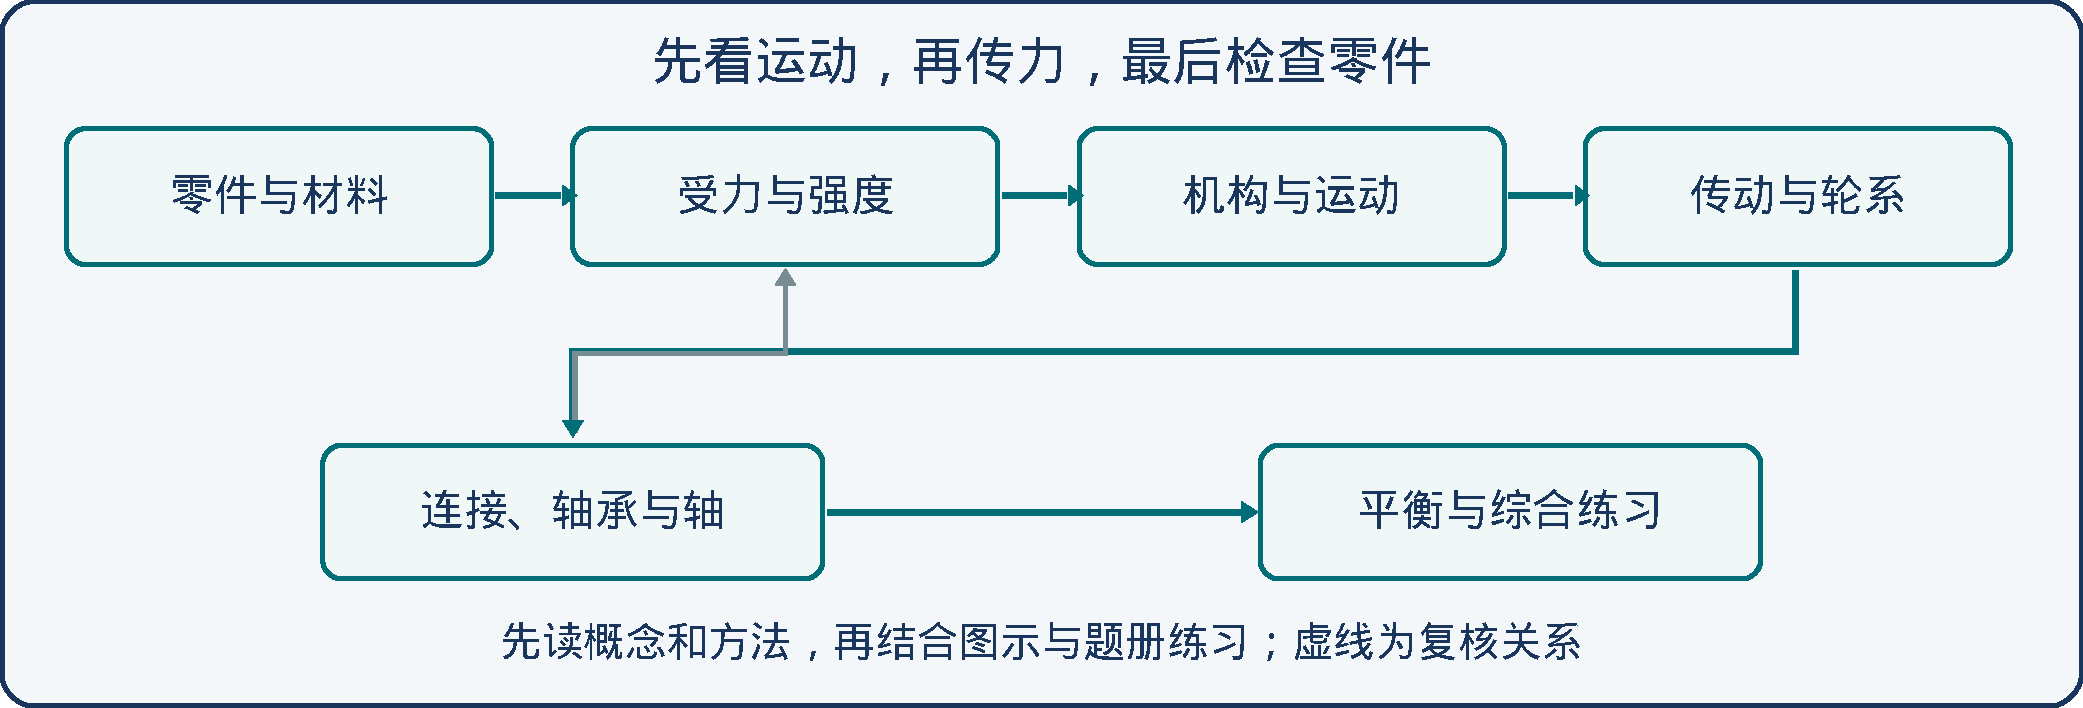
\includegraphics[width=.8\linewidth,height=8cm,keepaspectratio]{course-map-vector.pdf}\end{center}


图 0-1 全书知识地图（自绘）：沿实线建立知识顺序，再用受力和强度检查零部件。





\subsection{C-3407｜用户指定范围与待核对事项}
\label{c-3407}

用户还提出轴的力矩图、螺旋传动力和效率、四杆行程与 K、齿轮尺寸和受力、轮系计算、轴承寿命与设计验算、连接的预紧和查表，以及“不考间隙”。讲义已给出部分方法、公式、自编例题及原参考解答，但图题、部分公式条件和表格仍须回到原件核对，并非所有项目都只有范围记录或已完整验收；“必考”“不考”均为用户提供的复习信息，未独立验证。





\subsection{C-3408｜公式与例题补充（初步识别，待图文复核）}
\label{c-3408}

既有公式与例题补充依据资料 1 第 1—16 页和资料 2 第 6—8、13—14 页的离线 OCR 整理，现按主题分布于下文；OCR 对数学符号识别有限，题图与表格尚待复核。资料 2 为 2019—2020 学年第 1 学期试卷及其配套参考答案，不能据此推断本学期的考试范围。





\subsection{C-3416｜补充解题方法与自检}
\label{c-3416}

原补充方法与自检按主题归入下文：凸轮见 \hyperref[k-3418]{K-3418}，轮系见 \hyperref[k-3419]{K-3419}，轴的弯扭分析见 \hyperref[k-3417]{K-3417}，材料与平衡见 \hyperref[k-3420]{K-3420}、\hyperref[k-3421]{K-3421}。





\subsection{C-3423｜扩展知识与原件审校}
\label{c-3423}

原扩展知识按主题归入下文：凸轮见 \hyperref[k-3424]{K-3424}，齿轮见 \hyperref[k-3425]{K-3425}，带传动见 \hyperref[k-3426]{K-3426}，连接与轴承见 \hyperref[k-3427]{K-3427}、\hyperref[k-3428]{K-3428}。原件冲突和待核对事项保留在对应条目。





\subsection{C-3435｜图解与计算训练}
\label{c-3435}

标明自编的图形为按运动关系和受力条件\textbf{自编绘制}的教学示意，不是对原题图的逐像素描摹。粗实线和箭头分别表示构件与力的方向；坐标、力值及尺寸仅适用于本节示例。每个例题都先找几何或受力条件，再计算并检查结论。





\subsection{C-3405｜凸轮、齿轮与轮系}
\label{c-3405}

凸轮题需要区分基圆、理论轮廓与实际轮廓，并按从动件类型及反转法作图；压力角定义及滚子半径修正须结合具体机构。齿轮部分重点复习模数和齿数与尺寸的关系、配对条件、失效与强度校核，以及啮合力方向；外啮合平行轴斜齿轮配对时旋向相反。蜗杆传动受力应分别标出圆周力、径向力和轴向力，方向结合旋向、转向逐一判断。


轮系计算先区分定轴与周转部分，明确各轮和行星架的转速符号；周转轮系可采用转化机构法，在各构件角速度中减去行星架角速度后计算相对传动比。最终核对方向和输入输出构件。





\subsection{C-3406｜带、连接、轴承和轴}
\label{c-3406}

带传动复习类型、张紧和 V 带结构作图；连接复习螺栓、螺钉、双头螺柱适用情形以及预紧和强度校核。螺纹强度计算应使用与公式相符的危险截面直径，不能将大径、小径或题目给出的计算直径混同。


轴承复习代号、受力、当量动载荷和寿命。成对角接触球轴承或圆锥滚子轴承应先判断内部轴向力方向、压紧及放松，再求各轴承轴向载荷和各自当量动载荷；具体公式及系数以题目给定表格为准。轴的结构改错需检查轴向定位、装拆、配合、圆角与倒角是否干涉等。


联轴器通常在机器停止时拆装以分离两轴；离合器可在机器运转过程中按其结构实现接合或分离。静平衡要求质心位于转轴上，动平衡还要求合成不平衡力偶为零；动平衡满足静平衡，静平衡未必满足动平衡。


\section{一、零件、构件}

\begin{center}
\includegraphics[width=.8\linewidth,height=8cm,keepaspectratio]{chapter-map-01.pdf}\end{center}


图 1-1 零件、构件知识地图（自绘）。


\subsection{绪论｜自动化专业为什么学机械设计}

来源为用户于 2026-11-23 提供的课堂概要。课程学习常用机构和零部件的工作原理、设计方法及应用。以自动送料台为例（整理举例），控制器发出移动指令，电机提供转动，丝杠把转动变为直线运动，滑台把工件送到指定位置。即使控制指令准确，传动误差也会影响工件的实际位置。


\textbf{从整机看到零件。} 机械是机器与机构的总称。机器通过机械运动做功、转换能量或处理信息，可减轻人的劳动。机构关注运动和力怎样传递，由相互连接的构件组成。构件是运动单元，可以由一个或多个零件构成。零件是制造单元。按功能看，一台机器可分为驱动、传动和执行三部分。在送料台中，三者分别对应电机、丝杠传动和滑台。


\textbf{设计要回答四个问题。} 功能性看速度、精度、功率能否达到指标。可靠性看设备在规定条件和预期寿命内完成任务的能力。经济性要权衡性能与成本。社会性要考虑设备使用对人和环境的影响。


\textbf{从需求到投产。} 计划阶段确定需求并论证可行性。方案设计阶段比较不同实现方式并选定方案。技术设计阶段确定结构、材料和尺寸。试制实验阶段制作样机、测量性能并核对指标。投产后根据制造和使用反馈改进产品。


\textbf{发展与学习要求。} 课堂按古代人力机械、工业革命、现代计算机辅助设计回顾机械发展，并引出常用材料和结构工艺性。材料会影响零件能承受的载荷，也会影响加工方法。课程考核包括平时成绩和考试成绩，概要未给出具体比例或挂科率数值。课堂建议及时复习、完成作业，有疑问时及时提问。


\textbf{自检（整理举例）。} 两块钢板分别加工后焊成一个刚性支架，在机构简图中一共算几个构件？答：两个制造零件固连后没有相对运动，按一个构件处理。





\subsection{C-3401｜基本概念与强度}
\label{c-3401}

零件是制造的基本单元，构件是运动的基本单元；一个构件可以由多个零件组成。 例如，B091-01 第 6 页将连杆体、连杆盖、螺栓、螺母、垫圈、套筒和轴瓦作为连杆装配图中的零件示例；分析时按实际相对运动判断哪些零件合成一个构件。常见基本变形有拉伸、压缩、弯曲、扭转和剪切。强度校核应将危险截面的计算应力与对应许用应力比较，载荷性质与应力类型不同，许用值不能混用。


正火与退火是不同的加热、保温及冷却工艺；淬火后高温回火称调质。Q235 的 Q 表示屈服强度，数字表示规定条件下的屈服强度数值，单位通常为 MPa，并非含碳量。优质碳素结构钢 45 的数字表示平均含碳量约 0.45\%；不同牌号体系不能套用同一解释。





\subsection{K-3420｜材料怎么选，钢为什么要热处理}
\label{k-3420}

来源为用户提供的材料课章节概要（00:00、11:01、20:12、31:14）及资料 1 第 1 页。下文的典型分界值、零件例子和自检为整理补充。


\textbf{00:00｜从零件的工作环境认识三类材料。} 金属材料包括钢、铸铁等铁基材料，以及铜、铝等非铁金属及其合金。非金属材料包括工程塑料、橡胶和玻璃。例如，密封圈要能压缩并回弹，可选橡胶。复合材料把作用不同的材料结合起来，例如碳纤维增强树脂和玻璃纤维增强树脂，纤维承载，树脂把纤维连成整体并传递载荷。航空和交通结构看重的是在满足强度要求的同时减轻重量。


\textbf{11:01｜先看按什么分类，再读牌号。} 钢和铸铁都是铁碳合金。基础课程在铁碳相图上常以约 2.11\% 碳为界。铸钢是浇铸成形的钢，铸铁同样可以浇铸，“铸”字说明成形方法，不能单凭这个字判断材料。钢按用途可分为结构钢、工具钢和特殊性能钢。按碳的质量分数，碳钢常分为低碳钢（不超过约 0.25\%）、中碳钢（约 0.25\% 至 0.60\%）和高碳钢（高于约 0.60\%）。具体分界按课程教材。一般在组织状态可比时，含碳量增加，硬度提高，塑性和焊接性下降。低碳钢适合焊接支架，中碳钢经适当热处理可制轴，高碳钢可用于需要硬度的工具。


Q235 中的 235 表示规定条件下的屈服强度数值，单位为 MPa。45 钢中的 45 表示平均含碳量约 0.45\%，据此可判断为中碳钢。合金结构钢还通过锰、铬等元素调节淬透性等性能。需要导电可考虑铜，需要减重可考虑铝合金，轻载且要求绝缘时可考虑工程塑料。


\textbf{20:12｜用加热、保温和冷却改变钢的内部组织。} 同一钢种采用不同热处理，可以得到不同的硬度、韧性和加工性能。课堂所说的“四火一调质”包括下列工艺。冷却快慢要结合钢种和截面判断。


\begin{longtable}{p{4.86cm}p{4.86cm}p{4.86cm}}
\toprule
工艺 & 怎样处理 & 选它解决什么问题 \\

\midrule
\endhead
退火 & 加热保温后缓慢冷却，常随炉冷却 & 软化材料、改善切削加工性，或按工艺消除内应力 \\
正火 & 加热至适宜温度后保温，在空气中冷却 & 细化组织，为后续加工或热处理作准备 \\
淬火 & 加热使组织奥氏体化，再以足够速度冷却 & 可获得以马氏体为主的高硬度组织，同时会带来内应力和脆性 \\
回火 & 淬火后再次加热到低于临界点的适宜温度，保温后冷却 & 降低淬火应力，按用途调整硬度与韧性 \\
调质 & 淬火后接高温回火 & 获得较好的强度和韧性配合，常用于受力的轴类件 \\
\bottomrule
\end{longtable}

\textbf{31:14｜按工作部位决定工艺。} 低温回火着重保留硬度和耐磨性，中温回火常用于弹簧以获得较高弹性极限，高温回火常与淬火配合用于受力结构件。若只要求表层耐磨、心部仍要承受冲击，可考虑化学热处理。渗碳使表层富碳，通常再淬火、低温回火。渗氮使表层富氮，可提高表面硬度。碳氮共渗同时向表层引入碳和氮。


\textbf{选材自检（自编）。} 一根反复承受弯矩和扭矩的传动轴，为什么可以先考虑 45 钢调质？先看使用要求，轴既要承载又要有韧性。再看工艺要求，要能加工成形，且轴径应与材料的淬透性匹配。最后看经济性，把材料、加工和热处理费用一起比较。若轴径较大，45 钢难以获得所需心部性能，就要重新比较合金结构钢方案。





\subsection{K-3508｜结构工艺性、标准化与零件失效}
\label{k-3508}

来源为用户提供的课堂概要。四个时间点对应本节四段。扳手空间和磨损现象的自检为整理补充。


\textbf{01:21｜从毛坯到装配看零件形状。} 毛坯是还要继续加工的零件雏形。在满足使用要求的前提下，设计时依次问三个问题：毛坯能否方便地做出来？刀具能否伸到加工面？装配时能否准确定位，检修时能否拆下？铸件沿起模方向留斜度，模型就容易从砂型中取出。模锻件选简单平整的分模面，便于制模和取件。冲压件在功能允许时采用对称形状，有助于板料均匀变形。三种设计都从各自的制造步骤出发。


\textbf{13:50｜检查工具能不能用，再考虑规格能不能共用。} 例如箱体上的螺栓孔即使钻得出来，旁边的筋板也可能挡住套筒或扭矩扳手。画装配图时，要同时检查螺栓插入方向、套筒外径、扳手摆动和拆出空间。结构工艺性的三项要求可用历年卷第 11 题自测。


标准化把经常重复的要求统一起来。把同类产品按尺寸或能力排成一组规格，称为系列化。让多种产品共用同一规格的零部件，称为通用化。统一产品质量要求和检验方法，有助于批量生产时按同一条件验收。采用通用紧固件，设计时可以直接选型，生产时减少换装，维修时也容易找到备件。


\textbf{26:56｜读国标代号，再按载荷判断工作能力。} 强制性国家标准代号为 GB，推荐性国家标准代号为 GB/T。概要中的“GDP”据《国家标准管理办法》第三十二条校正。课堂在此提醒复习“四火一调质”，五种工艺见 K-3420。检查工作能力时先判断载荷随时间怎样变化：持续不变的载荷、反复变化的载荷和突然施加的冲击载荷，会使同一零件面对不同的失效风险。一次过载可能引起整体断裂。循环应力可能使细小裂纹从轴肩、键槽等应力集中处萌生并逐步扩展，最后发生疲劳断裂。应力幅、循环次数、缺口和表面状态都会影响疲劳寿命。


\textbf{39:53｜用现象辨认五项失效。} 失效指零件已无法满足预定功能。课堂列出的前三项是表面损伤，后两项可在零件仍完整时影响运行精度。


\begin{longtable}{p{7.51cm}p{7.51cm}}
\toprule
现象 & 形成原因与辨认线索 \\

\midrule
\endhead
磨损 & 接触面相对运动使材料逐渐损失。例如轴颈逐渐变细，配合间隙随使用时间增大。 \\
胶合 & 润滑膜破坏后，两表面的微小接触区黏着，再被相对滑动撕开，常留下沿滑动方向的拉伤。高速重载产生的局部高温易引起热胶合，低速重载也可能因油膜难以建立而发生冷胶合。概要中的“交合”按机械术语校为“胶合”。 \\
点蚀 & 齿面等部位反复承受接触应力，表层材料因疲劳而小片剥落，留下小坑。 \\
变形过大 & 轴受力时即使只发生可恢复的弹性挠曲，也可能使齿轮啮合偏斜。卸载后仍留下的永久变形属于塑性变形。 \\
振动过大 & 周期性激励等原因使零件往复摆动。振幅超过允许范围时，加工或定位精度会下降。 \\
\bottomrule
\end{longtable}

\textbf{自检。} \textcircled{1} 螺栓可以穿过安装孔，但扭矩扳手转不开，应该改哪里？答：调整孔或筋板的位置，给工具留出操作空间。\textcircled{2} 齿面出现成片小坑，应优先检查什么？答：接触疲劳和点蚀。若看到的是沿滑动方向的撕伤，则应进一步检查润滑和胶合。


\textbf{作业讲评 07:35—11:01｜三个填空放在一起记。} 零件按制造数，构件按相对运动数，焊死的几块板可以是一个构件。正火通常加热保温后空冷，调质是淬火后高温回火。45 钢的 45 表示平均碳质量分数约 0.45\%；Q195 中的 195 表示屈服强度等级，单位 MPa。


\needspace{12\baselineskip}


\subsection{本章复盘}

\begin{longtable}{p{7.51cm}p{7.51cm}}
\toprule
问题 & 三句话带走 \\

\midrule
\endhead
是什么 & 零件是制造单元，构件是运动单元。 \\
为什么 & 同一构件可以由多个没有相对运动的零件组成。 \\
边界 & 按运动数构件时，不按零件数量直接相加。 \\
\bottomrule
\end{longtable}

\section{二、应力、受力分析：拉、压、弯、扭、剪}

\begin{center}
\includegraphics[width=.8\linewidth,height=8cm,keepaspectratio]{chapter-map-02.pdf}\end{center}


图 2-1 应力、受力分析：拉、压、弯、扭、剪知识地图（自绘）。


基础强度及五种变形的概述见 \hyperref[c-3401]{C-3401}。





\subsection{K-3509｜从拉伸曲线读出材料性能，再校核零件}
\label{k-3509}

来源为用户提供的课堂概要。下图按典型低碳钢工程应力应变曲线绘制，仅表示趋势。例题数据为自编。


\textbf{00:00｜先问零件怎样失去工作能力。} 轴可能整体断裂，齿面可能点蚀，细长杆可能挠曲到无法准确定位。磨损、振动等因素也可能共同造成综合失效。强度衡量零件抵抗断裂或过量塑性变形的能力。刚度衡量它抵抗弹性变形的能力。例如机床主轴卸载后能恢复原状，但切削时挠度过大仍会影响加工精度，因此还要单独校核刚度。选设计准则时，要结合载荷、允许变形、转速、温度和预期寿命，必要时检查振动稳定性、耐热性和可靠性。


\textbf{13:46｜看载荷怎样作用，再判断变形。} 沿杆轴线拉或压，主要改变杆长。两侧的横向力使相邻截面有错开的趋势，形成剪切。销钉与孔壁相互压紧，还会在接触面产生局部挤压，同一个销连接可能要分别验算剪切和挤压。绕杆轴线的力偶使截面相对转动，形成扭转。横向载荷使杆轴线变弯，形成弯曲。课堂将拉伸与压缩合讲、剪切与挤压合讲，再讲扭转和弯曲，共四组。


\textbf{26:12｜沿低碳钢曲线从左向右读。} 拉伸试验逐步增加拉伸变形，记录拉力和标距变化。纵轴为工程应力 $\sigma=F/A_0$，横轴为工程应变 $\varepsilon=(L-L_0)/L_0$。其中 $A_0$ 和 $L_0$ 均取试验前的数值。


\begin{center}
\begin{tikzpicture}[x=1cm,y=.72cm,>=stealth]
\draw[->] (0,0)--(10,0) node[right] {$\varepsilon$};
\draw[->] (0,0)--(0,4.5) node[above] {$\sigma$};
\draw[very thick,navy] (0,0)--(1.35,2.6)--(1.5,2.35)--(2.7,2.38) .. controls (4.1,3.4) and (5.4,3.8) .. (6,3.8) .. controls (7,3.78) and (8.2,3.1) .. (8.8,2.8);
\fill (6,3.8) circle (2pt) node[above] {抗拉强度};
\fill (8.8,2.8) circle (2pt) node[right] {断裂};
\node at (.75,.45) {弹性};\node at (2.1,1.8) {屈服};\node at (4.3,2) {强化};\node at (7.4,2) {颈缩};
\end{tikzpicture}
\end{center}


弹性阶段卸载后可恢复，其中起始直线段满足 $\sigma=E\varepsilon$，斜率 $E$ 是弹性模量。进入屈服阶段后，应力变化很小，应变仍明显增长，卸载后会留下塑性变形。概要将屈服极限标在原课件的 c 点，做题时按题图识别上下屈服点。强化阶段要继续提高应力才能使试样进一步均匀伸长。最高点对应抗拉强度 $R_m=F_{\max}/A_0$。随后变形集中在局部，截面迅速缩小，称为颈缩。此时拉力下降，所以用原始面积计算的工程应力也下降，直至断裂。


\textbf{38:54｜比较塑性，再选强度计算依据。} 把断开的试样对合，量断后标距 $L_u$ 和断口处最小截面积 $A_u$。断后伸长率为 $(L_u-L_0)/L_0\times100\%$，断面收缩率为 $(A_0-A_u)/A_0\times100\%$。前者反映标距内留下的伸长，后者反映断口附近的收缩。相同试验条件下，低碳钢拉断前通常能观察到明显的塑性伸长和颈缩。灰铸铁在拉伸时塑性变形小，通常没有明显的屈服平台。


\textbf{强度条件及三种问法（自编例题）。} 对承受静拉力的等截面杆，工作应力应满足 $F/A\leq[\sigma]$。许用应力等于相应极限应力除以安全系数。对延性材料按防止屈服设计时取屈服强度，对脆性材料做单向静拉断裂校核时常取抗拉强度。安全系数给材料和载荷的不确定性留出余量，实际题目按给定工况取值。


设拉杆屈服强度为 240 MPa，题给安全系数为 2，则许用应力为 120 MPa，即 120 N/mm$^{2}$。忽略应力集中，只考虑均匀静拉伸。


\begin{longtable}{p{4.86cm}p{4.86cm}p{4.86cm}}
\toprule
题目给什么 & 求什么 & 代入同一强度条件 \\

\midrule
\endhead
拉力 12 kN，面积 120 mm$^{2}$ & 校核强度 & 工作应力为 12000/120=100 MPa，小于 120 MPa，满足条件。 \\
拉力 12 kN & 设计最小面积 & 面积至少为 12000/120=100 mm$^{2}$。 \\
面积 120 mm$^{2}$ & 确定许可载荷 & 拉力至多为 120$\times$120=14400 N，即 14.4 kN。 \\
\bottomrule
\end{longtable}

\textbf{自检。} 同材料、同截面、同拉力下，把杆长加倍，强度和变形怎样变化？答：均匀拉应力仍为 $F/A$。在线弹性范围内，伸长量 $FL/(EA)$ 加倍。因此满足强度条件的杆仍可能超过允许伸长量。





\subsection{K-3510｜从截面突变到销连接，再到轴的扭矩图}
\label{k-3510}

依据本节课堂概要的四个时间点整理。概要提到电瓶车挂钩和多转子轴，未给原题尺寸及数值。下列图形、尺寸和载荷均为自编训练条件。


\textbf{01:09｜强度计算先选截面。} 轴向载荷 $F$ 作用在均匀直杆上，远离载荷作用处的平均正应力大小为 $|F|/A$。计算值应满足 $|F|/A\leq[\sigma]$。静拉伸时，塑性材料通常以屈服强度、脆性材料通常以抗拉强度为依据，再除以相应安全系数得到许用应力。脆性材料受压时应采用抗压数据。校核、求所需面积、求许可载荷的换算见 K-3509。


\textbf{12:32｜孔边为何容易起裂？} 拉板开孔后，孔所在截面的净面积减小。即使已用净面积计算平均应力，孔边各点承受的应力仍不均匀，局部峰值可能明显高于平均值。轴肩、槽底和尖角也会出现应力集中。在线弹性计算中可用 $K_t=\sigma_{\max}/\sigma_{\rm nom}$ 表示放大程度，名义应力的面积取法应与系数表一致。反复加载时，这些部位尤其容易萌生疲劳裂纹。轴肩改用圆角或平缓过渡，可减轻应力集中，同时要确认圆角不会顶住相邻零件。


看铆钉或销连接时，先想象两块板相对滑动。板的交界处像剪刀一样横向剪销，该处要检查销的横截面。销同时压住孔壁，局部接触区要检查挤压。前者的力沿剪切面，后者按接触压力合力方向取投影面积。直径为 $d$ 的圆销穿过厚度为 $t$ 的平板时，常用的名义挤压面积是 $dt$。


\textbf{23:32｜挂钩销连接：哪一处先达到许用应力？} 设一块中耳板夹在两块相同外耳板之间，用直径 10 mm 的销连接。中板受拉力 $F$，两外板对称均载，各承受 $F/2$。忽略摩擦、偏载和销的弯曲，只比较销剪切与孔壁挤压。中板厚 6 mm，每块外板厚 4 mm。给定销的许用切应力 60 MPa，各接触副的许用挤压应力 100 MPa。


\begin{center}
\begin{tikzpicture}[>=stealth]
\foreach \x/\w/\lab in {0/1/外板,1/1.5/中板,2.5/1/外板}{
\draw[fill=tealaccent!8] (\x,0) rectangle (\x+\w,1.4);
\node at (\x+\w/2,1.12) {\lab};}
\draw[fill=gray!30] (-.35,.45) rectangle (3.85,.68);
\foreach \x in {1,2.5}{\draw[dashed,navy,thick] (\x,.12)--(\x,.94);}
\draw[->,thick] (1.75,1.4)--(1.75,2) node[right] {$F$};
\foreach \x in {.5,3}{\draw[->,thick] (\x,0)--(\x,-.55) node[right] {$F/2$};}
\node[right] at (3.85,.56) {销};
\end{tikzpicture}
\end{center}


图中两条虚线标出剪切面。每面面积 $A=\pi d^2/4$，每面承受 $F/2$。由 $F/(2A)\leq[\tau]$ 得销的剪切许可拉力约为 9.42 kN。中板孔壁传递完整的 $F$，由 $F/(10\times6)\leq100$ 得 $F\leq6.00$ kN。每块外板由 $(F/2)/(10\times4)\leq100$ 得 $F\leq8.00$ kN。于是三项同时满足时许可拉力为 \textbf{6.00 kN，由中板挤压控制}。自检：代入 6000 N，销的平均切应力约 38.2 MPa，中板和外板的挤压应力分别为 100 MPa 和 75 MPa。


\textbf{36:24｜先定观察方向，再画扭矩图。} 若双手在方向盘两侧施加大小相等、方向相反的切向力，每个力为 $Q$，两作用线间距为 $D$，则力偶矩大小为 $QD$。轴受扭后，相邻截面绕轴线发生相对转动。令轴线从左往右为正，右手拇指指向右方时，四指弯曲方向就是正转向。从右端向左看为逆时针。功率与外加转矩满足 $P=M\omega$。取功率大小为 kW、转速大小 $n$ 为 r/min，则 $|M|=9550P/n$，单位 N·m。数值公式给出大小，输出负载对轴的反扭矩方向与轴的转向相反。


自编例：从左到右依次是转子 A、B、C。轴以 955 r/min 沿正向匀速转动，A 输入 6 kW，B、C 分别取走 2 kW、4 kW，忽略损失。三处施加于轴的外力矩依次为 +60、$-$20、$-$40 N·m，代数和为零。切开轴并保留右段，约定左段作用于右段的正向力矩为正。AB 段右侧负载合计 $-$60 N·m，故截面内扭矩为 +60 N·m。BC 段只剩 C 的负载，内扭矩为 +40 N·m。由左至右画扭矩图，在 A 处从 0 跳至 60，在 B 处降至 40，在 C 处回到 0，两转子间画水平线。单段图形可对照 K-3438。





\subsection{K-3511｜从电机功率画扭矩图，从梁的载荷画弯矩图}
\label{k-3511}

依据用户提供的四段课堂概要。轴例沿用 K-3510 的自编数据，梁例与图为自编。


\textbf{01:18｜转矩公式里的数字从哪里来？} 电机轴每转一圈转过 $2\pi$ 弧度。转速为 $n$ r/min 时，角速度为 $\omega=2\pi n/60$ rad/s。设轴端机械输出功率为 $P$ kW，则 $1000P=T\omega$，转矩大小为


\[T=\frac{60000}{2\pi}\frac{P}{n}\approx9550\frac{P}{n}\quad(\mathrm{N\cdot m}).\]


概要中的“950”和“p=9550”按上述推导校正。若功率用 W，系数约为 9.55。例：6 kW、955 r/min 对应约 60 N·m。数值算出大小后，再判断方向。右手四指沿转动方向弯曲，拇指给出角速度方向。输入动力矩沿转向，取走功率的负载对轴施加反向力矩。


\textbf{13:41｜由扭矩图找危险截面。} 匀速且忽略损失时，整轴外力矩代数和为零。沿上节轴线从 A 向 C 走，依次遇到 +60、$-$20、$-$40 N·m。按上节截面约定，图线依次跳至 +60、+40、0。集中力矩处发生跳变，两转子之间没有分布力矩，图线保持水平。


对线弹性圆轴作纯扭转分析，横截面上只有切应力，大小随半径线性增加，外缘最大。强度条件为 $\tau_{\max}=|T|/W_p\leq[\tau]$，其中 $W_p$ 是抗扭截面系数。等直径实心圆轴有 $W_p=\pi d^3/16$。设上例轴径为 20 mm，许用切应力为 50 MPa。AB 段有全轴最大的扭矩大小，取 60000 N·mm，得最大切应力约 38.2 MPa，满足该纯扭转校核。若轴径分段变化，应逐段比较 $|T|/W_p$，细轴段也可能控制强度。


\textbf{24:25｜把梁切开，剪力和弯矩从哪里来？} 横向力或横向平面内的外力偶能使梁的轴线弯曲。截开梁并取其中一段，另一段的作用可以用截面内力表示。在下面的平面问题中，竖直方向的力平衡求剪力 $V$，对切口取矩求弯矩 $M$。先算支反力，再按载荷位置分段。


\textbf{33:05｜固定符号约定，再列方程。} 概要中的“弯距”统一写作“弯矩”。取梁下缘受拉、弯成微笑形为正弯矩，上缘受拉为负弯矩。保留切口左段时，约定切口上向下的剪力为正、逆时针的弯矩为正。取右段时，对应箭头反向，算得的截面内力符号应一致。


自编梁例：A、B 简支，跨度 2 m，跨中 C 受向下集中力 800 N。两支反力各向上 400 N。以 A 为原点，$x$ 用 m。对 AC 段切口取左段，竖直平衡给出 $400-V=0$，对切口取矩有 $M-400x=0$。当切口越过 C，还要把 800 N 及其力臂 $x-1$ 纳入平衡。结果如下。


\begin{longtable}{p{4.86cm}p{4.86cm}p{4.86cm}}
\toprule
切口位置 & 剪力 V（N） & 弯矩 M（N·m） \\

\midrule
\endhead
A 与 C 之间 & +400 & $400x$ \\
C 与 B 之间 & $-$400 & $400x-800(x-1)=800-400x$ \\
\bottomrule
\end{longtable}

\begin{center}
\begin{tikzpicture}[x=1.15cm,y=.65cm,>=stealth]
\draw[->] (0,0)--(4.4,0);\draw[thick,navy] (0,0)--(2,1.8)--(4,0);
\node[above] at (2,1.8) {$+400\,\mathrm{N\cdot m}$};
\foreach \x/\l in {0/A,2/C,4/B}{\node[below] at (\x,0){\l};}
\node at (2,-1) {弯矩图（正值画在上方）};
\draw[->] (5,0)--(9.4,0);\draw[thick,tealaccent] (5,1)--(7,1)--(7,-1)--(9,-1);
\node[above] at (6,1) {$+400\,\mathrm N$};\node[below] at (8,-1) {$-400\,\mathrm N$};
\node at (7,-2.2) {剪力图};
\end{tikzpicture}
\end{center}


\textbf{检查与辨析。} 两端弯矩均为零，跨中从左右两式算得同一个 +400 N·m。集中力使剪力跳变，使弯矩图的斜率改变。对细长梁估算挠度时常可忽略剪切变形，列力平衡时仍要保留剪力。若换成左端固定、右端向下受力的悬臂梁，固定端附近上缘受拉，按同一规定弯矩为负。





\subsection{K-3512｜从一次弯曲强度校核到反复受力的疲劳寿命}
\label{k-3512}

来源为用户提供的四段课堂概要。梁的尺寸、循环应力数值和寿命练习均为整理举例。概要中“弯距”统一为“弯矩”。根据 28:45 后文关于恒定外力和运动零件的描述，将“净载荷”“循环盈利”分别按“静载荷”“循环应力”理解。


\textbf{01:05｜用弯矩找最危险的材料点。} 沿用 K-3511 的简支梁，跨度 2 m，跨中 C 受向下的 800 N 力。对 A 取矩，得 B 处反力为 400 N，再由竖直力平衡得 A 处反力也是 400 N。在距 A 为 $x$ 的位置切开并取左段，AC 段有 $M=400x$，CB 段有 $M=400x-800(x-1)$（$x$ 用 m，$M$ 用 N·m）。两段在 C 处都给出 +400 N·m。按下缘受拉为正的约定，跨中下缘受拉，上缘受压，过了 C 后弯矩逐渐减小至零。


对同质、线弹性、上下对称截面的梁，弯曲正应力条件为 $|M|/W\leq[\sigma]$。抗弯截面系数 $W=I/y_{\max}$，其中 $I$ 为对中性轴的截面二次矩，$y_{\max}$ 为最外缘到中性轴的距离。自编截面取宽 20 mm、竖向高度 40 mm 的实心矩形，则 $W=bh^2/6\approx5333$ mm$^{3}$。跨中最大弯曲正应力约为 $400000/5333=75$ MPa。这个计算给出某一载荷下的峰值。评估疲劳还要知道同一点的应力如何随时间变化。


\textbf{17:38｜先分清比较对象，再算循环参数。} 名义载荷由给定功率、转速或外力等求得。若题目给定载荷系数 $K$ 来计入工况影响，则计算载荷为名义载荷的 $K$ 倍，再由它计算相应的正应力或切应力。静载荷的大小和方向对所选参考系保持不变。变载荷随时间变化。变应力可呈随机变化，也可按确定规律变化。若各循环重复同样的最大、最小应力，可用以下参数描述稳定循环。


\[\sigma_m=(\sigma_{\max}+\sigma_{\min})/2,\qquad \sigma_a=(\sigma_{\max}-\sigma_{\min})/2,\qquad r=\sigma_{\min}/\sigma_{\max}.\]


前两式分别是平均应力和应力幅，应力比的分母须非零。拉应力取正，压应力取负。由 +80 到 $-$80 MPa 时，平均值为 0，应力幅为 80 MPa，$r=-1$，属于对称循环。由 0 到 +80 MPa 时，平均值与应力幅均为 40 MPa，$r=0$，属于脉动拉伸。恒为 +80 MPa 时，应力幅为 0，$r=1$，对应静应力。


\textbf{28:45｜在旋转轴表面标一个点。} 水平圆轴承受方向固定的横向力，在空间中形成方向固定的弯矩。标记点随轴转到截面下缘时受拉，半圈后转到上缘受压，再转半圈回到原处。若只有该恒定弯矩，且没有附加轴向应力，表面点每转一圈经历一次对称弯曲循环。运动方式和受力方向一起决定应力是否交替。


疲劳破坏经历裂纹萌生、裂纹逐步扩展、剩余截面瞬时断裂三个阶段。轴肩圆角、加工划痕处的局部应力较大，可能先出现微裂纹。反复加载使裂纹增长，直到剩余截面无法承载。高周疲劳可发生在名义最大应力低于屈服强度时，即使材料有较好的塑性，整体也可能看不到明显的永久变形。设计时可改善圆角和表面质量、降低交变载荷，使用中可在应力集中部位安排适合材料及缺陷位置的无损检测。


\textbf{39:14｜用疲劳曲线回答“能承受多少次”。} 在指定材料状态、应力比和试验条件下，让多组试样分别承受不同应力幅，记录各试样失效时的循环次数 $N$。把结果作图并拟合，即得 S–N 曲线。下图为定性示意，横轴为循环次数的对数，纵轴为应力幅。图中平台只表示具有明显疲劳极限的一类材料和试验条件。


\begin{center}
\begin{tikzpicture}[x=1.05cm,y=.7cm,>=stealth]
\draw[->] (0,0)--(7,0) node[right] {$\log N$};
\draw[->] (0,0)--(0,3.6) node[above] {$\sigma_a$};
\draw[thick,navy] (.6,3.1)--(4.6,1.05)--(6.7,1.05);
\draw[dashed,tealaccent] (0,2.08)--(2.6,2.08)--(2.6,0);
\node[above right] at (4.6,1.05) {平台示意};
\node[below] at (2.6,0) {对应寿命};
\end{tikzpicture}
\end{center}


已知应力幅，水平找到曲线，再向下读疲劳寿命。已知目标寿命，则反向读取该寿命对应的疲劳强度。低周疲劳中循环塑性变形明显，常采用应变与寿命的关系描述。有明显平台时，在相应条件下可把长寿命区的极限应力幅作为疲劳极限。没有明显平台的材料通常报告指定循环数下的疲劳强度。实际零件使用试样数据时，还需考虑尺寸、表面状态、缺口和可靠度。


\textbf{自检（自编有限寿命算例）。} 假设题给某材料在相同应力比下的拟合关系为 $N\sigma_a^m=C$，斜段内 $m=3$，应力幅 120 MPa 时寿命为 100 万次。取 150 MPa，且仍在该斜段内，则寿命约为 $10^6(120/150)^3=512000$ 次。若转速为 1000 r/min 且每转一个循环，对应约 8.53 小时。指数和基准点均为练习设定，不能直接套用到其他材料。





\subsection{K-3422｜资料 1 第 1—4 页的补充与审校}
\label{k-3422}

\begin{itemize}
\item 
材料牌号：原件列 Q195、Q235，ZG230—450 和 HT200。原件用 20Mn2 示例说明平均含碳量 0.20\%、锰含量约 2\%；不同牌号按对应标准和版本解释。


\item 
应力循环特性 r=$\sigma$min/$\sigma$max（$\sigma$max 非零）：原件列 r=$-$1 为对称循环、r=0 为脉动循环、0<|r|<1 为其列举的非对称循环，r=1 为静应力。具体应力符号与循环边界依题意。


\item 
普通螺旋副位移 l=P$_{h}$$\varphi$/(2$\pi$)。资料 1 第 3 页差动螺旋机构按该图的符号约定给 l$_{2}$=(P$_{h}$A$-$P$_{h}$B)$\varphi$$_{1}$/(2$\pi$)，右旋导程取正、左旋取负；方向必须与原图的观察方向和转角约定一致。


\item 
\textbf{原文差异}：资料 1 第 3 页将自锁边界写作升角$\le$摩擦角或当量摩擦角，而用户考点与试卷答案写“小于”。等号为理想极限平衡，实际判断建议采用严格小于；考试以教师定义为准。


\item 
\textbf{待核对}：资料 1 第 1 页把中径写为大径与小径的算术平均值。中径应按牙型上牙厚与牙槽宽相等的位置定义，不能无条件把这个平均关系用于所有标准螺纹。



\end{itemize}




\subsection{K-3417｜轴的载荷和弯扭组合（整理说明）}
\label{k-3417}

轴上外力应先化到轴的作用位置，再在两个互相垂直的平面分别建立受力图。先分别根据力与力矩平衡求支承反力，画两个平面的弯矩图 M$_{1}$(x)、M$_{2}$(x)，同一截面的合成弯矩 M(x) 为 (M$_{1}$$^{2}$+M$_{2}$$^{2}$) 的平方根；由各传动件施加的扭矩画扭矩图 T(x)。平面名称取决于题目给的坐标：扭矩是绕轴线的力矩，不能把某个坐标平面固定称为“扭矩面”。在阶梯、键槽、载荷作用处等危险截面做弯扭强度校核，并按题目要求考虑应力循环和应力集中。没有具体图、尺寸和载荷，不能算出反力或危险截面数值。


自检：两个垂直平面内某截面弯矩分别为 3 N·m 和 4 N·m，合成弯矩为多少？答：5 N·m；不可将弯矩代数直接相加。





\subsection{K-3438｜轴的支反力、两平面弯矩和扭矩图}
\label{k-3438}

【来源】用户提出的轴受力与力矩图要求；以下为自编、静定、忽略轴重的例题。轴 A、B 两支承相距 2 m，C 为中点；C 处有垂直向下载荷 800 N 和水平载荷 600 N。C 处由电机输入 200 N·m，B 端由工作机输出大小相同的扭矩。求两个正交平面的支反力、弯矩、扭矩及 C 截面合成弯矩。


\begin{center}
\begin{tikzpicture}[x=1.15cm,y=.9cm,>=stealth]
\draw[very thick] (0,3)--(4,3); \foreach \x/\l in {0/A,4/B} {\fill (\x,3) circle (1.8pt);\node[above] at (\x,3.1) {\l};} \fill (2,3) circle (1.8pt); \node[below] at (2,2.95) {C};
\draw[->,thick,navy] (2,4.15)--(2,3.08) node[midway,right] {800 N};
\draw[->,thick,tealaccent] (0,2)--(0,2.92) node[midway,left] {400 N};
\draw[->,thick,tealaccent] (4,2)--(4,2.92) node[midway,right] {400 N};
\node at (2,1.6) {垂直平面受力；$AC=CB=1\,\mathrm{m}$};
\draw[->] (5.6,2.5)--(10.1,2.5); \draw[thick,navy] (5.8,2.5)--(7.8,3.55)--(9.8,2.5);
\node at (7.8,3.84) {$400\,\mathrm{N\!\cdot m}$}; \node[right] at (10,3.0) {垂直面弯矩图};
\draw[->] (5.6,.6)--(10.1,.6); \draw[thick,tealaccent] (5.8,.6)--(7.8,1.35)--(9.8,.6);
\node at (7.8,1.58) {$300\,\mathrm{N\!\cdot m}$}; \node at (7.8,.15) {水平面弯矩图};
\end{tikzpicture}
\end{center}


【解】由两平面分别列平衡方程：垂直面支反力均为 400 N，水平面支反力均为 300 N，方向各自与对应载荷相反。两弯矩图均为三角形，C 截面大小分别是 400 N·m、300 N·m，合成弯矩为 500 N·m。轴向位置 0<x<1 m 的 A—C 段扭矩为 0，1<x<2 m 的 C—B 段扭矩大小为 200 N·m；示例截面图采用大小表示，正负号须依题设坐标和截面约定。C 处存在外加集中扭矩，画扭矩图时在 C 发生跳变。图未示水平面力箭头，其受力图与垂直面相同，只需把 800、400 分别换成 600、300 N。


以下是按本例力矩符号约定绘制的扭矩大小图；C 点外加扭矩使曲线从 0 跳至 200 N·m，B 点外力矩使其回到 0。


\begin{center}
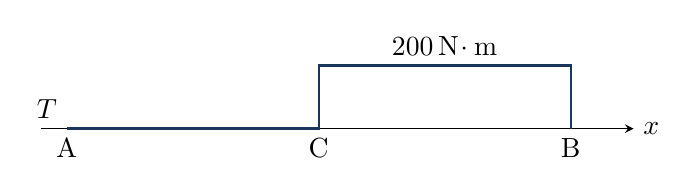
\begin{tikzpicture}[x=1.6cm,y=.8cm,>=stealth]
\draw[->] (-.2,0)--(4.5,0) node[right] {$x$};
\draw[thick,navy] (0,0)--(2,0)--(2,1)--(4,1)--(4,0);
\foreach \x/\label in {0/A,2/C,4/B} {\node[below] at (\x,0) {\label};}
\node[above] at (3,1) {$200\,\mathrm{N\!\cdot m}$};
\node[above left] at (0,0) {$T$};
\end{tikzpicture}
\end{center}


【检查】每个平面分别满足合力和合力矩为零；弯矩合成是在同一截面上作矢量合成；强度验算还需截面直径、危险截面及材料许用值，本题未提供，不能直接给出安全结论。


\textbf{作业讲评 11:37—13:50｜2-13：先指认破坏面。} 环形端面承压，有效面积为 $\pi$(D$^{2}$$-$d$^{2}$)/4；若沿直径 d$_{s}$ 的圆柱面剪断，有效剪切面积为 $\pi$d$_{s}$h，h 是剪切面的轴向高度。两次分别用对应载荷除以面积，与各自许用应力比较。求允许载荷时取两项限值中较小者。


\textbf{14:34—30:27｜画扭矩图和 2-17 弯矩图。} 横坐标沿轴或梁的长度，纵坐标注明 T 或 M 和正方向。自由轴先核对外力矩平衡；固定端若有未知反扭矩，先由整体平衡求出。沿集中力矩逐段截开，段内无分布扭矩时 T 为常量。画梁的弯矩图先用整体力矩平衡求支反力，再按载荷位置分段；截面左右选未知量较少的一侧。集中力偶使弯矩图跳变，集中力使剪力跳变。抄图前先用截面平衡验符号。


\needspace{12\baselineskip}


\subsection{本章复盘}

\begin{longtable}{p{7.51cm}p{7.51cm}}
\toprule
问题 & 三句话带走 \\

\midrule
\endhead
是什么 & 受力分析从隔离对象和绘制受力图开始。 \\
为什么 & 平衡方程确定支承力，再据内力确定危险截面应力。 \\
边界 & 载荷、单位和截面模型改变时，公式须重新核对。 \\
\bottomrule
\end{longtable}

\section{三、自由度计算}

\begin{center}
\includegraphics[width=.8\linewidth,height=8cm,keepaspectratio]{chapter-map-03.pdf}\end{center}


图 3-1 自由度计算知识地图（自绘）。





\subsection{C-3402｜平面机构自由度}
\label{c-3402}

平面机构在适用条件下 F = 3n $-$ 2P\_L $-$ P\_H，其中 n 为活动构件数，P\_L、P\_H 分别为低副和高副数。先找机架、辨认构件与运动副；复合铰链处 k 个构件共轴连接通常按 k$-$1 个转动副计数。局部自由度和虚约束应结合实际结构识别后处理。机构具有确定运动通常要求自由度为正且等于独立原动件数，同时约束配置有效。画简图时标出机架、运动副及必要尺寸比例。





\subsection{K-3451｜运动副、运动简图和自由度：由教材样章展开}
\label{k-3451}

【依据】李育锡、苏华主编《机械设计基础》第四版，出版社公开试读第三章第 1、6、8—9 页；这里的页码指试读器的 13 页序号，不是教材印刷页码。下文以自己的语言归纳，另有明确标记的自编例子；教材其余正文未在本次取得。


\textbf{1. 先认识对象。} 机构由若干构件连接形成，构件可能由一个或多个零件组成。两个构件直接接触并允许一定相对运动的连接称运动副；例如门与门框的合页可近似看作转动副。平面运动中，线接触或点接触形成的运动副通常称高副，面接触形成的运动副通常称低副；转动副与移动副是常见低副。这里讨论的是相对运动，不是零件数量。


\textbf{看图识别运动副（依据 B091-01 第 3—4 页）。} 先看两个构件实际怎样接触、能否相对运动，再看符号；圆形外观本身不能决定运动副类型。


\begin{longtable}{p{4.86cm}p{4.86cm}p{4.86cm}}
\toprule
图中线索 & 先认什么 & 做题时怎样数 \\

\midrule
\endhead
两根杆共用一个销轴 & 转动副，接触表面为面 & 两个构件连接记 1 个低副；多个构件共轴按实际连接拆分。 \\
滑块沿固定导轨移动 & 移动副，接触表面为面 & 滑块与机架之间记 1 个低副；不要把滑块和导轨都当作活动构件。 \\
滚子与凸轮轮廓接触 & 两构件在接触处形成高副 & 接触为点或线时记高副；滚子与其支承之间的转动副要另行分析。 \\
两个齿轮在齿廓处接触 & 齿轮啮合高副 & 按所建平面模型计接触副，并分别计两轮与机架的轴承副。 \\
\bottomrule
\end{longtable}

圆盘绕偏离几何圆心的轴转动，也可以作为凸轮带动从动件。机架在同一机构图中可以画在多个支承处；数构件时仍属于同一个固定构件。


\textbf{2. 把实物变成运动简图。} 先固定机架，区分哪些零件刚性连在一起构成同一构件；再确定运动副的位置和类型，用约定符号及对运动有影响的尺寸表示连接。运动简图省略外形与不影响运动关系的细节，因此它帮助分析运动，不能单独说明零件的强度和装配公差。 同一个机架可在简图的多个位置出现，不能因为图上分开画了多个支承就数成多个机架。


\textbf{3. 为什么要数自由度。} 自由度是确定机构位置所需的独立运动参数数目。在平面内，一个尚未受约束的刚体有两个独立平移和一个转动自由度；适用通常平面机构计数模型时，每个独立低副引入两个约束，高副引入一个约束，由此得到 F = 3n $-$ 2P\_L $-$ P\_H。实际约束可能因几何或拓扑关系不独立，所以不能只机械代公式。


\textbf{4. 计算顺序。} \textcircled{1}找机架，只把其余活动构件计入 n；\textcircled{2}逐处识别运动副，同一位置的复合铰链须按实际相连构件拆分；\textcircled{3}识别不影响其他构件运动的局部自由度，并处理重复约束；\textcircled{4}在处理后的模型中重新统计 n、P\_L、P\_H 并计算 F；\textcircled{5}检查输入运动数与有效自由度是否匹配，以及几何约束是否成立。


\textbf{5. 容易漏掉的三件事。} 三个构件在同一处构成复合铰链时，要计入两个转动副，而不是一个；凸轮滚子自身绕轴转动若不改变从动件与凸轮的相对运动，可作为局部自由度处理；两构件间的附加连接如果只重复已有约束，可构成虚约束，须依据具体几何关系判断。教材试读第 9 页以平行四边形及附加连杆说明重复约束，不能据外观相似就任意删杆。


\textbf{自编自检。} 简单平面铰链四杆机构有一个固定机架、三个活动构件、四个转动副，不含高副及上述特殊约束，求自由度。代入 n=3、P\_L=4、P\_H=0，得 F=3$\times$3$-$2$\times$4=1；其位置通常需一个独立输入参数确定。若约束配置退化或处于特殊位置，还须单独检查，不能只凭代数式保证运动唯一。





\subsection{K-3513｜课堂复习：从疲劳曲线到机构自由度}
\label{k-3513}

\textbf{01:08｜读疲劳曲线。} 先认横轴的循环次数 N，再认纵轴的应力指标。沿有限寿命段读图，同一循环特性下，应力幅越大，通常能承受的循环次数越少。只有曲线给出疲劳极限平台时，才按该平台读无限寿命区。课堂概要里的“C-M关系”缺少原式，具体含义待对照板书。接下来换一个问题：给定一个输入，机构其他部分的位置能否随之确定？


\textbf{13:13｜沿连接找运动链。} 先看哪些构件直接接触、彼此怎样动。轴在轴孔里转是转动副，滑块沿导轨移动是移动副，两者均为低副。凸轮与尖顶从动件接触处是高副。沿构件和运动副走一圈能回到起点，就找到了闭合回路；串联机械臂从底座走到手端没有闭合回路，是开链的例子。选定固定构件作为机架，再标出接受独立输入的原动件和随之运动的从动件。


\textbf{24:53｜把实物画成简图。} 以曲柄滑块为例，先画机架上的固定铰链中心和导轨方向，再按比例标出曲柄端、连杆端的铰链中心，最后连杆、画滑块、标输入箭头。焊成一体且无相对运动的几块板合计一个构件。机架参与形成运动副，但不计入活动构件数。


\textbf{37:05｜从三个动作推到自由度。} 平面内一根自由杆可以左右移、上下移、转动。转动副只留下相对转动，移动副只留下沿导轨的相对平移，各去掉两个自由度。保持接触的普通平面高副去掉一个。计入独立约束后，F = 3n $-$ 2P\_L $-$ P\_H。以下为按课堂所列机构自编的计数练习，均取一般位置。


\begin{longtable}{p{2.74cm}p{2.74cm}p{2.74cm}p{2.74cm}p{2.74cm}}
\toprule
机构 & 活动构件 n & 低副 P\_L & 高副 P\_H & 有效自由度与输入 \\

\midrule
\endhead
曲柄滑块 & 3 & 4（三转一移） & 0 & 9$-$8=1，给曲柄一个输入 \\
单闭环铰链五杆 & 4 & 5（五转） & 0 & 12$-$10=2，只驱动一杆仍余一个自由度 \\
盘形凸轮推动尖顶直动从动件 & 2 & 2（一转一移） & 1 & 6$-$4$-$1=1，保持接触时给定凸轮转角 \\
\bottomrule
\end{longtable}

\textbf{考场判断。} 先在图上圈出复合铰链、局部自由度和虚约束，再列计数式。若尖顶换成可自由转动的滚子，增加一个构件和一个转动副，直接计数会多出一个自由度；多出来的是滚子自转，从动件位移仍由一个输入决定。判断运动确定性时，检查独立输入数是否等于有效自由度，并确认所取装配位置及运动分支。五杆例中有两个电机时，还要检查两个输入能否独立给定。B091-01 第 9 页将输入数多于自由度概括为“卡死”：若多给定的运动彼此不相容，确实会过约束；若输入关系相容，也可能是冗余驱动，因此不能单凭数量一概断言一定卡死。





\subsection{K-3514｜数自由度时，哪些连接要多算，哪些要合并？}
\label{k-3514}

\textbf{01:15｜从图开始。} 自由度表示描述机构位置所需的独立运动参数数目。在简图上先圈出机架，再给每个活动构件编号。平面机构的基本式为 F = 3n $-$ 2P\_L $-$ P\_H。n 只数活动构件，低副数 P\_L 和高副数 P\_H 则包括活动构件与机架之间的副。以下按用户课堂概要整理，判别步骤和算例为整理补充。


\textbf{14:24｜在图上标出三种特殊情形。} \textcircled{1}复合铰链看同一销轴上有几个能相对转动的构件。若有 k 个，计 k$-$1 个转动副，机架在销轴上也算一个参与构件。\textcircled{2}局部自由度看某个动作能否单独发生而不改变输出，例如滚子自转。可把滚子和推杆临时视作一体，保留滚子外缘与凸轮的高副。\textcircled{3}虚约束看去掉某项约束后原来的相对运动是否仍受同样限制。重复约束只在计算模型中去掉，实物可以保留。


\textbf{24:15｜六种虚约束怎样认。} 判断时先假想撤去待查连接，再沿原有运动走一段。只在图示瞬间重合、平行或等距，还不足以认定约束重复。


\begin{longtable}{p{7.51cm}p{7.51cm}}
\toprule
图上的线索 & 撤去附加连接后检查什么 \\

\midrule
\endhead
两点的轨迹重合 & 两点原已被导引到同一轨迹，增设转动副使其重合时，沿轨迹对齐仍可能是新增约束；不要把整个副都删掉。 \\
两处平行导轨 & 同一对刚体之间，两移动副的导向一致，第一处已限定相对姿态和移动方向，第二处重复导向。 \\
两处转动支承 & 同一对刚体绕同一轴线转动时，第二支承可重复定位。概要写作“不同轴”，原图待核；轴线不同不能直接套用此判断。 \\
两点间距恒定 & 若两个铰接点在原机构整个运动中已保持定距，再用等长的两端铰接杆连接，新增杆重复保持这段距离。 \\
对称布置多个行星轮 & 对理想几何下连接同一太阳轮、齿圈及行星架的相同传动支路，检查附加支路是否重复已有转速关系。实物保留多个行星轮有助于分担载荷。 \\
多处高副接触 & 对同一对构件，若接触处公法线重合，两处对相对速度施加相同的法向限制。仅有法线平行还需检查作用线位置。 \\
\bottomrule
\end{longtable}

\textbf{33:04｜用两个算例检查计数。} 课堂在此安排两道练习，概要未附题图。下面用两个自编算例说明算法。


\begin{itemize}
\item 
\textbf{滚子凸轮。} 盘形凸轮、滚子、直动推杆共三个活动构件。凸轮与机架、滚子与推杆各有一个转动副，推杆与机架有一个移动副，滚子与凸轮形成一个高副。直接计算为 3$\times$3$-$2$\times$3$-$1=2。扣除滚子自转后，有效自由度为 1。若一开始就将滚子并入推杆，则为 3$\times$2$-$2$\times$2$-$1=1，两种算法只选一种。


\item 
\textbf{平行四边形加中间杆。} 在一般位置，两侧等长摆杆始终平行。连接两侧摆杆中点的线段始终与机架等长，所以加一根等长杆、两端各铰接后，中点间距仍由原机构保证。原四杆机构 F=3$\times$3$-$2$\times$4=1；加杆后直接数得 3$\times$4$-$2$\times$6=0，加回一个重复约束，仍为 1。附加杆可帮助支承载荷，改善效果取决于实际刚度和装配精度。



\end{itemize}

\textbf{作业讲评 30:27—44:40｜3-4：答案要让阅卷人看见你怎样数。} 先在题图上用节点字母标出复合铰链、局部自由度与虚约束，再列 n、P\_L、P\_H。课堂 3-4(a) 口述为五个活动构件、七个低副、零个高副，F=3$\times$5$-$2$\times$7=1。遇到滚子先辨其自转是否影响输出；同一对构件若有两处公法线重合的重复接触，只计独立约束。齿轮与凸轮焊成一体时只算一个构件。驱动箭头可用于最后核对独立输入数。


\textbf{44:40—48:31｜裁纸刀与机械手的运动简图。} 先找固定支架和固定铰链中心，再沿传力路径连活动构件。裁纸刀只保留影响运动的杆和副；机械手还要表示推杆的移动副和夹爪连杆的转动副。标驱动方向、按题图比例定位各运动副，最后计算自由度。





\subsection{K-3555｜速度瞬心：先找相对静止的一点}
\label{k-3555}

两个平面运动构件在某一瞬间，即使各自在运动，也可能存在一对\textbf{瞬时重合且速度相同的点}。这个位置叫两构件的速度瞬心。瞬心只描述这一瞬间，通常会随机构运动改变；它不一定是固定铰链，也可能在无穷远处。


\begin{longtable}{p{4.86cm}p{4.86cm}p{4.86cm}}
\toprule
已知相对运动 & 怎样定位瞬心 & 判断依据 \\

\midrule
\endhead
转动副 & 两构件的共同转动中心 & 铰链处两构件速度相同 \\
移动副 & 垂直于相对移动方向的无穷远处 & 纯平移可视作瞬时转动中心趋于无穷远 \\
接触点纯滚动 & 接触点 & 接触点相对速度为零 \\
接触点既滚动又滑动 & 位于接触点公法线上，但不一定在接触点 & 相对速度沿公切线，不能把接触点直接当瞬心 \\
\bottomrule
\end{longtable}

\textbf{三心定理。} 三个作平面相对运动的构件，两两组成的三个瞬心共线；无穷远瞬心对应平行线方向。对 N 个构件（含机架），两两配对共 N(N$-$1)/2 个瞬心；特殊位置可能有瞬心重合或位于无穷远。


\begin{center}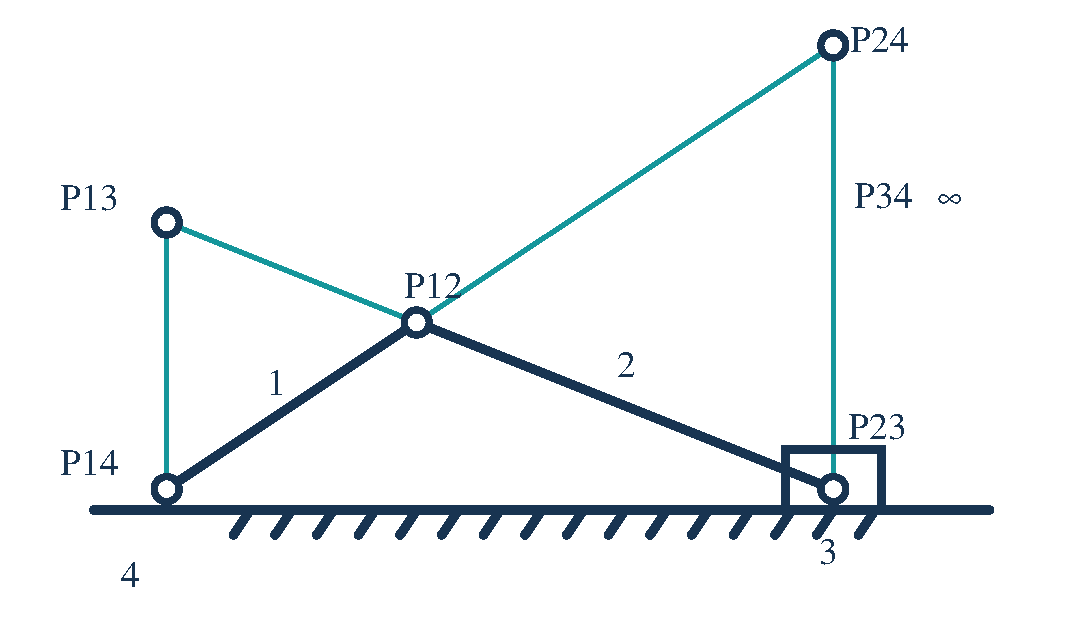
\includegraphics[width=.8\linewidth,height=8cm,keepaspectratio]{instant-center-vector.pdf}\end{center}


图 3-2 曲柄滑块机构瞬心构造（自绘，整理自 B091-01 第 7—8 页）。


\textbf{例题｜找出全部六个瞬心。} 图中 1 为曲柄、2 为连杆、3 为滑块、4 为机架。先找直接相连者：P14、P12、P23 分别在三个转动副，P34 位于垂直滑块导路的无穷远处。再用三心定理：P13 同时位于 P14—P34 和 P12—P23 两条线上；P24 同时位于 P14—P12 和 P23—P34 两条线上。分别作交点即可。构件数 N=4，瞬心数为 4$\times$3/2=6，恰好与清单一致。图中延长线的交点是瞬时位置，尺寸只为演示。


\textbf{边界与自检。} 若接触点存在相对滑动，能否仍把它当作两构件的瞬心？不能；应结合公法线和其他已知瞬心确定。若构形使所需直线平行或瞬心趋于无穷远，要按该位置的极限关系分析。B091-01 第 7—8 页提供基本关系与曲柄滑块例题，本图和步骤为重绘整理；原件第 2 页的考频分值只代表该材料的复习提示。


\needspace{12\baselineskip}


\subsection{本章复盘}

\begin{longtable}{p{7.51cm}p{7.51cm}}
\toprule
问题 & 三句话带走 \\

\midrule
\endhead
是什么 & 自由度表示机构独立运动参数的个数。 \\
为什么 & 低副和高副对构件运动施加不同数量的约束。 \\
边界 & 局部自由度、复合铰链和虚约束不能重复计数。 \\
\bottomrule
\end{longtable}

\section{四、螺旋传动}

\begin{center}
\includegraphics[width=.8\linewidth,height=8cm,keepaspectratio]{chapter-map-04.pdf}\end{center}


图 4-1 螺旋传动知识地图（自绘）。





\subsection{C-3403｜螺旋传动}
\label{c-3403}

在常用螺旋副模型中，自锁条件为螺旋升角小于当量摩擦角；实际振动、磨损等可能影响自锁。力与效率公式须根据螺纹类型、受力方向和摩擦假设选用，待与原资料核对。





\subsection{K-3409｜螺旋传动的力与效率}
\label{k-3409}

螺距 p 是相邻牙对应点的轴向距离，导程 P$_{h}$ 是同一螺旋线上转一周的轴向位移，线数为 n 时 P$_{h}$=np；中径 d$_{2}$ 上升角满足 tan $\lambda$=P$_{h}$/($\pi$d$_{2}$)。轴向载荷 F、矩形螺纹摩擦角 $\rho$、忽略其他摩擦时，提升力矩 T=F d$_{2}$ tan($\lambda$+$\rho$)/2，效率 $\eta$=tan $\lambda$/tan($\lambda$+$\rho$)。非矩形螺纹按牙型斜角 $\beta$ 引入当量摩擦因数 f$_{v}$=f/cos $\beta$ 和当量摩擦角 $\rho$$_{v}$=arctan f$_{v}$；以上力矩和效率中的 $\rho$ 改用 $\rho$$_{v}$。公式适用于所设稳态正行程模型，若题目包括端面摩擦须另计。


\textbf{反行程与临界条件。} 按 S1 第 3 页的阻力方向，矩形螺纹反行程阻力矩为 $T_{\mathrm{rev}}=Fd_2\tan(\lambda-\rho)/2$。在该理想摩擦模型下，$\lambda>\rho$ 时载荷可反驱；$\lambda=\rho$ 是临界，$\lambda<\rho$ 才有自锁余量。非矩形牙用当量摩擦角代替 $\rho$；支承面摩擦和振动等实际因素另作判断。





\subsection{K-3515｜螺旋副：转一圈，前进多少？}
\label{k-3515}

\textbf{第一讲 01:14、16:06。} 先按上一章的方法处理局部自由度、复合铰链和虚约束。螺杆和螺母组成螺旋副；固定螺杆使其只能转、限制螺母转动，螺母就沿轴移动。大径、小径分别对应牙形的外、内边界；中径处牙厚等于槽宽。轴向截面内两牙侧夹角为牙形角，牙侧与轴线垂线的夹角为牙形斜角，对称牙形取半牙形角。


\textbf{30:10、41:33。} 把中径圆柱展开，一圈的底边是 $\pi$d$_{2}$，高是导程 L=np。因此 tan$\lambda$=L/($\pi$d$_{2}$)，使用导程后不再乘线数。将矩形牙等效为斜面上的重物，正压力垂直斜面，摩擦力阻碍相对滑动。匀速提升轴向力 F 所需圆周力为 F tan($\lambda$+$\rho$)，乘中径半径即得扭矩 T。一圈有用功 FL，输入功 2$\pi$T。自锁指轴向载荷不能自行反驱，仍可施加反向扭矩使其下降。


\textbf{第二讲 01:05、13:15。} 以 $\varphi$ 表示当量摩擦角，提升效率 $\eta$=tan$\lambda$/tan($\lambda$+$\varphi$)。能由载荷反驱时，反行程效率为 tan($\lambda$$-$$\varphi$)/tan$\lambda$。$\lambda$=$\varphi$ 是临界，要求可靠自锁应留余量。常用小升角范围内增加导程提高效率，同时减小自锁余量。矩形牙侧倾角为零；梯形牙方便加工，常用于传动；普通三角牙多用于紧固，管螺纹用于管路连接。千斤顶重在传力，机床进给丝杠重在传递位移，调整螺钉重在微调。


\textbf{差动螺旋的符号约定（S1 第 3—4 页）。} 对原图所示结构，螺杆转角为 $\varphi_1$、两段有符号导程为 $P_{hA}$、$P_{hB}$ 时，螺母 2 的位移 $l_2=(P_{hA}-P_{hB})\varphi_1/(2\pi)$。此图约定右旋导程为正、左旋为负；从左向右看，顺时针转角为正；位移正值向右、负值向左。例如两段均右旋，导程分别为 4 mm、3 mm，顺时针转一圈，则螺母向右移动 1 mm。换用其他观察方向或机构布置时，应重新规定方向并推导，不能直接照搬符号。


\textbf{作业讲评 48:31—49:50｜从螺纹圆周力换到手柄力。} 提升时先用轴向载荷、升角和当量摩擦角求驱动力矩 T，再由手柄有效力臂 l 求垂直施力 F手=T/l。手柄越长，同一扭矩所需手力越小。仅考虑螺纹摩擦时 $\eta$=tan$\lambda$/tan($\lambda$+$\varphi$)，计算器的角度模式要与升角、当量摩擦角的单位一致。


\needspace{12\baselineskip}


\subsection{本章复盘}

\begin{longtable}{p{7.51cm}p{7.51cm}}
\toprule
问题 & 三句话带走 \\

\midrule
\endhead
是什么 & 螺旋副把转动与轴向移动联系起来。 \\
为什么 & 中径圆柱展开后，可由导程和摩擦建立力矩关系。 \\
边界 & 摩擦角、受力方向及端面摩擦不同时不能照搬公式。 \\
\bottomrule
\end{longtable}

\section{五、丝杆形式}

\begin{center}
\includegraphics[width=.8\linewidth,height=8cm,keepaspectratio]{chapter-map-05.pdf}\end{center}


图 5-1 丝杆形式知识地图（自绘）。


用户笔记中的“丝杆形式”与杆长条件、死点和行程速比是否指同一内容尚待确认。下列四杆机构材料按既有笔记保留，不断言它就是用户所称的丝杆形式；螺旋传动另见第四部分。





\subsection{C-3404｜平面连杆机构（用户笔记“丝杆形式”，待核对）}
\label{c-3404}

用户所写“最大＋最小＜其他两数之和”、死点、行程和 K 指向平面四杆机构，具体标题需核对原件。对于满足杆长和条件的铰链四杆机构，最短杆与最长杆长度之和小于或等于其余两杆长度之和是曲柄存在的必要杆长条件；还须根据机架选择判断具体机构类型。压力角与传动角互余时，压力角越小、传动角越大，通常越有利于传力。死点须结合主动件和机构位置判断。行程及 K 的具体定义需依题目和原资料确定。





\subsection{K-3410｜曲柄摇杆行程速比}
\label{k-3410}

匀速曲柄驱动时，行程速比系数 K=(180°+$\theta$)/(180°$-$$\theta$)，$\theta$ 为极位夹角。反求 $\theta$=180°(K$-$1)/(K+1)。例如 K=1.4，$\theta$=30°；这是资料 2 选择题第 6 题对应结果，答案页给 A，具体选项符号仍需原图核对。$\theta$=0 时 K=1，无急回。





\subsection{K-3436｜曲柄摇杆机构：极位和行程图解}
\label{k-3436}

【来源】资料 1 第 4—5 页的极位与行程速比；以下尺寸和图为自编。机架 AD=3.5，曲柄 AB=1，连杆 BC=3，摇杆 DC=2，长度单位一致。摇杆极位发生在 AB 与 BC 共线，即 AC=AB+BC=4 或 AC=BC$-$AB=2。\textbf{绘图步骤}：\textcircled{1}按比例画机架 AD；\textcircled{2}以 D 为圆心、DC=2 为半径画摇杆端点轨迹；\textcircled{3}分别以 A 为圆心、4 和 2 为半径画弧，与摇杆轨迹相交得 C$_{1}$、C$_{2}$（同一装配支路取同侧交点）；\textcircled{4}按共线关系确定 B$_{1}$、B$_{2}$；\textcircled{5}连接 DC$_{1}$、DC$_{2}$，夹角 $\psi$ 即摇杆角行程。若从动件为滑块，行程为两极限位置沿导路的距离，不是摇杆角度。


\begin{center}
\begin{tikzpicture}[scale=1.15, line cap=round, line join=round]
\coordinate (A) at (0,0); \coordinate (D) at (3.5,0);
\coordinate (C1) at (3.4643,1.9997); \coordinate (C2) at (1.75,.9682);
\coordinate (B1) at (.8661,.4999); \coordinate (B2) at (-.875,-.4841);
\draw[line width=1.2pt] (A)--(D); \draw[thick,navy] (A)--(B1)--(C1)--(D);
\draw[thick,tealaccent,dashed] (A)--(B2)--(C2)--(D);
\draw[gray,densely dotted] (A) circle (1); \draw[gray,densely dotted] (C2) arc (151:91:2);
\foreach \p/\n/\pos in {A/A/below,D/D/below,C1/$C_1$/above,C2/$C_2$/above,B1/$B_1$/below,B2/$B_2$/below} {\fill (\p) circle (1.8pt);\node[\pos] at (\p) {\n};}
\node[align=left,font=\small] at (2,-1.05) {实线：$AC_1=4$；虚线：$AC_2=2$};
\end{tikzpicture}
\end{center}


【解】在三角形 ADC$_{1}$、ADC$_{2}$ 中分别用余弦定理求摇杆与机架夹角。令两角为 $\gamma$$_{1}$、$\gamma$$_{2}$，则 cos $\gamma$$_{1}$=(AD$^{2}$+DC$^{2}$$-$AC$_{1}$$^{2}$)/(2·AD·DC)=1/56，cos $\gamma$$_{2}$=(AD$^{2}$+DC$^{2}$$-$AC$_{2}$$^{2}$)/(2·AD·DC)=7/8。因此 $\psi$$\approx$88.98°$-$28.96°=60.02°。图中的 $\psi$ 是从动摇杆的角行程，\textbf{不同于}用于急回计算的极位夹角 $\theta$。曲柄两极限位置的夹角需按曲柄实际转动方向确定，再求 $\theta$ 和 K=(180°+$\theta$)/(180°$-$$\theta$)。


【自检】已知 K=1，$\theta$ 是多少？答：$\theta$=0°，两行程平均速度相等；这不代表从动件在行程中匀速。





\subsection{K-3516｜平面连杆机构：固定哪根杆？}
\label{k-3516}

\textbf{第二讲 25:44、38:22。} 低副面接触，便于润滑和承载；铰链间隙会累积成输出误差。四根杆中先标机架，对面是连杆，两旁是连架杆。能整周转的连架杆叫曲柄，只能来回摆的叫摇杆。曲柄摇杆可把电机旋转变为筛体摆动，双曲柄可使机车两车轮联动，双摇杆的两连架杆均摆动。曲柄滑块以移动副实现往复直线运动。设最短杆 s、最长杆 l，其余 p、q；一般铰链四杆满足 s+l<p+q 时，固定最短杆为双曲柄，固定其邻杆为曲柄摇杆，固定其对杆为双摇杆；等号对应可能出现共线的临界情况。


\textbf{连杆机构有什么取舍？} 原资料 B091-02 第 3 页指出，低副接触面积较大，通常便于承载和润滑；合理组合杆件也能得到不同的连杆轨迹和运动变换。与此同时，多个运动副的间隙和制造误差可能累积，惯性载荷及其平衡也需考虑。具体传动效率、精度和适用速度取决于结构与工况，不能只按机构名称一概判断。


\textbf{曲柄与周转副不是同一个概念。} 能绕机架整周转动的连架杆称曲柄，只能在一定范围往复摆动的连架杆称摇杆；周转副和摆转副则描述转动副中两构件是否能相对整周转动。前一组名称说的是杆的运动能力，后一组说的是运动副的相对运动能力。该区分整理自 B091-02 第 4 页，判断时仍须结合整个机构的约束。


\textbf{四杆专题 01:11｜用三角形看整转条件。} 设固定铰链为 A、D，想让 AB 整转。曲柄端 B 绕 A 转一周时，到 D 的距离从 |AD$-$AB| 变到 AD+AB。另两杆 BC、CD 必须始终能接成三角形 BCD，因此最远处须满足 AD+AB$\le$BC+CD，最近处须满足 |AD$-$AB|$\ge$|BC$-$CD|。等号允许三点共线。这个画圆的办法解释了为何只看杆能否装在一起，还不能断定它能整转。


\textbf{12:42｜先比杆长，再看机架。} 对可装配、最短杆唯一的一般铰链四杆，若 s+l>p+q，固定任何一杆均为双摇杆；若 s+l<p+q，按上段三种机架位置判型。s+l=p+q 是临界情形，应检查共线位置及通过方式。整理自编例：沿环路 AB、BC、CD、DA 分别长 20、45、50、55 mm。20+55<45+50，固定 AB 为双曲柄；固定 DA 或 BC，AB 为曲柄；固定 CD 为双摇杆。由此可见，最短杆作机架是双曲柄的一种判据，邻杆作机架也可以有曲柄。


\textbf{27:10｜辨认机构的演化。} 先标出每处相对运动，再数转动副和移动副。四个转动副的铰链四杆，若将摇杆端的圆弧导引改成直线导引，可演化为三转一移的曲柄滑块；扩大曲柄销并保留偏心距，可得到偏心轮机构；含两个移动副的四杆机构可形成双滑块机构。改变固定构件也能得到不同用途的机构。识图时，盘做得再大，若轴心与盘心仍有偏心距，就应按两中心间的距离识别等效曲柄长。


\textbf{39:34｜从两个极限位置读出急回。} 匀速转动曲柄 AB，当 AB 与 BC 拉直或折叠共线时，摇杆 CD 分别到达两个摆动端点。画下两次曲柄的位置，沿给定转向从一个端点走到另一个，再走回来。若两段曲柄转角为 180°+$\theta$ 和 180°$-$$\theta$，较大转角用时较长。摇杆往返扫过同一个摆角，所以 K=回程平均角速度大小/工作行程平均角速度大小=工作行程时间/回程时间（约定工作行程较慢）。自编读图例：两段转角为 210° 和 150°，$\theta$=(210°$-$150°)/2=30°，K=210/150=1.4。$\theta$ 越大，急回越明显；$\theta$=0 时两段各占半圈。作图时把 $\theta$ 标在曲柄侧，把摇杆摆角标在 D 点，避免混用。


\textbf{传力专题 01:10｜先标谁在驱动。} 沿用 A、D 为固定铰链，AB 为曲柄，BC 为连杆，CD 为摇杆。先按杆长和机架位置确认 AB 能整转，再画 AB 与 BC 拉直、折叠的两个位置。若由 AB 匀速驱动，CD 在这两处瞬时角速度为零，随后反向；两次换向之间的平均速度用于判断急回。


\textbf{11:46｜把找极位的方法迁移到其他机构。} 极位夹角 $\theta$ 可由两段曲柄转角之差的一半求得，行程速比系数 K=(180°+$\theta$)/(180°$-$$\theta$)。$\theta$=0 时机构仍往复运动，只是两行程时间相等。对心曲柄滑块的导路通过曲柄转轴，两次极位间曲柄各转半圈；偏置时应画曲柄与连杆两次共线的位置，沿实际转向读角。对摆动导杆机构，从导杆固定铰链向曲柄销的圆轨迹作两条切线，切点就是导杆摆到两端时的曲柄销位置。


\textbf{24:21｜最小传动角怎样算。} 在忽略摩擦、惯性且连杆为二力杆的模型中，力沿 BC，摇杆端 C 的速度垂直于 CD。压力角 $\alpha$ 取力的作用线与速度方向所成的锐角或零角；传动角 $\gamma$ 取 BC 和 CD 两直线间较小的夹角（可达 90°），两者互余。传给摇杆的力矩大小为 F·CD·sin$\gamma$，同样的连杆力在 $\gamma$ 较小时产生的力矩较小。求全周期最小值时，画 \textbf{AB 与机架 AD 共线} 的两个位置，此时 BD 分别取 |AD$-$AB| 和 AD+AB。在三角形 BCD 中，两次用 cos$\angle$BCD=(BC$^{2}$+CD$^{2}$$-$BD$^{2}$)/(2·BC·CD) 求角；若得到钝角就取补角，最后在两个结果中选小值。注意此处的共线杆件与求摇杆极位时不同。


\textbf{滑块能否连续运动与传动角。} 对理想偏置曲柄滑块，设曲柄半径 r、连杆长 l、导路到曲柄轴心的垂直距离为 |e|。若 l>r+|e|，曲柄销转一周时到导路的最大垂直距离仍小于连杆长，因此几何上可保持同一滑块装配支路；等号会出现边界构形，实际装配还须检查干涉和副的行程。对心时 e=0，条件简化为 l>r。B091-02 第 6 页给出对应判据；该页对导杆机构的“任何条件”应理解为其理想示意模型，实际仍需满足尺寸、行程和干涉要求。


\textbf{比较滑块与导杆的传力。} 对图示理想曲柄滑块，在忽略摩擦和惯性、连杆近似二力杆且曲柄能连续整转时，可在曲柄垂直导路的两个位置比较传动角；因为此时曲柄销到导路的垂直距离达到候选极值。对原资料所示的理想无摩擦导杆，接触力与导杆上接触点速度同向，压力角为 0°、传动角为 90°；实际摩擦和间隙会改变力的方向。原资料将极位夹角称为“锐角”，该说法适用于其示例，不应据此排除其他非退化角度；应按题给角度定义和实际位置判断。


\textbf{36:46｜同一个姿态，换主动件再判死点。} AB 与 BC 共线时，若摇杆 CD 主动，连杆力的作用线穿过曲柄轴心 A，力臂为零，无法靠该力在这一瞬间启动曲柄；此时对输出曲柄的传动角为零。换成曲柄主动，同一姿态只是摇杆换向的极位，曲柄可以继续转。多套机构可把死点错开，例如蒸汽机车两侧曲柄错相，使另一侧仍能提供转矩。起落架撑杆则可利用接近共线或越过中心的布置配合止挡锁定。死点取决于构件位置和驱动方向；螺旋副的摩擦自锁取决于升角与当量摩擦角，即使没有几何死点，轴向载荷也可能无法反驱。


\textbf{尺度综合课 01:10｜先标端点在哪里运动。} 摆动导杆绕固定铰链 D 摆动，曲柄销绕固定中心 A 走圆；从 D 向圆作两条切线，就是导杆的两个极限方向。曲柄滑块的滑块销沿导路直线运动，到极位时曲柄与连杆共线。先根据题目指定的输出选机构，再用行程、摆角、速比等要求求杆长和固定铰链位置，这一步称尺度综合。画完还要沿同一装配分支检查能否连续运动、传动角是否合适、构件是否干涉。


\textbf{16:25｜图解设计：把条件画成轨迹，交点才是候选轴心。} 曲柄匀速、工作行程较慢时，由 K 求极位夹角 $\theta$=180°(K$-$1)/(K+1)。以下是按课堂主题补充的通用作法，符号以本段为准。


\begin{longtable}{p{7.51cm}p{7.51cm}}
\toprule
给定机构及条件 & 作图与回验 \\

\midrule
\endhead
曲柄摇杆：已定位摇杆端点的两个极位 C$_{1}$、C$_{2}$，并给 K & 以 C$_{1}$C$_{2}$ 为弦，作使 $\angle$C$_{1}$AC$_{2}$=$\theta$ 的圆弧轨迹（$\theta$>0）。再用题给的机架长度或轴心位置限制选 A。极位时 AC 的两种长度分别为连杆长加、减曲柄长，故曲柄长为两距离之差的一半，连杆长为两距离之和的一半。回验机架、整转条件和转向。 \\
摆动导杆：已知 K、机架长 AD=d & 两条极限导杆线的夹角为 $\theta$。在 D 画出两条射线，在其内角平分线上取 DA=d，从 A 向射线作垂线。垂足是极位曲柄销，垂距就是曲柄半径 r=d sin($\theta$/2)。 \\
偏置曲柄滑块：已知行程 h、偏距 e，并指定 K & 在导路上取 C$_{1}$、C$_{2}$，相距 h；作与导路距离为 e 的平行线，作为曲柄轴心轨迹。再与满足极位夹角的圆弧相交选 A，按两段 AC 的和、差各除以二求杆长。只给 h、e 时通常还有多组解，需要 K 或另一尺寸。对心且 K=1 时，两极位和轴心共线，曲柄长 h/2，连杆长另选。 \\
\bottomrule
\end{longtable}

\textbf{辅助圆的角度与退化边界（B091-02 第 24 页）。} 对已确定的两个极位 C1、C2，先由 K 求 $\theta$，再找满足 $\angle$C1AC2=$\theta$ 的候选轴心 A。设弦长 c=|C1C2|，当 0<$\theta$<180° 时，辅助圆半径 R=c/(2sin$\theta$)，圆心在弦的中垂线上，距弦中点的有向距离与 (c/2)cot$\theta$ 对应。图形关于弦有对称分支；应在能给出所需圆周角的弧上选 A，并排除 C1、C2 及使两段 AC 等长、导致曲柄长度为零的退化选择。


原资料用 90°$-$$\theta$ 作三角形底角，该画法直接适用于 0<$\theta$<90° 的示意；$\theta$=90° 时辅助圆以弦为直径，$\theta$>90° 时不能照搬负角，应改用圆周角条件并选择正确的圆弧。$\theta$=0 即 K=1 时圆半径趋于无穷大，轴心及两个极位需按共线极限单独处理。无论哪种方法，取点后均须回验杆长、转向、极位和同一装配支路；仅在圆上取点并不保证方案可用。


\textbf{自编图解｜摆动导杆的两个极位}


\begin{center}\begin{tikzpicture}[scale=.83,thick,>=stealth,font=\small]
\draw (0,0) node[left]{D} -- (6,0) node[below right]{A};
\draw[tealaccent] (6,0) circle (3);
\foreach \y in {-2.598,2.598}{\draw[navy] (0,0)--(4.5,\y)--(6,0);\fill (4.5,\y) circle(2pt);}
\draw[->] (1.3,-.75) arc(-30:30:1.5);
\node at (2,0.35){$\theta/2$};\node[right] at (6,2){曲柄销轨迹};
\end{tikzpicture}\end{center}


从导杆铰链 D 看，极限位置是上下两条切线。切点处半径垂直于导杆；固定中心距 DA 是直角三角形的斜边。


\needspace{18\baselineskip}


\textbf{自编图解｜偏置滑块：先画两条平行线}


\begin{center}\begin{tikzpicture}[scale=.83,thick,>=stealth,font=\small]
\draw[->] (-1,0)--(9,0) node[right]{滑块导路};
\draw[dashed] (-1,2)--(9,2) node[right]{轴心轨迹};
\draw[<->] (-.5,0)--node[left]{$e$}(-.5,2);
\draw[navy] (2,0) node[below]{$C_1$}--(0,2) node[above]{A}--(7,0) node[below]{$C_2$};
\draw[<->] (2,-.6)--node[below]{$h$}(7,-.6);
\end{tikzpicture}\end{center}


两条实线表示两次共线极位时轴心到滑块销的距离。用较大距离减较小距离得到两倍曲柄长；它通常不等于导路上的行程 h。





\subsection{K-3556｜急回、死点和三位置反求轴心}
\label{k-3556}

\textbf{同样有急回，用途要看工作过程。} B091-02 第 17 页举牛头刨床：工作行程较慢以适应切削，非工作行程较快以缩短空程。该页以颚式破碎机为例，称较快的工作行程有助于击碎矿石，较慢的回程有助于碎料落下。这里的快慢是针对具体机构和工况的示例，不能将某一种安排推广到所有设备。


\textbf{死点可以避免，也可以利用。} 缝纫机或内燃机可利用飞轮储存的动能帮助机构通过瞬时死点；多组机构也可错开死点。夹具及起落架撑杆可采用接近共线或越过中心的布置，并结合止挡或锁定装置维持工作位置。是否可靠锁定还取决于结构、载荷和装置，不是所有共线姿态都会自行锁住。


\textbf{已知连杆的三个位置，反求固定铰链。} 已知同一根连杆 BC 的三个对应位置 B1C1、B2C2、B3C3，四杆中 AB、CD 长度固定。因为 B1、B2、B3 都到 A 等距，A 是这三个点所确定圆的圆心；D 同理。步骤见下表。


\begin{longtable}{p{7.51cm}p{7.51cm}}
\toprule
步骤 & 为什么 \\

\midrule
\endhead
连 B1B2、B2B3，分别作中垂线 & 等距点 A 必在每条弦的中垂线上 \\
取两条中垂线的交点 A & 得到满足 AB1=AB2=AB3 的候选固定铰链 \\
对 C1、C2、C3 重复上述作法，求 D & 保证 DC1=DC2=DC3 \\
连成机构并回验三个位置 & 还须检查 BC 各位置长度一致、装配支路、整转和干涉 \\
\bottomrule
\end{longtable}

若同一组的三个点共线且互不相同，无法确定有限的圆心；若点重复或近乎共线，解可能不唯一或对误差很敏感。B091-02 第 25 页提供中垂线作图，题册另给出自编坐标例子。


\needspace{12\baselineskip}


\subsection{本章复盘}

\begin{longtable}{p{7.51cm}p{7.51cm}}
\toprule
问题 & 三句话带走 \\

\midrule
\endhead
是什么 & 本部分按原笔记中的杆长、死点和行程内容讲平面四杆机构。 \\
为什么 & 机构类型取决于杆长关系和固定杆的选择。 \\
边界 & “丝杆形式”与此部分是否同义尚未确认。 \\
\bottomrule
\end{longtable}

\section{六、凸轮}

\begin{center}
\includegraphics[width=.8\linewidth,height=8cm,keepaspectratio]{chapter-map-06.pdf}\end{center}


图 6-1 凸轮知识地图（自绘）。





\subsection{K-3418｜滚子凸轮作图（整理说明，参照资料 1 第 5—6 页与资料 2 第 4、11 页）}
\label{k-3418}

\begin{enumerate}
\item 
找固定凸轮中心、从动件导路和滚子中心；基圆通常以凸轮转动中心为圆心，半径取理论轮廓的最小向径，使用教材定义时核对其是否指理论廓线基圆。


\item 
用反转法把凸轮视为静止，让从动件导路相对凸轮反向转动，并按给定位移规律确定各时刻滚子中心。依次连接滚子中心得理论轮廓。


\item 
以理论轮廓上的滚子中心作滚子圆，其包络线为实际轮廓；作接触处公法线与从动件速度方向的夹角得压力角。偏置圆以凸轮中心为圆心、偏距为半径，导路与偏置圆相切。


\item 
检查推程、回程、远休止和近休止的位置与转向。外凸理论轮廓局部曲率半径必须足以容纳滚子半径，否则可能产生尖点或失真；曲率符号和内凹部分需要分别分析。



\end{enumerate}

自检：滚子半径变大时，理论轮廓是否自动改变？答：在给定运动规律与滚子中心轨迹不变的前提下不改变，但实际包络轮廓会改变。


\textbf{滚子半径与局部曲率。} 按 B091-03 第 13 页所示的局部偏移约定，外凸段的实际轮廓曲率半径为理论轮廓曲率半径减去滚子半径；相等时局部趋于尖点，滚子更大可能发生轮廓失真。内凹段在该局部约定下为两者相加。原页文字称“内凹型理论轮廓的滚子半径不会影响实际轮廓”，但同页公式又包含滚子半径；应理解为内凹段不存在上述外凸段的同一种尖点限制，而不是实际曲线完全不随滚子改变。以上是局部几何关系，完整轮廓还要检查其他位置和包络干涉。





\subsection{K-3424｜凸轮运动规律和原式勘误}
\label{k-3424}

【来源】资料 1 第 5—6 页，资料 3 第 1 页；以下式子经位移求导核对，凸轮角速度 $\omega$ 为常数，$\varphi$ 以弧度计。


推程角 $\delta$、推程 h。等速规律在 0$\le$$\varphi$$\le$$\delta$ 内：s=h$\varphi$/$\delta$，v=h$\omega$/$\delta$，a=0；起止点与休止段连接时速度突变，有刚性冲击。等加速等减速规律在前半段（0$\le$$\varphi$$\le$$\delta$/2）：s=2h$\varphi$$^{2}$/$\delta$$^{2}$，v=4h$\omega$$\varphi$/$\delta$$^{2}$，a=4h$\omega$$^{2}$/$\delta$$^{2}$；在后半段（$\delta$/2$\le$$\varphi$$\le$$\delta$）：s=h$-$2h($\delta$$-$$\varphi$)$^{2}$/$\delta$$^{2}$，v=4h$\omega$($\delta$$-$$\varphi$)/$\delta$$^{2}$，a=$-$4h$\omega$$^{2}$/$\delta$$^{2}$。中点位移为 h/2，两段加速度大小相等、方向相反。其加速度在起止和中点突变，有柔性冲击。简谐（余弦加速度）也有加速度跃变；摆线（正弦加速度）在与休止段连接时速度和加速度均连续，适合高速轻载。


\textbf{摆线规律的速度和加速度。} 令推程角为 $\delta$、凸轮匀角速度为 $\omega$、推程位移为 h，并设 u=$\varphi$/$\delta$。对 0$\le$u$\le$1，摆线推程的位移、速度和加速度可写为：


$s=h\left(u-\dfrac{\sin(2\pi u)}{2\pi}\right)$；$v=\dfrac{h\omega}{\delta}\left(1-\cos(2\pi u)\right)$；$a=\dfrac{2\pi h\omega^2}{\delta^2}\sin(2\pi u)$。


因此 $v_{\max}=2h\omega/\delta$，加速度的最大绝对值为 $2\pi h\omega^2/\delta^2$。这里 $\varphi$、$\delta$ 均以弧度计，$\omega$ 为常数；B091-03 第 7 页的图中将系数 2$\pi$ 近似写为 6.28。与休止段连接时，摆线规律在端点的速度和加速度均为零。


【审校】资料 1 第 5 页两段加速度分子印为 4h$\omega$，量纲和对速度求导均表明应为 4h$\omega$$^{2}$。资料 3 第 1 页称正弦加速度“刚性和柔性冲击”，与该运动规律及试卷第 5 题答案冲突，应为两者均无；本段按给定运动规律求导判断。


\textbf{课堂 00:52｜看图命名，按一周划分运动。} 先找机架、凸轮、从动件。凸轮按形状分盘形、移动、圆柱；从动件按接触端分尖顶、滚子、平底，按运动形式分直动、摆动。例如“盘形凸轮＋滚子＋沿导轨移动”可命名为滚子直动从动件盘形凸轮机构。位移图横轴为凸轮转角 $\varphi$，纵轴为从动件位移 s。常见一周依次为推程、远休止、回程、近休止，四段转角之和为 360°。行程 h 是最高与最低位移之差，休止段在位移图上是一段水平线。


\textbf{13:06｜从轮廓读运动，从运动画轮廓。} 给定从动件形式、导路和安装位置后，转动凸轮，逐角度记录从动件位置即可画出 s($\varphi$)。若凸轮匀速转动，$\varphi$ 用弧度、角速度为 $\omega$，则 v=$\omega$ ds/d$\varphi$，a=$\omega$$^{2}$ d$^{2}$s/d$\varphi$$^{2}$。位移图越陡，速度大小越大；斜率在接头处突然改变，就意味着速度突变。反过来，设计时先给定行程、各段转角和运动规律，再据此构造凸轮轮廓。


\textbf{25:19｜运动段接休止段时，先查速度，再查加速度。}


\begin{longtable}{p{4.86cm}p{4.86cm}p{4.86cm}}
\toprule
运动规律 & 位移、速度和加速度怎样变化 & 接头处及选用提示 \\

\midrule
\endhead
等速 & 位移为直线，运动段速度恒定 & 起止速度跳变，有刚性冲击，宜低速轻载 \\
等加速等减速 & 位移由两段抛物线连接，速度先线性增加再线性减小，加速度分段恒定 & 起止及中点加速度跳变，有柔性冲击，常用于中速轻载 \\
余弦加速度（简谐） & 位移按余弦函数平滑起落，速度呈半个正弦波 & 端点速度为零，但加速度与休止段不连续，有柔性冲击，常用于中速 \\
正弦加速度（摆线） & 加速度在推程内走完一个正弦周期，速度从零升高再降至零 & 端点速度和加速度均为零，按上述判据无刚性或柔性冲击，适于较高速；重载仍须校核接触强度 \\
\bottomrule
\end{longtable}

\textbf{36:23｜反转法画滚子直动从动件盘形凸轮。} 把凸轮想成静止，让机架和导路绕凸轮轴心按实际转向的反方向旋转。\textcircled{1}在位移图和反转图上标出同一组角度分点。\textcircled{2}每到一个分点，沿该位置的导路，从对应的零位滚子中心量出位移。\textcircled{3}顺次光滑连接滚子中心，得理论轮廓；以各中心画等半径滚子圆，外凸轮取圆族靠凸轮实体一侧的包络，得实际轮廓。\textcircled{4}以凸轮轴心为圆心、到理论轮廓的最短距离为半径画理论基圆；在题指定位置画理论轮廓法线，与直动从动件速度方向的锐夹角为压力角（也可为零）。组合运动规律应逐个检查接头的位移、速度和加速度，同时考虑加工与承载条件。


\textbf{轮廓设计课 00:57｜先把两张图的分点对齐。} 选定长度比例尺，依次标出推程、远休止、回程和近休止的起止角。把推程和回程各自分段，在位移图上读每个分点的位移，再按同样的角度、编号反向转动导路。若各段运动角不同，不能把一周直接分成四个相等区段。休止段保留恒定位移，最后检查推程末点是否到达全行程、回程末点是否回到零位。


\textbf{一周四段怎样对应到轮廓？} B091-03 第 9—11 页的示例依次安排推程 120°、远休止 60°、回程 90°、近休止 90°，合计 360°。以凸轮实际逆时针转动为例，反转图中导路按顺时针方向依次经过同样的角度；同一角度在位移图上读得 s，再从对应导路的零位量取。对心尖顶可直接连接尖顶位置，偏置尖顶要先画偏距圆切线，滚子则先连接中心轨迹再作实际包络。题册给出使用这组角度的自编数值示例；其数值和回程曲线不冒充原页已给数据。


\textbf{12:00｜看接触端决定怎样连线，看偏置决定从哪条线量。} 尖顶的各个尖端位置直接连成实际轮廓；滚子先连中心轨迹，再沿公法线向凸轮实体侧偏移一个滚子半径，等价于取滚子圆族的包络。直接从各点的向径减去滚子半径通常会画错。平底从动件在各分点画出平底工作线，取这一族直线的包络。偏置是导路相对轴心的位置关系，可与尖顶或滚子组合：以偏距为半径画偏距圆，反转后的各导路与它相切，沿相应切线从反转后的零位量位移。


\textbf{28:16｜用压力角解释推杆为什么会卡住。} 忽略接触摩擦时，接触力沿公法线。压力角 $\alpha$ 是公法线与从动件运动方向所成的锐角（可为零）。直动推杆受正压力 N，沿导路的分力为 N cos$\alpha$，侧向分力为 N sin$\alpha$。$\alpha$ 越大，同样的正压力能提供的推力越小，导路侧压力越大。考虑导路摩擦时可能卡滞或自锁，不能单凭一个角度断定自锁。对心直动尖顶或滚子机构可用 tan$\alpha$=|ds/d$\varphi$|/(r$_{0}$+s) 核算，$\varphi$ 用弧度，r$_{0}$ 为理论基圆半径；偏置机构要按实际导路和法线量角。


\textbf{偏置与压力角的关系。} B091-03 第 12 页给出偏置直动从动件的一种符号约定：$\tan\alpha=\dfrac{|\mathrm{d}s/\mathrm{d}\varphi\pm e|}{s+\sqrt{r_b^2-e^2}}$。这里 e 是偏距，$r_b$ 是理论基圆半径，s 从基圆对应位置起量，$\varphi$ 以弧度计；分子符号取决于偏置方向和凸轮转向，须先按图中的公法线确定。本式要求 $r_b>|e|$ 且所用导路线与基圆的交点、位移方向符合该模型；对心 e=0 时回到前述对心式。在固定运动规律及其余几何条件下增大基圆通常可降低该模型中的压力角，但也会增大机构尺寸；更改偏置或从动件类型后应分别回验推程和回程。


\textbf{凸轮应用课 33:35｜从动作要求选轮廓。} 例如自动送料需要“推出—等待—退回”，可以先把这些动作分配到一周转角，再由位移图作轮廓。凸轮、从动件与机架能组成紧凑机构，输出可为直动或摆动。凸轮与从动件形成高副，点或线接触使局部接触应力较高，设计时还要考虑磨损和轮廓加工。滚子中心轨迹是理论轮廓，实际接触面是滚子圆族的包络；尖顶从动件的两条轮廓重合。


\textbf{42:35｜怎样让从动件始终贴着凸轮？} 力封闭靠弹簧力或重力维持接触，高速时须检查从动件是否会脱离；形封闭靠几何形状限制运动，例如槽凸轮用槽的两侧轮廓约束滚子。读位移图 s($\varphi$) 时，从最低位到最高位的位移差是行程 h，发生这段运动所占的转角是推程角；高位水平段占远休止角，下降段占回程角，低位水平段占近休止角。总转角为一周。滚子盘形凸轮按本课理论轮廓量基圆半径：以轴心为圆心，找理论轮廓离轴心最近处。


\textbf{自编图解｜滚子接触处的三条线}


\begin{center}\begin{tikzpicture}[scale=.83,thick,>=stealth,font=\small]
\draw[navy] (-3,0)--(3,0) node[right]{实际轮廓局部切线};
\draw[dashed] (-3,1)--(3,1) node[right]{理论轮廓局部切线};
\draw[tealaccent] (0,1) circle(1);\fill (0,0) circle(2pt) node[below left]{接触点};\fill (0,1) circle(2pt);
\draw[->] (0,1)--(0,3) node[above]{公法线};\draw[->] (0,1)--(1.6,3) node[right]{推杆速度};
\draw (0,1.85) arc(90:51:.85);\node at (.35,2.2){$\alpha$};
\end{tikzpicture}\end{center}


图示取接触附近的切线近似。滚子半径沿公法线连接中心和接触点；压力角从公法线量到速度方向。


\needspace{12\baselineskip}


\subsection{本章复盘}

\begin{longtable}{p{7.51cm}p{7.51cm}}
\toprule
问题 & 三句话带走 \\

\midrule
\endhead
是什么 & 凸轮把轮廓形状转换为从动件的运动。 \\
为什么 & 位移规律与几何轮廓共同决定压力角和接触状态。 \\
边界 & 作图须区分理论与实际轮廓，并检查曲率边界。 \\
\bottomrule
\end{longtable}

\section{七、齿轮析}

\begin{center}
\includegraphics[width=.8\linewidth,height=8cm,keepaspectratio]{chapter-map-07.pdf}\end{center}


图 7-1 齿轮析知识地图（自绘）。


\textbf{衔接课 28:16、39:19｜按两轴的位置识别齿轮。} 齿轮靠轮齿啮合传递运动和转矩。定传动比圆齿轮副的转速关系准确，适合紧凑布置；制造和安装精度要求较高，长中心距会增大尺寸。


\begin{longtable}{p{7.51cm}p{7.51cm}}
\toprule
题图特征 & 类型、转向与用途 \\

\midrule
\endhead
两轴平行 & 直齿圆柱轮常用于一般减速；斜齿进入啮合较平稳，但有轴向力；人字齿两半旋向相反，可抵消轴向力。按同一观察方向，外啮合两轮反转，内啮合两轮同转，直齿和斜齿均可构成内啮合。 \\
一个齿轮与一排直线齿啮合 & 齿轮齿条把回转与直线运动互换，可由接触处的切向速度判齿条方向。 \\
两轴相交或交错 & 相交轴可用直齿或曲线齿等锥齿轮；交错轴可用交错轴斜齿轮或蜗杆副。对于空间轴，分别标轴向和转向箭头。 \\
节曲线为非圆形 & 非圆齿轮可按设计规律改变瞬时传动比，用于需要周期性变速的机构。 \\
\bottomrule
\end{longtable}

本节按用户目录原称“齿轮析”组织齿轮几何、受力和失效；具体称谓待核对。


\textbf{齿廓原理课 00:00｜在图上找相对速度瞬心。} 设两个定轴齿轮的中心是 O$_{1}$、O$_{2}$，轮齿当前在 K 点接触。根据三心定理，两轮相对机架的瞬心 O$_{1}$、O$_{2}$ 与两轮的相对瞬心 P 共线。两齿在 K 处保持接触，法向速度相等，相对滑动只能沿公切线，因此 P 同时在 K 处的公法线上。画连心线，再画接触点公法线，交点 P 就是节点。课堂摘要的“水星”“三星定律”依此几何关系释读为“瞬心”“三心定理”。


\textbf{15:05｜为什么渐开线能保持传动比？} P 点处两轮速度相等，故 |$\omega$$_{1}$/$\omega$$_{2}$|=O$_{2}$P/O$_{1}$P。即使接触点 K 不断移动，只要公法线始终通过连心线上的同一定点 P，传动比就恒定。能配合实现给定传动规律的一对齿廓称为共轭齿廓。把一根绷紧的线从基圆上展开，线端画出的曲线就是渐开线；展开长度等于基圆上相应的弧长。齿廓上任一点的法线都与基圆相切，所以一对渐开线轮齿在同一侧啮合时，接触公法线始终是两基圆的同一条公切线。无滑动指发生线沿基圆展开的过程；实际轮齿在节点以外通常既滚动又滑动。


\textbf{26:54｜同一齿廓上，各点压力角不同。} 在 K 点画出齿廓法线，再画出垂直于 O$_{1}$K 的速度方向，两者夹角为该点的压力角 $\alpha$$_{k}$。由基圆半径 r$_{b}$ 与法线垂直得到 cos$\alpha$$_{k}$=r$_{b}$/O$_{1}$K。基圆上压力角为零，沿齿廓向外逐渐增大。齿条可看作分度圆半径趋于无穷大的极限，渐开线齿廓相应变为直线。分度圆用于规定单轮尺寸；节圆由两轮实际啮合时的节点确定。


\textbf{38:18｜从一个齿距算出整轮尺寸。} 在分度圆上量相邻同侧齿廓间的弧长 p，等于一个齿厚和一个齿槽宽之和。z 个齿距绕成一圈，故 zp=$\pi$d。定义模数 m=p/$\pi$，就得到 d=mz。常见标准直齿轮取分度圆压力角 $\alpha$=20°，基圆直径 d$_{b}$=d cos$\alpha$。按标准全齿高、无变位外齿轮计算，齿顶高 h$_{a}$=h$_{a}$* m，齿根高 hf=(h$_{a}$*+c*)m，其中 c* 是顶隙系数。取 h$_{a}$*=1、c*=0.25 时，齿根高为 1.25m。自编速算：m=2 mm、z=30 时，分度圆直径 60 mm，齿顶圆直径 60+2$\times$2=64 mm，齿根圆直径 60$-$2$\times$2.5=55 mm。


\textbf{啮合条件课 01:01｜中心距变了，为何速比仍相同？} 对一对仍能正常啮合的渐开线外齿轮，啮合线是两基圆的内公切线。两轮沿公法线的速度分量相等，故 |$\omega$$_{1}$|r$_{b}$$_{1}$=|$\omega$$_{2}$|r$_{b}$$_{2}$。移动一根轴不会改变基圆半径，所以传动比大小仍为 r$_{b}$$_{2}$/r$_{b}$$_{1}$=z$_{2}$/z$_{1}$，两外齿轮转向相反。这称为渐开线传动的中心距可分性。


\textbf{12:30｜画出真正参加工作的那段啮合线。} 画两中心和基圆，作工作侧的内公切线，与连心线交于节点 P。工作啮合角 $\alpha$${}^{\prime}$ 是啮合线与两节圆在 P 处公切线的锐夹角。固定安装时，接触点沿啮合线移动，$\alpha$${}^{\prime}$ 保持不变；另取中心距 a${}^{\prime}$ 后，应重新计算 cos$\alpha$${}^{\prime}$=(r$_{b}$$_{1}$+r$_{b}$$_{2}$)/a${}^{\prime}$。在啮合线上标两齿顶圆的交点，正常无干涉时，两交点间是实际啮合段。中心距增大通常使工作啮合角增大、实际啮合段缩短。判断能否继续传动，还要检查接触范围、重合度和干涉。


\textbf{23:30｜先验能否配对，再算转速。} 前一对齿和后一对齿沿啮合线的间距必须一致，这个距离叫基节 p$_{b}$（直齿轮的法向齿距），p$_{b}$=$\pi$m cos$\alpha$。标准渐开线直齿圆柱齿轮的配对条件是两轮模数相等、分度圆压力角分别相等。自编例：m=2 mm，$\alpha$=20°，z$_{1}$=20，z$_{2}$=40。标准安装中心距 a=m(z$_{1}$+z$_{2}$)/2=60 mm，各轮节圆与自身分度圆重合。若改为 61 mm 且仍正常啮合，则 cos$\alpha$${}^{\prime}$=60cos20°/61，$\alpha$${}^{\prime}$约为 22.4°；输入轮转两圈，输出轮仍反向转一圈。分度圆由单轮参数确定，节圆随安装条件确定。


\textbf{34:07｜再验下一对齿能否及时接上。} 端面重合度 $\varepsilon$$\alpha$=实际啮合段长度/基节。同一对轮齿走完啮合段以前，下一对齿须已进入啮合。$\varepsilon$$\alpha$<1 时中间会断开，$\varepsilon$$\alpha$=1 是理想临界，工程上应大于 1。自编读数例：若实际啮合段为 9 mm、基节为 6 mm，则 $\varepsilon$$\alpha$=1.5，表示平均有 1.5 对齿同时工作。一个啮合周期内，一半时间为单对齿啮合，另一半为双对齿啮合。





\subsection{K-3411｜标准直齿圆柱齿轮尺寸}
\label{k-3411}

先看两根轴的位置，再选齿轮形式：平行轴可用外啮合、内啮合的直齿或斜齿圆柱齿轮；齿轮齿条可把转动与直线运动相互转换；人字齿由两侧相反旋向的斜齿组成。相交轴可用直齿或曲齿圆锥齿轮；交错轴可用交错轴斜齿轮或蜗杆蜗轮。具体选择还要看载荷、尺寸和速度。


齿轮机构可在较大范围内传递功率和速度，通常结构紧凑、传动比准确、效率和可靠性较高；但对制造安装精度有要求，成本较高，不适合两轴距离很远的场合，且单靠轮齿啮合一般没有过载保护。实际效率、寿命与载荷、润滑及轮型有关。


标准、正常齿制且未变位时，分度圆直径 d=mz，齿顶圆直径 d$_{a}$=m(z+2)，齿根圆直径 d$^{f}$=m(z$-$2.5)，基圆直径 d$_{b}$=d cos $\alpha$；标准中心距 a=m(z$_{1}$+z$_{2}$)/2。这里 m 为模数，z 为齿数，$\alpha$ 为分度圆压力角；齿顶高系数取 1、顶隙系数取 0.25。标准直齿外啮合配对需模数和压力角相同。例：m=2 mm、z=20、$\alpha$=20°，则 d=40 mm、d$_{a}$=44 mm、d$^{f}$=35 mm。直齿轮圆周力 F$_{t}$=2T/d，径向力 F$_{r}$=F$_{t}$ tan $\alpha$，单位应统一。


齿面点蚀对应接触疲劳校核，齿根折断对应弯曲疲劳校核。磨损、胶合和塑性变形也属于可能失效形式；具体设计次序取决于齿面硬度与工况。





\subsection{K-3425｜齿轮几何、受力与失效}
\label{k-3425}

【来源】资料 1 第 6—10、17—18 页，资料 3 第 2 页；其中强度设计公式为资料给出的特定简化公式，不替代题目或教材给定的系数。


渐开线由绷紧的发生线沿基圆滚动形成。发生线离开基圆的长度等于对应展开的基圆弧长；在基圆外一点，发生线既是该点渐开线的法线，也是基圆的切线，其切点是该点的曲率中心，发生线段长度是曲率半径。理想无摩擦啮合时，接触正压力沿公法线；考虑摩擦时总接触力不必沿该方向。基圆上压力角为零，向径增大时压力角增大。标准直齿轮分度圆上 p=$\pi$m，s=e=$\pi$m/2，h$_{a}$=m，h$^{f}$=1.25m，总齿高 2.25m，基圆齿距 p$_{b}$=$\pi$m cos$\alpha$。一对标准外啮合直齿轮在标准中心距、理想标准齿厚条件下，两分度圆分别与节圆重合，顶隙为 c*m、理论齿侧间隙为零；实际制造和润滑常需留侧隙。改变中心距时不应仍把分度圆与节圆视为同一圆。


斜齿圆柱齿轮的法面模数 m$_{n}$、端面模数 m$_{t}$ 关系 m$_{t}$=m$_{n}$/cos$\beta$，d=m$_{n}$z/cos$\beta$；标准中心距为 a=m$_{n}$(z$_{1}$+z$_{2}$) / (2cos$\beta$)。当量齿数 z$_{v}$=z/cos$^{3}$$\beta$。标准齿条刀具 $\alpha$=20°、齿顶高系数 1、无变位时，理论界限约为 17.10 齿；严格不根切需至少 18 齿，工程上常允许轻微根切而取 17 齿。根切是范成加工时齿根渐开线被刀具切去，变位等条件会改变判断。


由转矩 T 和分度圆直径 d 求圆周力大小 F$_{t}$=2T/d，直齿轮径向分力 F$_{r}$=F$_{t}$ tan$\alpha$，法向力 F$_{n}$=F$_{t}$/cos$\alpha$。主动轮所受圆周力与其啮合点圆周速度相反，从动轮同向；外啮合径向力指向各自轮心。【审校】资料 1 第 8 页文字把 F$_{t}$ 与 F$_{r}$ 的名称写反，公式下标与图示表明上面的命名。斜齿轮另有轴向力；资料第 10 页给出：右旋用右手、左旋用左手，四指沿该轮转向，主动轮受力轴向取大拇指方向，从动轮取相反方向；应结合轴的视角与接触力反作用核对。


【简化设计表达式】资料 1 第 8 页给直齿接触疲劳直径估算 d$_{1}$$\ge$76.6 [KT$_{1}$(u+1)/($\psi$d[$\sigma$]H$^{2}$u)]\textasciicircum{}(1/3)，弯曲估算 m$\ge$1.26 [KT$_{1}$YFS/($\psi$d z$_{1}$$^{2}$[$\sigma$]F)]\textasciicircum{}(1/3)。d$_{1}$、m 为 mm，T$_{1}$ 为 N·mm，许用应力为 MPa，u 为大轮与小轮齿数比，$\psi$d=b/d$_{1}$。资料第 9 页斜齿对应系数分别为 75.6 和 1.24；参数定义及原书适用条件须核对，用户称设计中的许用值选取不考，不据此认定强度校核不考。


失效：轮齿折断查弯曲疲劳；点蚀查接触疲劳；高速重载注意胶合，开式传动注意磨损，低速重载可发生塑性变形。硬齿面闭式传动常先按弯曲设计、再校核接触；具体题目以给定方法为准。


蜗杆蜗轮一般同旋向，蜗杆头数 z$_{1}$、蜗轮齿数 z$_{2}$ 时速比大小 z$_{2}$/z$_{1}$；啮合处蜗杆圆周力与蜗轮轴向力、蜗杆轴向力与蜗轮圆周力分别构成作用与反作用。大速比、运转平稳，但相对滑动较大，需注意效率、磨损及润滑。





\subsection{K-3440｜直齿轮和蜗杆受力：可执行判向步骤}
\label{k-3440}

画受力时先在同一视图标出轴线、啮合点和主动从动关系。 $\odot$ 表示指向观察者，$\otimes$ 表示指向纸内；它们是空间方向，换视角后必须重判。下表针对原资料的常见理想齿面受力模型：


\begin{longtable}{p{7.51cm}p{7.51cm}}
\toprule
啮合副 & 力的对应关系与判断 \\

\midrule
\endhead
平行轴外啮合直齿 & 一对轮在同一接触点的圆周力和径向力分别反向；理想直齿不产生轴向力。圆周力相对各自啮合点的运动方向：主动轮阻转、从动轮驱转。 \\
平行轴外啮合斜齿 & 另有轴向力，接触处两轮对应三个分量分别反向。对主动轮用旋向及转向判轴向力，再由作用与反作用确定另一轮。 \\
直交轴蜗杆蜗轮 & 蜗杆圆周力对应蜗轮轴向力，蜗杆轴向力对应蜗轮圆周力，两径向力相反；这些方向须在同一空间坐标中比较。 \\
直交轴直齿锥齿轮 & 两圆周力相反，一轮径向力与另一轮轴向力对应；按实际轴向和锥体小端、大端判断。 \\
\bottomrule
\end{longtable}

轴向力“相互抵消”只表示方向相反，合力还取决于大小；即使合力较小，也须核算各轴承载荷和相应力矩。齿面力在轴计算中可等效移至轴线，但必须加入相应力偶，不能丢掉力臂。


【来源】资料 1 第 8—10 页及资料 2 第 5、11 页；以下为整理说明。\textcircled{1}先在每根轴上标转速和主动、从动；\textcircled{2}确定啮合点的切向速度；\textcircled{3}主动轮所受圆周力与速度相反、从动轮同向；\textcircled{4}外啮合径向力指向各自轴心；\textcircled{5}斜齿轮由旋向、转速与主动从动关系判轴向力，两轮在接触处满足作用力与反作用力。蜗轮蜗杆两轴通常垂直，蜗杆的圆周力与蜗轮轴向力对应，蜗杆轴向力与蜗轮圆周力对应；作用力反向时应先画三维坐标，不能在不同投影视图中直接比较左右箭头。


【试卷第 29 题的已确认关系】1—2 为蜗杆蜗轮，3—4 为外啮合斜齿轮，5—6 为蜗杆蜗轮，7—8 为直齿锥齿轮；2 与 3、4 与 5、6 与 7 各为同轴。参考答案用箭头和斜线给出选定旋向及力的方向，见原件 S2 第 11 页；本节步骤帮助检查，但不同观察方向造成的正负号和全部箭头尚未独立复核，作答时仍以题图与三维受力分析为准。





\subsection{K-3517｜齿轮加工、失效与空间受力}
\label{k-3517}

\textbf{加工课 00:49、13:50。} 标准直齿圆柱齿轮正确啮合要求模数和压力角分别相等；连续传动还要看实际啮合线长度 B$_{1}$B$_{2}$ 与基节 p$_{b}$ 之比，即重合度 $\varepsilon$$\alpha$=B$_{1}$B$_{2}$/p$_{b}$；它是同时啮合齿对数的平均值。理想临界值为 1，工程上应大于 1 并留裕量。N$_{1}$N$_{2}$ 是两基圆公切线上的理论啮合线段，实际段还受两齿顶圆限制。仿形铣削逐槽分度，适合小批量；展成法让刀具与齿坯按啮合关系运动，由一系列刀刃位置包络出渐开线。齿轮插刀可加工合适的内齿轮，齿条插刀模拟齿条，滚刀连续展成，适合批量加工。


\textbf{25:37、38:02。} 画啮合线与齿坯基圆的切点，再标刀具齿顶线与啮合线的交点；交点越过极限啮合点时，刀尖会再切去已形成的齿根渐开线。根切削弱齿根并缩短有效齿廓。增加齿数或让齿条刀具远离齿坯中心作正变位可减轻根切。标准齿条刀具的理论界限为 z$\ge$2h$_{a}$*/sin$^{2}$$\alpha$；$\alpha$=20°、h$_{a}$*=1 时约为 17.10，整数严格满足应取 18 或以上，17 是允许轻微根切的常用工程值。变位还须兼顾齿顶厚、配对中心距和重合度。


\needspace{16\baselineskip}


\textbf{失效怎么区分？} 从现象和受力入手，再选对应的校核或措施：


\begin{longtable}{p{4.86cm}p{4.86cm}p{4.86cm}}
\toprule
失效 & 现象与主要原因 & 改善方向 \\

\midrule
\endhead
齿根折断 & 反复弯曲使受拉侧裂纹扩展；冲击或短时过载也可能突然折断 & 改善齿根圆角与加工质量、合理增大模数或正变位、强化齿根并提高支承刚度 \\
齿面点蚀 & 接触疲劳形成小坑，常见于润滑良好的闭式软齿面 & 改善材料与热处理、接触几何、表面质量和润滑 \\
齿面胶合 & 油膜破坏后局部粘着撕裂，沿滑动方向出现沟痕；高速重载或低速重载均可能发生 & 选用合适材料副与润滑油，控制滑动和温升，兼顾齿根强度 \\
磨粒磨损 & 灰尘、金属屑等硬颗粒与相对滑动使齿面材料流失，开式传动常见 & 防尘、清洁润滑、提高耐磨性与表面质量 \\
齿面塑性流动 & 较软齿面在重载及摩擦下产生永久变形，低速重载或频繁过载时应注意 & 提高适当的表面硬度并按工况选择润滑 \\
\bottomrule
\end{longtable}

\textbf{把改善措施落到结构和维护。} 折断风险可通过齿根圆角、喷丸或滚压强化、提高支承刚度及选用有足够韧性的材料等方法改善；选择模数或变位后仍要重新校核。抗胶合可考虑匹配材料副、极压润滑油和适当硬度差，修形或调整齿形时也要兼顾弯曲强度。点蚀可结合齿面硬度、接触几何、表面质量与润滑油黏度综合改善；磨粒磨损则先控制颗粒侵入和保持润滑油清洁。这些是原资料列举的改善方向，具体参数须依载荷与材料选择。


设计时按工况辨别主导失效：闭式软齿面通常先按接触疲劳设计再校弯曲，闭式硬齿面通常先按弯曲设计再校接触；开式传动需考虑磨损和折断，高速重载还需检查胶合。先后顺序是常见设计思路，不能代替给定条件下的全面校核。


\needspace{12\baselineskip}


\textbf{原资料中的强度计算关系（B091-07 第 12—13 页）。} 对给定齿轮副，原资料将接触与弯曲校核写为：


\[
\sigma_H=Z_E Z_H Z_\varepsilon\sqrt{\frac{2K_H T_1}{b d_1^2}\frac{u\pm1}{u}}\leq[\sigma_H],\qquad
\sigma_F=\frac{2K_FT_1}{b d_1 m}Y_{Fa}Y_{sa}Y_\varepsilon\leq[\sigma_F].
\]


式中 $T_1$ 为小齿轮转矩，$b$ 为有效齿宽，$d_1$ 为小齿轮分度圆直径，$m$ 为模数，$u$ 为齿数比；$K_H$、$K_F$ 为对应载荷系数，$Z$、$Y$ 为材料、区域、重合度及齿形等系数。外啮合取上式中的加号，内啮合取减号，具体系数和符号须与所用标准及题设一致。接触计算应分别比较两轮许用值；弯曲计算须分别考虑两轮齿形、应力修正系数和许用值。公式按所采用单位体系一致代入，初选尺寸后仍要重新核算两项强度。


\textbf{由校核式反推初始尺寸。} 令齿宽系数 $\phi_d=b/d_1$，且 $d_1=mz_1$。按原资料的同一模型，可将上面的关系改写为初选尺寸的下限：


\[
d_1\geq\sqrt[3]{\frac{2K_HT_1}{\phi_d}\frac{u\pm1}{u}\left(\frac{Z_EZ_HZ_\varepsilon}{[\sigma_H]}\right)^2},\quad
m\geq\sqrt[3]{\frac{2K_FT_1Y_\varepsilon}{\phi_d z_1^2}\max\left(\frac{Y_{Fa1}Y_{sa1}}{[\sigma_{F1}]},\frac{Y_{Fa2}Y_{sa2}}{[\sigma_{F2}]}\right)}.
\]


这两式分别用于接触和弯曲初选；接触许用值取两轮中较小者，弯曲式比较两轮的系数与许用值之比。选择不小于计算值的标准模数后，应根据实际尺寸、载荷及所用标准重新校核。原资料对开式传动提出按弯曲设计后将模数增大 10\%—15\% 的经验处理，这是其课程模型下的参考，不替代磨损、强度和工况校核。


\textbf{强度课 00:57、14:13、25:47、38:11。} 齿面点蚀验接触应力，齿根断裂验弯曲应力。闭式软齿面通常先按接触强度定尺寸，硬齿面通常先按弯曲强度定模数，再校核另一项。圆周力 F$_{t}$=2T/d，齿根近似悬臂，弯曲应力随载荷系数和圆周力增大、随齿宽和模数增大而降低。分别按两轮材料、热处理、寿命查许用值；表间值按题意插值，模数选标准值后复核两轮。课堂示例硬度 240、190 的标尺未给，不作通用设计值。齿宽过大会加剧偏载，中心距取整须服从题设。原资料建议钢制软齿面小齿轮比大齿轮硬约 30—50 HBS，并常将小齿轮做宽 5—10 mm 以容纳轴向安装误差；这些是特定设计习惯，不是普遍尺寸约束。小轮多出的宽度不能直接算作有效接触宽度。按用户考点，复习重在失效、校核及受力。


\textbf{斜齿课第 1—4 段（未给时间）。} $\beta$ 为分度圆柱上螺旋线切线与轴线的夹角。法面垂直齿线，端面垂直轴线。加工按法面标准参数，端面模数 m$_{t}$=m$_{n}$/cos$\beta$，tan$\alpha$$_{t}$=tan$\alpha$$_{n}$/cos$\beta$。平行轴外啮合须法面模数、法面压力角分别相等，螺旋角大小相等、旋向相反；内啮合时旋向相同。标准中心距 a=m$_{n}$(z$_{1}$+z$_{2}$)/(2cos$\beta$)，调 $\beta$ 会改变分度圆直径。法面与分度圆柱的截线是椭圆，用接触处的曲率圆构造假想直齿轮；当量齿数 z$_{v}$=z/cos$^{3}$$\beta$ 用于近似分析法面齿形和根切。原资料以 z$_{v}$$\ge$17 判断不根切，这沿用允许轻微根切的工程近似；严格判定还应考虑刀具、变位和真实加工条件。轴向重合度可按 $\varepsilon$$\beta$=b tan|$\beta$|/p$_{t}$ 计算，总重合度 $\varepsilon$=$\varepsilon$$\alpha$+$\varepsilon$$\beta$；b 为有效齿宽、p$_{t}$ 为端面齿距，几何边界及实际载荷仍需检查。渐进啮入使传动较平稳，但产生轴向力：F$_{r}$=F$_{t}$ tan$\alpha$$_{t}$，F$_{a}$=F$_{t}$ tan|$\beta$|。先标主动轮转向，主动轮圆周力阻转；主动轮右旋用右手、左旋用左手，四指顺其转向，拇指指轴向力。另一轮同一接触点受反作用力。人字齿的两侧轴向力可互抵，止推支承则承受剩余轴向力。


\textbf{原资料选型参考。} B091-05 给出的斜齿轮螺旋角常用范围为 8°—20°；在相同圆周力条件下，螺旋角越大，轴向力越大。蜗杆头数常取 1、2 或 4；原资料列举钢制蜗杆，以及采用青铜、黄铜、铝青铜、锡青铜或镍青铜等材料的蜗轮齿圈。具体角度、头数和材料还应结合载荷、效率、润滑及制造要求选定。


\textbf{锥齿课 00:52、12:44、24:56。} 相交轴用锥齿轮，直齿锥齿轮按大端标模数；配对的大端模数及压力角相等，两节锥共顶，节锥角之和等于轴交角。大端锥距 R 和节锥角 $\delta$ 满足 d=2R sin$\delta$。直交轴时 |i$_{1}$$_{2}$|=z$_{2}$/z$_{1}$=cot$\delta$$_{1}$。展开背锥近似为当量直齿轮，z$_{v}$=z/cos$\delta$。受力取平均分度圆直径，F$_{t}$=2T/d$_{m}$，F$_{r}$=F$_{t}$ tan$\alpha$ cos$\delta$，F$_{a}$=F$_{t}$ tan$\alpha$ sin$\delta$；轴向分力沿轴指向大端。两轮均须验接触和弯曲强度。


\textbf{锥齿课 38:00；蜗杆课 01:10、13:11。} 常用圆柱蜗杆副两轴交错成直角。阿基米德蜗杆在轴向截面为直线齿廓，端面为阿基米德螺线。中间平面通过蜗杆轴线并垂直蜗轮轴线。此处蜗杆轴向模数、压力角分别等于蜗轮端面对应量，蜗杆导程角与蜗轮螺旋角大小相等，旋向相同。标准未变位时 d$_{1}$=qm，d$_{2}$=z$_{2}$m，tan$\gamma$=z$_{1}$/q；q 为直径系数。蜗杆转一圈拨过 z$_{1}$ 个轮齿，|i|=z$_{2}$/z$_{1}$。相同模数时加大 q 有利于刚度，同时减小导程角。


\textbf{蜗杆齿面滑动速度与原资料估算式。} S1 第 9—10 页在该资料的直交轴蜗杆模型下给出：$v_s=v_1/\cos\gamma=\pi d_1 n_1/(60\times1000\cos\gamma)$。其中 $d_1$ 以 mm 计、$n_1$ 以 r/min 计，所得圆周速度 $v_1$ 和滑动速度 $v_s$ 均以 m/s 计，$\gamma$ 为蜗杆导程角。该资料还列接触强度估算式 $m^2d_1\geq KT_2[500/(z_2[\sigma]_H)]^2$，并注明 $m$、$d_1$ 为 mm，$[\sigma]_H$ 为蜗轮材料许用接触应力、单位 MPa，载荷系数 $K$ 取 1.1—1.3；$z_2$ 是蜗轮齿数。原页没有完整交代 $T_2$ 的单位、常数 500 的来源与公式适用条件，因此仅保留原式供对照，实际计算须先查对应教材及题设，不能据此直接选型。


\textbf{蜗杆课 25:15、37:16。} 先在同一观察方向标旋向与输入转向，再用作用反作用配对。直交轴时 |F$_{a}$$_{1}$|=|F$_{t}$$_{2}$|，|F$_{t}$$_{1}$|=|F$_{a}$$_{2}$|，两径向力反向。蜗杆主动时 T$_{2}$=$\eta$|i|T$_{1}$，两轮各用自身的 2T/d 算圆周力。滑动大使啮合发热，常用硬钢蜗杆配减摩蜗轮材料；理想摩擦模型下，导程角小于当量摩擦角时可能反向自锁，摩擦状态、振动和磨损会影响实际保持能力，不能把自锁当成所有蜗杆副固有特性或唯一制动措施。除蜗轮齿面和齿根强度外，还须核对损耗功率 P入(1$-$$\eta$) 能否散去。提高效率与保持反向自锁需权衡。


\needspace{18\baselineskip}


\textbf{自编图解｜齿面力移到轴线时要带上力偶}


\begin{center}\begin{tikzpicture}[scale=.83,thick,>=stealth,font=\small]
\draw[->] (-1,0)--(7,0) node[right]{轴线};
\draw[thick] (2,-1.5) rectangle (3,1.5);
\draw[->,navy] (2.5,1.5)--(5,1.5) node[right]{$F_a$};
\draw[<->] (1.5,0)--node[left]{$d/2$}(1.5,1.5);
\draw[->,tealaccent] (3,0)--(5,0) node[below]{$F_a$};
\draw[->,tealaccent] (4,.8) arc(90:-70:.8);
\end{tikzpicture}\end{center}


上方是实际轴向力；轴线上的箭头与顺时针力偶是它的等效表示，两套表示只取一套。力偶大小为轴向力乘分度圆半径。


\needspace{12\baselineskip}


\subsection{本章复盘}

\begin{longtable}{p{7.51cm}p{7.51cm}}
\toprule
问题 & 三句话带走 \\

\midrule
\endhead
是什么 & 齿轮通过轮齿啮合传递转动和载荷。 \\
为什么 & 渐开线几何与正确啮合条件决定配对和传动关系。 \\
边界 & 受力方向随轮型、旋向和运动方向变化。 \\
\bottomrule
\end{longtable}

\section{八、轮系}

\begin{center}
\includegraphics[width=.8\linewidth,height=8cm,keepaspectratio]{chapter-map-08.pdf}\end{center}


图 8-1 轮系知识地图（自绘）。





\subsection{K-3412｜轮系计算步骤}
\label{k-3412}

\textbf{先认构件。} 齿轮轴线均相对机架固定的是定轴轮系；含由行星架支撑、轴线随架回转的行星轮的是周转轮系。中心轮轴线固定，但轮本身不一定静止；行星架又称转臂、系杆。常见基本周转轮系有两个自由度时称差动轮系，约束一个基本构件后可得到一个自由度的行星轮系。复合轮系可由定轴与周转部分，或多个周转部分组合。


\textbf{从架入手找关系。} 找到行星架及其支撑的行星轮，再沿啮合关系确定中心轮，区分周转和定轴部分；分别列转速方程，再补充同一刚性构件转速相等、固定件转速为零等条件。定轴轮系传动比大小为路径上各级从动齿数的乘积除以主动齿数的乘积；惰轮的齿数通常约掉，但它影响转向。平行轴统一正方向后按内、外啮合确定符号；轴线不平行时画空间转向，不能直接把平行轴符号规则套用。


轮系可实现大传动比、变速和换向、分路、运动合成与分解；汽车差速器是运动分配的例子。原资料用单对传动比小于 8 作为经验对比，具体允许值仍取决于轮型与设计，不能作普遍上限。


定轴外啮合一对：n$_{1}$/n$_{2}$=$-$z$_{2}$/z$_{1}$；内啮合一对取正号。对行星架 H，将各角速度减去 $\omega$$^{H}$ 后，利用转化为定轴的轮系求 ($\omega$$_{1}$$-$$\omega$$^{H}$)/($\omega$$_{2}$$-$$\omega$$^{H}$)，再代入已知固定构件或输入转速。上述相对转速的标量减法用于平行或重合轴且统一正方向的情形；转化轮系的正负号表示相对行星架的方向，并不直接代表各轮实际转向。分母为零时改用交叉相乘的线性形式，不直接作除法。混合轮系按定轴、周转部分分段联立。资料 2 第 31 题中，先对 1、3 与行星架 H 写相对转速式，再用定轴轮系的两条传动比联立；题给齿数与原答已对照，结果见题册。





\subsection{K-3419｜定轴与周转轮系自编练习}
\label{k-3419}

中心轮 1 与内齿圈 3 间经行星轮啮合，齿数 z$_{1}$=20、z$_{3}$=60；齿圈固定，太阳轮转速 n$_{1}$=120 r/min。求行星架转速。转化公式 (n$_{1}$$-$n$^{H}$)/(n$_{3}$$-$n$^{H}$)=$-$z$_{3}$/z$_{1}$=$-$3，令 n$_{3}$=0，解得 n$^{H}$=30 r/min，与太阳轮同向。题目中的齿数、啮合形式和行星架定义必须与该例一致才能直接使用此关系。





\subsection{K-3518｜轮系：先拆结构，再列转速方程}
\label{k-3518}

\textbf{第一讲 01:21、12:49。} 给输入轴标正向。固定轴线的一组齿轮逐对相乘；平行轴外啮合取负、内啮合取正，刚性双联轮同速。空间传动在各轴旁标观察端和箭头，再借同一啮合点判断转向。


\textbf{25:18、38:04。} 若有齿轮的轴线随架 H 移动，将每个转速减去 n\_H，架相对静止后按定轴法计算。简单太阳轮 s、内齿圈 r 满足 (n\_s$-$n\_H)/(n\_r$-$n\_H)=$-$z\_r/z\_s。三者均可动时通常需两个独立输入，固定一个中心轮后余一个自由度。自编例：z\_s=20、z\_r=60，齿圈固定，太阳轮 +120 转/分，则架 +30 转/分；若固定太阳轮、齿圈 +120，则架 +90。


\textbf{第二讲 01:01、11:06。} 复合轮系先圈出每个行星架及其支承的行星轮，再拆剩余定轴级；列各级方程后用共轴固连件等速、固定件转速为零联立。画虚线箭头时注明是假设正向，结果为负就反向。上例若太阳轮由外啮合 20 齿轮驱动 40 齿轮后同轴带动，输入 +240，则太阳轮 $-$120、架 $-$30 转/分。


\textbf{21:59、32:02。} 汽车转弯时内侧轨迹半径小。转向梯形使内前轮偏转角较大；驱动桥的对称差速器允许外侧驱动轮转得更快，满足 n左+n右=2n架。二者分别解决转向角和驱动轮转速的协调。


\needspace{12\baselineskip}


\subsection{本章复盘}

\begin{longtable}{p{7.51cm}p{7.51cm}}
\toprule
问题 & 三句话带走 \\

\midrule
\endhead
是什么 & 轮系由多个齿轮及其支架组成。 \\
为什么 & 周转轮系可减去行星架转速，转化为相对定轴关系。 \\
边界 & 先确认同轴连接和速度正方向，不能直接套外啮合符号。 \\
\bottomrule
\end{longtable}

\section{九、带传动}

\begin{center}
\includegraphics[width=.8\linewidth,height=8cm,keepaspectratio]{chapter-map-09.pdf}\end{center}


图 9-1 带传动知识地图（自绘）。





\subsection{K-3415｜带传动及轴结构易错点}
\label{k-3415}

带的弹性滑动由紧、松边弹性变形差引起，通常不可避免；打滑是摩擦不足造成的失效。V 带靠侧面与轮槽接触，避免槽底接触；合理张紧提高摩擦能力，过紧会增加轴与轴承载荷。资料 1 第 12 页给出功率关系 P=(F$_{1}$$-$F$_{2}$)v/1000（P 单位 kW，力 N，速度 m/s）。


轴的结构改错应依具体装配判断：轴肩、套筒与轴承内圈的接触及拆卸空间；轴承端盖与轴之间的间隙和密封；齿轮轮毂的轴向、周向定位；轴肩圆角与配合零件倒角避让。资料 2 答案第 5 页提出套筒高度、轴段长度、端盖垫片等问题，但图中每处编号及“正装”是否适用仍待核实。资料 3 的“轴承应该成对使用”等句应按特定布置理解，不可当作所有轴承的一般规律。





\subsection{K-3426｜带传动设计与计算}
\label{k-3426}

【来源】资料 1 第 11—13、18—19 页。开口带传动中心距 a、大小带轮基准直径 d$_{1}$、d$_{2}$，带长近似 L$\approx$2a+$\pi$(d$_{1}$+d$_{2}$)/2+(d$_{2}$$-$d$_{1}$)$^{2}$/(4a)；小轮包角 $\alpha$$_{1}$$\approx$180°$-$57.3°(d$_{2}$$-$d$_{1}$)/a。适用于通常开口带几何近似，直径与中心距单位一致。


忽略离心力与初拉力变化时，F$_{1}$+F$_{2}$$\approx$2F$_{0}$，有效圆周力 F$_{e}$=F$_{1}$$-$F$_{2}$，P=F$_{e}$v/1000（kW）。临界摩擦状态 F$_{1}$/F$_{2}$=e\textasciicircum{}(f$\alpha$)，$\alpha$ 以弧度计；V 带应采用与槽角对应的当量摩擦因数。相同条件下增大初拉力、摩擦因数或包角可提高极限牵引力，但初拉力过大影响轴承和带寿命。


选型步骤：由 Pca=KAP 和小轮转速确定带型；选择不小于标准最小值的小轮直径，根据速比确定大轮；计算带长、中心距、包角、带速并按功率及修正系数确定根数。资料示例带速 5—25 m/s 是其选型经验范围，具体产品按标准或题给条件。张紧可采用调整中心距或张紧轮，须考虑包角和弯曲疲劳。





\subsection{K-3437｜V 带轮槽截面、接触和张紧}
\label{k-3437}

【来源】资料 1 第 11—13、19 页；下图为自编截面示意。V 带依靠\textbf{两个侧面}与轮槽接触产生摩擦，截面为梯形，底面与槽底留有间隙；槽角及尺寸应依带型和轮径选取，不能以示意图量尺寸。两侧楔紧可提高等效摩擦能力，但张紧过大增加轴承载荷。局部张紧轮的位置应与预计转向、包角、弯曲疲劳一并判断。


\begin{center}
\begin{tikzpicture}[scale=1.1,line join=round]
\draw[line width=1.2pt] (-2,1.4)--(-1.3,1.4)--(-.65,-.7)--(.65,-.7)--(1.3,1.4)--(2,1.4);
\fill[tealaccent!20] (-1.12,.83)--(1.12,.83)--(.73,-.43)--(-.73,-.43)--cycle;
\draw[thick,tealaccent] (-1.12,.83)--(1.12,.83)--(.73,-.43)--(-.73,-.43)--cycle;
\draw[<->] (0,-.68)--(0,-.44); \node[below right,font=\small] at (.04,-.58) {槽底间隙};
\draw[->,navy,thick] (-1.8,.25)--(-.93,.22); \draw[->,navy,thick] (1.8,.25)--(.93,.22);
\node[font=\small] at (0,.3) {V 带}; \node[font=\small] at (0,1.68) {轮槽截面示意};
\end{tikzpicture}
\end{center}


带传动中初拉力使紧边张力 F$_{1}$ 和松边张力 F$_{2}$ 均为正；工作时 F$_{1}$>F$_{2}$，有效圆周力 F$_{e}$=F$_{1}$$-$F$_{2}$。转矩增大至极限时可能打滑，正常工作中的弹性滑动则源于带的弹性伸缩变化。\textbf{自检}：如果带压在槽底，侧面楔紧效果会受到影响，因此带型与槽型应配合。





\subsection{K-3519｜带传动：从受力图到选带}
\label{k-3519}

\textbf{带与链如何选择？} 摩擦带靠预紧后与带轮之间的摩擦传力，有缓冲作用，但弹性滑动使实际速比变化；同步带靠齿啮合，与摩擦带的滑动机理不同。链传动靠链节与轮齿啮合，平均传动比由齿数决定；链节逐个进出链轮形成多边形效应，瞬时速度会波动。链传动要求安装和润滑，并非任何多尘、高温环境都可不作防护地使用。


对普通开口摩擦带，两轮材料和接触条件相近时，小轮包角通常较小，达到摩擦极限时一般先在小轮发生打滑；轮槽、污染、包角或摩擦条件不同需分别判断。水平布置常使松边在上，利用松边下垂增大小轮包角；具体装置仍需检查运行方向、振动及防护。


\textbf{原理课 00:46、12:54。} 平带、V 带、多楔带通过摩擦传力，同步带通过齿啮合。开口传动两轮同向。按基准直径 D$\ge$d、中心距 a 作两圆及外公切线，小轮包角 $\alpha$=$\pi$$-$2arcsin[(D$-$d)/(2a)]；常用近似带长 L$\approx$2a+$\pi$(D+d)/2+(D$-$d)$^{2}$/(4a)。中心距增大，小轮包角趋近 $\pi$。


\textbf{24:57、37:31。} 在图上标带速箭头，带进入主动轮处为紧边。有效拉力 F$_{e}$=F$_{1}$$-$F$_{2}$，功率 P=F$_{e}$v（N、m/s、W）。


忽略离心作用且 F$_{1}$+F$_{2}$$\approx$2F$_{0}$ 时，临界打滑满足 F$_{1}$/F$_{2}$=exp(f$\alpha$)。因此有效拉力的极限为：


F$_{e}$,max$\approx$2F$_{0}$[exp(f$\alpha$)$-$1]/[exp(f$\alpha$)+1]。


$\alpha$ 用弧度；V 带按槽面楔紧作用取当量摩擦系数。这个等号是临界打滑条件，正常传动不能直接按等号求张力比；临界能力还须按两个带轮各自的包角和接触条件比较。


\textbf{自编临界状态算例。} 忽略离心影响，取 $F_0=100$ N，且某轮的 $f\alpha=\ln 3$，则临界时 $F_1/F_2=3$。联立 $F_1+F_2=200$ N，得到 $F_1=150$ N、$F_2=50$ N，极限有效拉力为 100 N。若带速为 10 m/s，对应传递功率为 1 kW。这只是该轮临界能力，设计工作点需留余量并核对另一轮。


\textbf{应力课 01:00、10:31、20:14、29:50。} 沿带依次画紧边、小轮弧、松边、大轮弧。拉应力随张力变，离心应力 qv$^{2}$/A 沿全带存在（q 为单位长度质量），弯曲应力在轮弧上出现且小轮处较大。最大应力通常在紧边与小轮交界处。弹性滑动源于张力变化导致伸缩，正常传力时就存在；过载打滑是大片接触弧相对滑移。 S1 第 19 页用主动轮圆周速度大于带速、带速大于从动轮圆周速度来概括损失；这里各量要按相应接触位置及同一方向比较，带随张力变化发生弹性伸缩，不能把它各处的瞬时速度一律当成同一个精确常数。减载、合理张紧、改善包角有助于防止打滑。


\textbf{选型课 00:38、13:52、26:52、38:37。} V 带两侧面接触槽壁，底面留隙；承载层承受拉力。按基准宽度对应的位置量带轮基准直径，沿带的基准线量基准长度。设计须兼顾打滑和带的疲劳。取计算功率 P\_d=K\_A P，按 P\_d 和小轮转速选截型。选标准轮径，验小轮最小直径及带速；用单根基本额定功率 P$_{0}$、功率增量 ΔP、包角系数 K$\alpha$ 和带长系数 K\_L 求根数，z 向上取整至满足 z$\ge$P\_d/[(P$_{0}$+ΔP)K$\alpha$K\_L]。


\textbf{结构课 00:42、09:38、18:44、27:28。} 初估中心距算带长，取标准带长后反求实际中心距，再验包角及调节行程。每根带初拉力为 F$_{0}$ 时，静态压轴力近似为 2zF$_{0}$sin($\alpha$/2)。小轮可用实心式，轮径增大可用腹板、孔板或轮辐式。V 带截面图画梯形、标两侧工作面及底隙。张紧可移动电机或在松边布置张紧轮，普通 V 带优先从松边内侧用槽轮张紧，避免反复反向弯曲；原资料示意靠近大轮以减少对小轮包角的影响，实际位置仍需核验。链条常选偶数节以避免过渡链节引入附加弯曲。多根配组使用时成组换带，装好防护罩。


\needspace{12\baselineskip}


\subsection{本章复盘}

\begin{longtable}{p{7.51cm}p{7.51cm}}
\toprule
问题 & 三句话带走 \\

\midrule
\endhead
是什么 & 带传动靠摩擦或齿啮合传递运动。 \\
为什么 & 紧松边张力差传递有效圆周力，包角与摩擦影响防滑。 \\
边界 & 打滑、弹性滑动和疲劳失效不是同一种现象。 \\
\bottomrule
\end{longtable}

\section{十、间隙：不考}

\begin{center}
\includegraphics[width=.8\linewidth,height=8cm,keepaspectratio]{chapter-map-10.pdf}\end{center}


图 10-1 间隙：不考知识地图（自绘）。


用户提出本项不考；适用课程及考试范围尚未独立核实，本节不据此删除其他章节中与配合、密封或装配有关的必要条件。


\needspace{12\baselineskip}


\subsection{本章复盘}

\begin{longtable}{p{7.51cm}p{7.51cm}}
\toprule
问题 & 三句话带走 \\

\midrule
\endhead
是什么 & “间隙不考”是用户提供的复习线索。 \\
为什么 & 现有材料不足以独立确定该说法适用于哪次考试。 \\
边界 & 配合、密封及装配分析中的间隙条件仍应保留。 \\
\bottomrule
\end{longtable}

\section{十一、连接}

\begin{center}
\includegraphics[width=.8\linewidth,height=8cm,keepaspectratio]{chapter-map-11.pdf}\end{center}


图 11-1 连接知识地图（自绘）。





\subsection{K-3413｜螺栓组与预紧}
\label{k-3413}

受转矩的摩擦型螺栓组，若 z 个螺栓均匀分布在直径 D 的圆周上、接合面数为 i，切向载荷均匀分配，单个螺栓预紧力应满足 F$_{0}$$\ge$2KT/(zDi f)，K 为防滑系数、f 为接合面摩擦系数。资料 2 第 32 题给出 z=8、D=195 mm、T=1.1 kN·m、f=0.15、K=1.2，按单接合面算得 F$_{0}$$\approx$11.28 kN。参考答案选用 5.6 级并得危险截面计算直径约 13.74 mm；强度许用值及最终规格应结合题目或表格，不能把计算直径直接当作公称大径。


受轴向工作载荷的紧螺栓，工作时总拉力等于工作载荷与残余预紧力之和；残余预紧力与连接刚度、密封或防松要求有关。常用简化校核按 1.3 倍轴向拉应力考虑拧紧扭矩的影响，该系数有模型前提，不是普遍适用于所有连接。





\subsection{K-3427｜连接、键和联轴器}
\label{k-3427}

【来源】资料 1 第 13—15、19—20 页，资料 3 第 1—2 页。普通螺栓需两侧具有装拆空间；双头螺柱用于一侧较厚、无法钻通且需要多次装拆；螺钉连接旋入螺孔，多次拆装易损伤孔螺纹；紧定螺钉用于轻载定位。原件第 19 页“并没有足够空间装拆”与普通螺栓的装配条件矛盾，此处按结构条件纠正。


普通平键两侧面工作，主要用于轴与轮毂的周向定位和传扭；导向平键允许轴向移动，半圆键适应倾斜键槽但对轴削弱较大，楔键以上下表面工作且定位精度较低。花键适于较大载荷及导向。平键静连接常按较弱材料的挤压强度校核：$\sigma$bs=4T/(dhl)$\le$[$\sigma$]bs，d 为轴径，h 为键高，l 为工作长度；原件将 d 解释为键宽，依转矩和受力关系应为轴径。


刚性联轴器包括套筒与凸缘式；十字滑块、万向及弹性柱销等属于挠性类型，允许的偏移和载荷各不相同。离合器可控制接合分离，选型需考虑工况。





\subsection{K-3520｜螺纹连接与键：先看载荷从哪儿传过去}
\label{k-3520}

\textbf{先分清螺距和导程。} 螺距 $p$ 是相邻牙在轴向的间隔，线数为 $n$ 时，旋转一圈的轴向前进量（导程）$s=np$；在中径 $d_2$ 处将螺旋线展开，升角满足 $\tan\psi=s/(\pi d_2)$。公称大径、螺纹小径、中径各有定义；原资料用 $(d+d_1)/2$ 作为中径近似，并非所有牙型和标准尺寸的精确公式。


普通连接常用单线右旋三角螺纹；矩形、梯形和锯齿形常用于传动。自锁与升角、当量摩擦角及工况共同有关，不能仅凭“三角牙型”断言一定自锁；振动、冲击和温度变化下还须按结构选择防松措施。


\textbf{连接入门课第 1—4 段（未给时间）。} 螺纹、键、销可拆，焊接和铆接拆开通常会损坏接头。普通公制螺纹 M 后标公称直径，细牙另标螺距；管螺纹尺寸代号对应公称管尺寸，不能直接当实测内径或螺纹大径。非螺纹密封管接头另设密封面；螺纹密封型可用圆锥外螺纹配相应内螺纹。两板可穿通且能装螺母用螺栓；厚件有螺孔、少拆装可用螺钉；厚件反复拆装可用双头螺柱。盲孔要给旋入深度、有效螺纹长度、丝锥不完整牙和钻尖依次留量。拧紧扭矩包括螺纹副和支承面两项，常用估算 T$\approx$0.2F$_{0}$d，系数随润滑等变化。摩擦防松如双螺母，机械防松如槽形螺母配开口销，永久防松如冲点。


\textbf{强度课 00:49、12:41、24:16、35:51。} 松螺栓轴向受拉按 $\sigma$=4F/($\pi$d$_{1}$$^{2}$)$\le$[$\sigma$] 校核。普通预紧螺栓承受横向载荷时靠接合面摩擦传力，需 z$\mu$jF$_{0}$$\ge$防滑系数$\times$横载（z 为均载螺栓数，j 为摩擦面数）；铰制孔螺栓靠杆与孔壁传力，分别验剪切和挤压。轴向受载且结合面仍闭合、材料在弹性范围时，总拉力 F\_b=F$_{0}$+$\chi$F=残余预紧力+F，其中 $\chi$=C\_b/(C\_b+C\_m)，C\_b 与 C\_m 分别为螺栓和被连接件的轴向刚度；残余夹紧力 F\_r=F$_{0}$$-$(1$-$$\chi$)F。若 F\_r 降为零，接合面开始分离，这组未分离公式不能继续照搬。预紧时存在拉扭组合，应题设近似可用 1.3$\times$4F\_b/($\pi$d$_{1}$$^{2}$) 校核。 按第四强度理论，拉应力 $\sigma$ 与扭转切应力 $\tau$ 的等效应力为 $\sigma_{eq}=\sqrt{\sigma^2+3\tau^2}$；1.3 倍是对特定拧紧状态的近似，不能替代任意载荷下的拉扭分析。法兰盖题先用压差乘有效受压面积，再按均布螺栓数分配，保证所需残余夹紧力。按材料、载荷及预紧控制方式查安全系数，反求小径后查标准公称直径。避免偏心和尖角以减少附加弯曲及应力集中。设计疲劳连接时，适当降低螺栓刚度或提高被连接件刚度可降低载荷变化分配给螺栓的比例；同时仍要保证残余夹紧力、静强度和刚度要求。


\textbf{螺栓组：先画外载，再找受力最大的螺栓。} 一组螺栓像一排共同拉住接头的手：外力从中心拉、从侧面推，或试图让接头转动时，各只手的分担方式不同。下表是原课件的简化模型，使用前先检查布置、刚度、接触及载荷方向。


\begin{longtable}{p{4.86cm}p{4.86cm}p{4.86cm}}
\toprule
外载与连接模型 & 简化分配 & 使用条件与下一步 \\

\midrule
\endhead
通过组中心的轴向载荷 $F_\Sigma$ & 单个螺栓的轴向工作载荷 $F=F_\Sigma/z$ & $z$ 个螺栓对称、刚度相同且均匀分载；预紧连接还要按剩余夹紧力与刚度关系求总拉力。 \\
横向力 $F_\Sigma$，预紧普通螺栓防滑 & $F_0\ge K_sF_\Sigma/(\mu z j)$ & $F_0$ 为每个螺栓预紧力，$K_s$ 为防滑系数，$\mu$ 为摩擦系数，$j$ 为有效摩擦面数；假定均载且未滑移。 \\
横向力 $F_\Sigma$，铰制孔螺栓 & 单个螺栓剪力 $F=F_\Sigma/z$ & 均匀分载模型；随后校核剪切与孔壁挤压。 \\
接合面内转矩 $T$，预紧普通螺栓防滑 & $F_0\ge K_sT/(\mu j\sum_{i=1}^{z}r_i)$ & 等预紧力及各摩擦面相同的简化模型；$r_i$ 为第 $i$ 个螺栓到转动中心的距离。原表对应单摩擦面，即 $j=1$。 \\
接合面内转矩 $T$，铰制孔螺栓 & $F_{\max}=Tr_{\max}/\sum_{i=1}^{z}r_i^2$ & 假定刚性连接件绕组中心微转、相同螺栓刚度，剪力与半径成正比；$r_{\max}$ 最大处为最大剪力。 \\
倾覆力矩 $M$，轴向受拉螺栓组 & $F_{\max}=ML_{\max}/\sum_{i=1}^{z}L_i^2$ & $L_i$ 是第 $i$ 个螺栓到所采用转动轴的力臂；此式按原表的线性分配简化，转动轴、有效受拉螺栓和接合面受压区须由具体结构和受力模型确定。 \\
\bottomrule
\end{longtable}

\textbf{整理说明：为什么力矩要乘力臂？} 对受剪转矩模型，设各螺栓受力 $F_i=cr_i$，力矩平衡得到 $T=\sum F_ir_i=c\sum r_i^2$；所以越远的螺栓受力越大。对预紧防滑模型，最大抗滑力矩按各接触面摩擦力乘相应力臂求和。多个外载同时作用时，要按方向组合每个螺栓的载荷，不能把各工况的最大值直接当作同一螺栓上的合力。


\textbf{自编例：} 四颗相同铰制孔螺栓位于半径 $100\,\mathrm{mm}$ 的圆周上，承受接合面内转矩 $T=400\,\mathrm{N\cdot m}$。在上述对称均载模型下，$\sum r_i^2=4(0.1\,\mathrm m)^2=0.04\,\mathrm{m^2}$，每颗剪力为 $400\times0.1/0.04=1000\,\mathrm N$。这个结果是外载分配，不等于已经通过剪切和挤压强度校核。


\textbf{改善螺纹牙受力与螺栓组均载。} S3 第 2 页提出悬置螺母、环槽螺母用于改善各圈螺纹牙上的载荷分配。理解时分清两件事：这里关心一个螺母内部各圈牙承担多少；螺栓组则关心多个螺栓之间怎样分担外载。相同材料、直径和长度有助于同条件下的均载与统一装配，但并不保证受力完全均匀，也不能单凭这些条件断定整组刚度一定提高；还要看预紧、布置、连接件刚度和外载位置。S3 还提到钢丝串联防松，实际应按规定穿线并保证可能松动时钢丝受拉。


\textbf{键与支承课 00:02、13:11。} 平键靠两侧面挤压传矩；楔键靠上下工作面楔紧，二者受力面不同。导向键允许轮毂轴向滑移，半圆键易适应轮毂槽倾斜。按轴径选键宽 b、高 h，按轮毂长选键长，再确定有效工作长度 l。转矩 T 对应圆周力 2T/d，以有效接触高度 k 验挤压 $\sigma$$_{p}$=2T/(dkl)，验剪切 $\tau$=2T/(dbl)。普通平键有效工作长度常按圆头 A 型 l=L$-$b、方头 B 型 l=L、单圆头 C 型 l=L$-$b/2 估算；取值需满足实际接触和轮毂长度。普通平键主要作周向定位并传矩，轴向固定通常由轴肩、挡圈等另行实现。导向平键固定在轴上，允许轮毂在其上作有限轴向移动；滑键固定在轮毂上，随轮毂沿轴槽移动，具体行程取决于结构。若单键挤压强度不足，可结合轮毂长度增大键长、增大轴径，或采用两平键与花键；需同时检查轴的削弱和配合。原资料建议双平键相隔 180°，因载荷分配不均按约 1.5 个键计算；该系数属于经验模型，并非任何工况都适用。花键多齿分担载荷，适合较大转矩。


\textbf{键的形状与布置。} 圆头 A 型的轴槽可用指状铣刀加工；方头 B 型的轴槽可用盘铣刀加工；单圆头 C 型可用于轴端。课件指出两种加工方式的轴槽应力集中不同，实际仍需结合槽形、表面质量和受载判断。导向平键常用螺钉固定在轴上，并可设起键螺孔；滑键随轮毂移动。普通平键连接可能出现工作面压溃、磨损或键剪断，滑动连接还要针对磨损进行校核。


键加长能增大接触面积，但载荷沿长度并不一定均匀。原课件给出键长上限约 $L_{\max}=(1.6\sim1.8)d$ 的经验建议，实际还要受轮毂长度、标准系列及载荷条件约束。双键的原课件示例：两普通平键相隔 180°；两楔键相隔 90°—180°，图示为 120°；两个半圆键沿轴的同一母线排列。它们的受力和对轴的削弱不同，不应把平键的 1.5 个键承载估算直接用于其他键型。


\needspace{12\baselineskip}


\subsection{本章复盘}

\begin{longtable}{p{7.51cm}p{7.51cm}}
\toprule
问题 & 三句话带走 \\

\midrule
\endhead
是什么 & 连接件把轴、轮毂或构件组合成可工作的整体。 \\
为什么 & 螺栓预紧和键的接触面按各自方式传递载荷。 \\
边界 & 受力形式、接触面及装拆条件不同时应分别校核。 \\
\bottomrule
\end{longtable}

\needspace{14\baselineskip}


\section{十二、联轴器与离合器区别}

\begin{center}
\includegraphics[width=.8\linewidth,height=8cm,keepaspectratio]{chapter-map-12.pdf}\end{center}


图 12-1 联轴器与离合器区别知识地图（自绘）。


依据 \hyperref[c-3406]{C-3406}：联轴器通常需停机拆装后分离两轴；离合器可按其结构在运行中控制接合与分离。实际操作仍须服从设备结构和安全要求。类型与结构见 \hyperref[k-3427]{K-3427}。


\textbf{联轴器的计算转矩。} S1 第 14 页按 $T_{ca}=KT\leq[T]$ 选用，其中 $K$ 是工作情况系数，$[T]$ 是所选联轴器允许传递的转矩。功率 $P$ 用 kW、转速 $n$ 用 r/min 时，工作转矩 $T=9.55\times10^6P/n$，单位为 N·mm。自编例：$P=3$ kW、$n=1000$ r/min、$K=1.5$，则 $T=28650$ N·mm，$T_{ca}=42975$ N·mm；还应按产品条件核对轴径、转速与偏移。


\needspace{12\baselineskip}


\subsection{本章复盘}

\begin{longtable}{p{7.51cm}p{7.51cm}}
\toprule
问题 & 三句话带走 \\

\midrule
\endhead
是什么 & 联轴器和离合器都可用于连接两轴。 \\
为什么 & 常见联轴器靠拆装分离，离合器可按结构控制接合与分离。 \\
边界 & 实际操作和允许偏移须依据具体装置。 \\
\bottomrule
\end{longtable}

\section{十三、轴承}

\begin{center}
\includegraphics[width=.8\linewidth,height=8cm,keepaspectratio]{chapter-map-13.pdf}\end{center}


图 13-1 轴承知识地图（自绘）。





\subsection{K-3414｜滚动轴承寿命}
\label{k-3414}

基本额定寿命 $L_{10}$ 描述同批相同轴承在规定条件下约 90\% 能达到或超过的疲劳寿命，不能保证每个轴承都达到该值；基本额定动载荷 $C$ 对应基本额定寿命为 100 万转的规定载荷。实际使用寿命还受润滑、污染、安装、温度和其他失效方式影响。


基本额定寿命 L$_{1}$$_{0}$h=10$^{6}$(C/P)\textasciicircum{}$\varepsilon$/(60n)，球轴承 $\varepsilon$=3，滚子轴承 $\varepsilon$=10/3；C 为基本额定动载荷，P 为当量动载荷，n 单位 r/min。复合载荷下常按 P=X F$_{r}$+Y F$_{a}$ 并按题目给出的系数表确定 X、Y，工况和温度系数依课程公式处理。


资料 2 第 33 题参考解答中，两轴承径向载荷分别为 1000 N 和 2060 N，内部轴向力按给定系数约为 680 N 和 1400 N，外加轴向载荷 880 N；参考解答得到 F$_{a}$$_{1}$=2280 N、F$_{a}$$_{2}$=1400 N，P$_{1}$=2394 N、P$_{2}$=2060 N，选较大值并考虑载荷系数 1.5，计算所需动载荷约 30.3 kN，小于题给 35.2 kN，故参考答案认为型号满足寿命要求。此处安装方向、表中系数和题图仍待人工核对，不能据 OCR 推广为所有轴承配置的计算规则。





\subsection{K-3428｜滑动轴承、滚动轴承及定位}
\label{k-3428}

【来源】资料 1 第 14—16、20—21 页，资料 3 第 2—3 页。滚动轴承通过滚动体支承；滑动轴承利用轴颈和轴承表面的相对滑动及润滑介质承载。两者的速度、摩擦、寿命及承载能力取决于结构和工况，不能概括为所有滑动轴承都不能同时承受径向与轴向载荷。干摩擦、边界、混合、液体摩擦状态按相对表面是否被润滑膜分隔区分。非液体摩擦径向滑动轴承简化校核 p=F/(Bd)$\le$[p]，pv$\le$[pv]，v=$\pi$dn/(60$\times$1000)$\le$[v]；F 为 N，B、d 为 mm，n 为 r/min，p 为 MPa，v 为 m/s。额定允许值必须按材料与工况查表。


滚动轴承基本代号中，类型代码 1、2、3、5、6、7、N 分别对应调心球、调心滚子、圆锥滚子、推力球、深沟球、角接触球、圆柱滚子等；结构后缀应按具体标准查读。常见内径代码 00、01、02、03 对应 10、12、15、17 mm；常用 04—96 对应代码乘 5 mm，超出范围和特殊代码不能机械套用。单列角接触轴承 C、AC、B 常对应 15°、25°、40°，以标准与题给数据为准。


轴承寿命比较应分别考虑各轴承的动载荷、额定动载荷和转速；只有型号与工作转速等条件相同时，比较修正后的当量载荷才足以判断哪侧寿命较短。角接触球或圆锥滚子承受径向力时产生内部轴向分力。按题给安装方向画外轴向力和两轴承内部力；例如资料 1 第 16 页所示方向，若 F外+Fs$_{2}$>Fs$_{1}$，则 Fa$_{1}$=F外+Fs$_{2}$、Fa$_{2}$=Fs$_{2}$；反之 Fa$_{1}$=Fs$_{1}$、Fa$_{2}$=Fs$_{1}$$-$F外。该表达式只适用于图中定义的力方向，换安装方向或外力方向必须重新平衡。对两侧分别算 Fa/Fr、选 X、Y、求 P，再按修正后的寿命公式判定控制侧。


轴向定位常用轴肩、轴环、套筒、挡圈、螺母、端盖；周向定位可用键、花键、销或过盈配合。资料 3 的结构改错 18 条未附具体装配图，轴承是否成对、透盖与密封、轴肩和套筒接触、键槽与轮毂配合均应结合具体支承方案，不能把“轴承均成对”等表述当成无条件规则。


【原件冲突】资料 3 第 2 页将滚动轴承外圈与座孔称基轴制、内圈与轴称基孔制；这是以标准轴承圈为基准的课程配合习惯表述，实际公差带与普通基准孔、轴并非完全相同，应以所用标准的轴承配合表为准。原件还称改变偏距一定能降低凸轮压力角，实际上效果取决于偏置方向和运动阶段。





\subsection{K-3439｜轴承题查表与参考答案修订}
\label{k-3439}

【来源】资料 2 第 7—8、13—14 页。第 33 题所用题附表的角接触球轴承 $\alpha$=25° 一行：e=0.68；当 Fa/Fr>e 时 X=0.41、Y=0.87；当 Fa/Fr$\le$e 时 X=1、Y=0。$\alpha$=40° 一行依次为 e=1.14，较大比值时 X=0.35、Y=0.57，较小或等于时 X=1、Y=0。题中轴承 1 的比值 2280/1000=2.28>0.68，轴承 2 的比值约 1400/2060$\approx$0.68，应按题给表的边界及保留精度判断；结果 P$_{2}$$\approx$2060 N，两侧均应计算后再比较。公式及完整计算见 \hyperref[k-3414]{K-3414}、\hyperref[k-3433]{K-3433}。


题附完整表的可辨认数值如下：R 表示 12.3Fa/C$_{0}$r；“大比值”指 Fa/Fr>e，“小比值”指 Fa/Fr$\le$e。表中的数值照原图记录；省略号表示原表省略，不能当作完整设计数据。


\begin{longtable}{p{2.21cm}p{2.21cm}p{2.21cm}p{2.21cm}p{2.21cm}p{2.21cm}}
\toprule
类型 & R & e & 大比值 X & 大比值 Y & 小比值 X、Y \\

\midrule
\endhead
深沟球 & 0.172 & 0.19 & 0.56 & 2.30 & 1，0 \\
深沟球 & 0.345 & 0.22 & 0.56 & 1.99 & 1，0 \\
深沟球 & 0.689 & 0.26 & 0.56 & 1.71 & 1，0 \\
深沟球 & 1.03 & 0.28 & 0.56 & 1.55 & 1，0 \\
深沟球 & 1.38 & 0.30 & 0.56 & 1.45 & 1，0 \\
角接触15° & 0.178 & 0.38 & 0.44 & 1.47 & 1，0 \\
角接触15° & 0.357 & 0.40 & 0.44 & 1.40 & 1，0 \\
角接触15° & 0.714 & 0.23（存疑） & 0.44 & 1.30 & 1，0 \\
角接触15° & 1.07 & 0.46 & 0.44 & 1.23 & 1，0 \\
角接触15° & 1.43 & 0.47 & 0.44 & 1.19 & 1，0 \\
角接触25° & — & 0.68 & 0.41 & 0.87 & 1，0 \\
角接触40° & — & 1.14 & 0.35 & 0.57 & 1，0 \\
圆锥滚子 & — & 1.5 tan $\alpha$ & 0.40 & 0.4 cot $\alpha$ & 1，0 \\
双列调心球 & — & 1.5 tan $\alpha$ & 0.65 & 0.65 cot $\alpha$ & 1，0 \\
\bottomrule
\end{longtable}

【注意】资料 2 第 8 页的 $\alpha$=15° 行中，12.3Fa/C$_{0}$r=0.714 对应 e 印为 0.23，与前后数据的变化趋势不一致；本次试题使用 25° 行，不依靠该存疑值。不能据此自行修改原表或用于设计，应查课程给定手册。





\subsection{K-3521｜支承、轴承代号与成对轴承计算}
\label{k-3521}

\textbf{键与支承课 26:09、38:32。} 联轴器连接两轴，离合器可按需要接合或分离，制动器使运动件减速或保持静止。轴承支承转轴，导轨约束移动方向。干摩擦、边界摩擦、混合摩擦、液体摩擦可按两表面被油膜隔开的程度辨别。静压靠外部供压，动压靠相对运动把润滑剂带入收敛间隙。


\textbf{轴承结构课 00:52、11:43。} 整体轴套简单，剖分式便于装拆，调心结构补偿一定角度误差。轴瓦基体提供支承，轴承衬可用巴氏合金；油孔、油沟宜避开主要承载区。宽径比 B/d 影响压强和边缘接触。非液体摩擦径向滑动轴承验 p=F/(Bd)、滑动速度 v 和 pv，分别与材料许用值比较，控制磨损、温升和胶合。 S1 第 14—15 页给出 $v=\pi dn/(60\times1000)$、$pv\approx Fn/(19100B)$；$F$ 用 N，$B$、$d$ 用 mm，$n$ 用 r/min，则 $p$ 为 MPa、$v$ 为 m/s。分别满足 $p\leq[p]$、$v\leq[v]$、$pv\leq[pv]$；材料许用值和适用工况应查题给资料。


\textbf{22:05、32:57。} 先看类型，再看尺寸系列、内径及后置代号。6206 为深沟球轴承，06 对应内径 30 mm；常规内径代号 00、01、02、03 分别对应 10、12、15、17 mm，常用 04 及以上两位代号乘 5。7 类角接触球、3 类圆锥滚子可承受联合载荷；5 类推力球主要承受轴向力。圆柱滚子常见 N、NU 等代号，调心类须辨完整系列。接触角和公差等级按具体后置代号查表。


\textbf{先拆代号，再查具体产品。} 课件把代号分为前置、基本和后置三部分：前置可表示分部件，基本代号主要表示类型与尺寸系列，后置可表示内部结构、精度、游隙或配置等。不是每个代号都完整显示所有位置，省略规则和后缀含义要结合所用标准。


\begin{longtable}{p{7.51cm}p{7.51cm}}
\toprule
原课件代号示例 & 读法 \\

\midrule
\endhead
62203 & 深沟球；宽度系列 2、直径系列 2；内径代码 03 对应 17 mm。原图还注明普通公差等级和普通游隙。 \\
7312AC/P6 & 角接触球；课件示例省略宽度系列代码 0，直径系列 3；12 对应内径 60 mm；AC 为 25°，P6 为 6 级公差。 \\
7306AC/P4 & 角接触球，06 对应 30 mm；AC 为 25°，P4 为 4 级公差。 \\
\bottomrule
\end{longtable}

课件另列公差后缀 P2、P4、P5、P6（含 P6x）与 P0，以及游隙 C1、C2、C3、C4、C5；普通等级或普通游隙在其示例中可省略。后缀可因标准、系列和制造商有所差别，不能仅凭这一简表确定允许偏差或实际游隙。


\textbf{从载荷和结构选轴承。} 想象齿轮既可能把轴向下压，也可能沿轴推。先分出径向力和轴向力，再比较转速、刚度、调心、安装空间与成本。


\begin{longtable}{p{7.51cm}p{7.51cm}}
\toprule
原课件的选型情境 & 判断思路 \\

\midrule
\endhead
直齿圆柱齿轮 & 主要关注径向载荷，可比较深沟球或合适的圆柱滚子轴承；其他外载仍要计入。 \\
斜齿轮、锥齿轮或蜗轮 & 存在轴向载荷时，选择能承受相应方向载荷的类型和组合，如角接触球或圆锥滚子。 \\
悬臂圆锥齿轮 & 同时检查轴向载荷和倾覆力矩，课件示例采用反装组合；布置须按实际受力和刚度设计。 \\
蜗杆轴 & 课件展示向心轴承与推力轴承分别承担相应方向载荷的组合；也可按实际工况设计其他合适组合。 \\
轴挠曲或座孔不同轴 & 可考虑具有调心能力的轴承，但调心角、载荷和安装空间仍须满足型号要求。 \\
\bottomrule
\end{longtable}

滚子与滚道通常按线接触、球与滚道按点接触理解；在可比尺寸与工况下，滚子型常适合较大载荷，球型常有较高转速能力。不能仅凭“球”或“滚子”断定具体额定载荷、极限转速、噪声或价格，应查型号参数。可分离型的内外圈有利于部分装拆，但可否分离也取决于具体结构。


\textbf{寿命课 00:41、13:32、25:49、38:27。} 选型先看力的方向与大小，再看转速、空间、调心及安装要求。内外圈与滚动体反复接触，可出现疲劳点蚀。L$_{1}$$_{0}$ 表示同批同工况轴承中预计 90\% 可达到的基本额定寿命。P=C 时为一百万转；小时寿命 L$_{1}$$_{0}$h=10$^{6}$/(60n)$\times$(C/P)$^{\epsilon}$，球轴承 $\varepsilon$=3，滚子 $\varepsilon$=10/3。反求 C\_req=P(60nL$_{1}$$_{0}$h/10$^{6}$)\textasciicircum{}(1/$\varepsilon$)。若教材指定温度和冲击系数，分别用 f$_{t}$C、f$_{p}$P，避免重复修正。课堂 6206 的 C=19.5 kN 仅对应所引表值。按具体型号查阈值 e，比较 F$_{a}$/F$_{r}$ 后选 X、Y，得 P=XF$_{r}$+YF$_{a}$。


\textbf{组合课 00:27、13:10、25:43。} 成对角接触球或圆锥滚子轴承：先由轴的平衡分别算两支点径向力，再按型号及接触角查派生力 S$_{1}$、S$_{2}$。画两条接触线，标出作用于同一根轴的力箭头。面对面接触线向轴承之间会聚，背对背有效支点距离大，抗倾覆能力较强。按图取轴向正向；例如若平衡式为 A$_{1}$$-$A$_{2}$+F=0，且要求 A$_{1}$$\ge$S$_{1}$、A$_{2}$$\ge$S$_{2}$，则无额外预紧时 A$_{1}$=max(S$_{1}$,S$_{2}$$-$F)，A$_{2}$=A$_{1}$+F。达到自身派生力的一端为放松端，轴向载荷仍可能大于零。分别计算 P$_{1}$、P$_{2}$ 和寿命，以较短寿命与要求比较。


\textbf{39:02。} 短轴可两端分别限位并留合适间隙；温升或轴较长时可一端定位、一端游动以释放热伸长。两端游动需由其他结构提供必要的轴向定位。检查轴肩、端盖和垫片能否实现定位调整，装拆力应经紧配合套圈传递。润滑脂、润滑油负责润滑，毡圈或迷宫等结构负责密封。


\needspace{12\baselineskip}


\subsection{本章复盘}

\begin{longtable}{p{7.51cm}p{7.51cm}}
\toprule
问题 & 三句话带走 \\

\midrule
\endhead
是什么 & 轴承支承轴并传递载荷。 \\
为什么 & 型号和受力决定当量载荷，再由额定动载荷估算寿命。 \\
边界 & 成对轴承须结合安装方向、外载与题给系数判断。 \\
\bottomrule
\end{longtable}

\section{十四、轴：改错}

\begin{center}
\includegraphics[width=.8\linewidth,height=8cm,keepaspectratio]{chapter-map-14.pdf}\end{center}


图 14-1 轴：改错知识地图（自绘）。


轴的受力和弯扭图见 \hyperref[k-3417]{K-3417}、\hyperref[k-3438]{K-3438}；原试卷第34题见 \hyperref[k-3433]{K-3433}。





\subsection{C-3450｜轴系结构改错：来源逐条记录与使用边界}
\label{c-3450}

【来源】资料 S3 第 3 页“结构改错题常见错误”，以下保留其 18 条提示的内容与顺序；这些是来源的简短经验提示，原页未附配套装配图，不应视为任意轴系均成立的设计规则。


\begin{enumerate}
\item 
来源称轴承应成对使用。


\item 
定位轴肩略低于轴承内圈端面，便于拆卸。


\item 
定位套筒略低于轴承内圈端面，便于拆卸。


\item 
轴两端有较大倒角，便于过盈配合。


\item 
轴承透盖与轴之间留有间隙。


\item 
透盖开梯形槽、放毛毡圈密封。


\item 
轴承端盖与轴承座之间有垫片。


\item 
轴承端盖顶到轴承外侧，用于轴向固定。


\item 
轴承端盖外侧倒角，以减少加工面。


\item 
键槽不能过长或过短。


\item 
来源称键应位于轴端中间，不偏向两端。


\item 
来源称同一轴上的键槽应在同一直线上。


\item 
轴段过长时可改为台阶轴。


\item 
齿轮与轴之间设键槽，用于周向固定。


\item 
来源提示轴长度比齿轮轮毂宽度短 2—3 mm。


\item 
联轴器不与轴承端盖直接接触，并需轴向固定。


\item 
联轴器与轴之间设键槽，用于周向固定。


\item 
轴长度不超出联轴器内孔。



\end{enumerate}

【整理说明】逐题先确定定位方案、装拆方向、接触表面和密封要求，再判断上述提示是否适用。特别是第 1、4、6—8、11—12、14—18 条依赖具体轴承、密封、连接及装配结构：轴承不必一律成对，密封也不限于毛毡，键槽布置和 2—3 mm 不能不加条件套用。第 2—3 条须同时检查轴肩或套筒既能支承内圈，又不妨碍拆卸。S3 未提供这些条目的独立设计依据；原题 S2 第 34 题应结合其装配图及参考答案判断，见 \hyperref[k-3433]{K-3433}。


\subsection{轴的课堂精讲｜从减速器装配图找结构错误}

\textbf{开场—11:40｜按形状分三类。} 轴支承齿轮、带轮等回转零件，有些轴还传递转矩。按轴线形状和结构记三个词：直轴、曲轴、挠性轴。直轴可做成光轴或阶梯轴，也可做成实心或空心。阶梯便于分段装零件和定位；空心可减重，但内外表面同轴加工较难。曲轴的主轴颈和曲柄销轴线错开，可与连杆、活塞构成曲柄滑块机构。挠性钢丝轴能沿弯曲路径传递转动。


\textbf{12:14—19:25｜按载荷再分三类。} 先问轴上有没有转矩要从输入端传到输出端，再看横向载荷和支反力是否引起显著弯矩。心轴主要承受弯矩而不传转矩，可以固定，也可以随轮转动；自行车非驱动前轮的固定轴是前者。传动轴主要传转矩，弯矩相对较小。转轴既受弯又传扭，二级减速器的齿轮轴是典型例子。判断时即使看到轴在转，也要沿传力路径检查。


\textbf{20:02—29:17｜材料、疲劳和设计顺序。} 当横向载荷方向固定、轴匀速旋转时，同一表面材料点每转一圈交替受拉和受压；在纯旋转弯曲模型中，应力比 r=$-$1。阶梯、键槽附近还可能有应力集中，所以要考虑疲劳强度。常用材料是 45 钢，可按要求正火或调质（淬火后高温回火）；重载或有特殊要求时再考虑合金钢。课堂举钢制轴采用锻造毛坯为例。设计时先选材料，按 T=9550P/n（kW、r/min、N·m）估算转矩、初定最小直径，再按零件尺寸布置各轴段，最后结合弯矩、扭矩和危险截面校核强度。


\textbf{29:53—40:50｜沿轴端想象装配过程。} 先找两个轴承支点，认出齿轮、带轮、键、套筒、端盖与挡圈。伸出轴端配通盖，另一端可用闷盖。逐件从装入端向内推，检查孔能否越过途中的轴肩；轴端倒角帮助导入。精磨轴颈靠肩处按工艺需要设砂轮越程槽，螺纹终止处设退刀槽，导向平键可设起键螺孔以便拆卸。同一轴上多个键槽尽可能布置在同一方向；轴径和载荷允许时统一槽宽，减少装夹和换刀。翻转齿轮的装入方向可能改变轴肩和套筒的位置：两种方案都能定位时，比较套筒长度、用料和装拆路径。


\textbf{41:30—48:28｜结构改错：顺着接触面追到齿轮。} 轴向定位可用轴肩、套筒、圆螺母、轴端挡圈或弹性挡圈。周向固定常用键、花键或过盈配合。采用平键传矩时，应在对应轴段和轮毂画出相配的键槽；平键传矩后仍须检查轴向两侧如何限位。


\begin{longtable}{p{4.86cm}p{4.86cm}p{4.86cm}}
\toprule
图上看到什么 & 为什么有问题 & 在图上怎样改 \\

\midrule
\endhead
定位轴肩的根部圆角顶住轮毂孔口 & 轮毂端面靠不到定位轴肩，位置不准 & 校核圆角与孔口倒角的避让，使轮毂端面贴紧轴肩，同时保留合理过渡圆角 \\
齿轮由左轴肩和右套筒夹紧，安装齿轮的轴段长于或等于轮毂宽 & 套筒可能先抵住轴段端部，齿轮仍能轴向窜动 & 将该轴段画得略短于轮毂。两条端面线要错开：套筒贴轮毂，轴段端部留出余量 \\
在轴上设了挡圈，却未挡住零件端面 & 零件仍可窜动 & 查挡圈与端面是否有有效搭接，并检查槽位和承载能力 \\
\bottomrule
\end{longtable}

\textbf{结合 B091-12 的轴系检查。} 用轴肩、套筒、圆螺母或挡圈限制需要定位的轴向运动；键、花键或合适的过盈配合可用于周向定位。紧定螺钉在不同布置下可参与轴向或周向限位，但应按载荷与防松要求核实。并非所有零件都必须限制所有方向：滑移齿轮和浮动轴承本来就可能需要保留规定的自由度。


\textbf{看定位图时，沿轴线找接触面。} 可以把轴上零件想成套在杆上的积木：轴肩、套筒或挡圈必须真正顶住端面，才能限制对应方向的移动；另一方向怎样限制，还要继续向另一侧追踪。


\begin{longtable}{p{4.86cm}p{4.86cm}p{4.86cm}}
\toprule
图中结构 & 主要作用与读图方法 & 检查重点 \\

\midrule
\endhead
轴肩 & 轴径台阶的端面挡住轮毂或轴承内圈 & 接触面有足够搭接，并给圆角或倒角留空间；单个轴肩通常只限制一个轴向。 \\
套筒 & 两端分别抵住相邻零件或轴肩，传递轴向定位作用 & 看套筒两端是否真正压到应定位的端面，长度是否妨碍装配或压紧。 \\
轴端挡圈 & 挡圈由轴端螺钉固定，压住轴端零件的端面 & 检查挡圈搭接、螺钉固定和防松，以及零件另一侧的限位。 \\
圆螺母 & 旋在轴端螺纹上，压住零件或通过其他件传递轴向力 & 检查螺纹长度、接触和防松，不能只画出螺母而忽略受力路径。 \\
弹性挡圈 & 装入轴槽，凸出部分挡住相邻零件端面 & 槽的位置、挡圈承载和端面搭接要匹配；轴槽会削弱局部截面。 \\
紧定螺钉 & 从轮毂拧向轴表面或凹坑，限制相对位置 & 它能限制哪些方向取决于端部形状、配合及载荷；同时检查松动和接触损伤。 \\
\bottomrule
\end{longtable}

\textbf{沿圆周看传力。} 平键嵌在轴与轮毂的键槽之间，用侧面传递转矩；花键则以多组齿与槽配合。过盈配合依靠接触压力和摩擦传力，尺寸公差及装配条件决定过盈量；装配轴承时应将装配力施加在与配合表面对应的套圈上，避免通过滚动体传力。是否同时具备轴向限位能力，要按该连接的载荷和具体结构判断。


检查轴承内圈与轴肩、套筒的接触时，既要有足够支承面，也要给圆角、倒角和拆卸工具留空间；支承尺寸按轴承厂家或图纸核对。端盖调整垫片、凸台和密封方式要与该轴系的游隙调整及润滑方案匹配，不能要求所有端盖都安装同一种垫片或毛毡圈。单列角接触或圆锥滚子轴承能在一个方向承受轴向载荷时，常以面对面、背靠背或其他经设计的组合满足双向载荷；串联配置也有用途，不是所有轴承都必须成对反装。


\textbf{48:59—50:09｜最后看配合尺寸和受力。} 轴承、联轴器和密封件所在轴段，应按所选标准件的实际配合尺寸定径。比较两种齿轮布置时，标出横向力和两支点；条件允许时将主要载荷放在支点之间。必须悬伸安装时缩短悬伸距离，减少附加弯矩。本讲止于布置比较，后续应力计算可对照讲义 K-3438。


\subsection{轴的续课｜改错题怎样写，弯扭图怎样读}

\textbf{开场—12:34｜从左到右查，每个编号写清位置、原因、改法。} 轴肩处可用过渡圆角或过渡肩环缓和截面突变，过盈配合端可按结构设卸载槽。老师用一幅有七处错误的装配图讲评；下列检查方法按口述整理，原图未附。


\begin{longtable}{p{7.51cm}p{7.51cm}}
\toprule
顺着装配图问 & 发现问题时怎样改 \\

\midrule
\endhead
键随轴旋转，会不会扫到静止端盖？ & 检查键端与端盖的间隙，调整键长或位置。穿过端盖的轴和盖孔之间留运行间隙，需密封的位置画出相应密封件。 \\
端盖装好后，轴承能否按方案调整？ & 若用端盖垫片调节轴向游隙，应在端盖与座体结合面画出调整垫片；按该轴系的定位方案判断。 \\
轴承能靠稳，也能拆下吗？ & 轴肩支承内圈端面，并给拆卸工具留下能勾住内圈的空间。磨削轴颈需要时留砂轮越程槽。 \\
套筒端面究竟压在哪里？ & 用轴肩和套筒夹齿轮时，安装轴段应略短于轮毂，确保套筒压紧轮毂端面。再逐侧检查齿轮及轴承的轴向定位。 \\
两端需要承受相反方向的轴向力吗？ & 若采用一对单列角接触球轴承分别限制两个方向，应按图选面对面或背对背；同向串联主要加强一个方向的承载。 \\
\bottomrule
\end{longtable}

\textbf{13:14—20:06｜纯扭初估直径，弯扭组合校核。} 实心圆轴的抗扭截面系数 W$_{t}$=$\pi$d$^{3}$/16，抗弯截面系数 W=$\pi$d$^{3}$/32。初估用 T/W$_{t}$$\le$[$\tau$]，即 d$\ge$(16T/($\pi$[$\tau$])) 的立方根；若 T 用 N·mm、应力用 MPa，d 得 mm。按功率 P（kW）和转速 n（r/min）算 T$\approx$9.55$\times$10$^{6}$P/n（N·mm）。再布置阶梯，考虑键槽削弱，按所用教材的修正规则选标准尺寸。课堂口述的键槽增径百分比有自我修正，原表未附。


\textbf{折合系数是本讲点名的考点。} 对方向固定的横向载荷，轴旋转一周，表面材料点经历对称循环弯曲。教材用 $\alpha$ 把不同循环特性的扭矩折合后再与弯矩合成。按本课简化取值：扭矩正负交替（对称循环）取 1；单向而波动、按脉动循环处理取 0.6；单向稳定、近似静扭矩取 0.3。判断依据是危险截面扭矩随时间的变化。


\textbf{20:40—35:59｜跟着斜齿轮画五组图。} \textcircled{1}画轴的受力简图，轴承处设支点，标齿轮位置、支点跨距和三个力。圆周力 F$_{t}$=2T/d，径向力 F$_{r}$=F$_{t}$tan$\alpha$$_{t}$，轴向力 F$_{a}$=F$_{t}$tan|$\beta$|，d 为分度圆直径。\textcircled{2}分别投影到两个正交平面，用力和力矩平衡求支反力，再用截面法画两平面弯矩图。把齿面上的轴向力平移到轴线时，须保留力偶 F$_{a}$d/2；它使相应弯矩图在齿轮处跳变。\textcircled{3}同一截面合成 M=$\sqrt{M_{h}^{2}+M_{v}^{2}}$。\textcircled{4}沿动力传递路径画扭矩图，齿轮与负载端之间传扭，只有理想轴承支承的空载轴段不传扭。\textcircled{5}逐截面求当量弯矩 M$_{e}$=$\sqrt{M^{2}+(\alpha T)^{2}}$，再验 M$_{e}$/W$\le$[$\sigma$]。集中力偶或转矩作用点两侧分别取值；阶梯轴还要比较较细截面的 W。若强度不足，调整尺寸并重新校核。


\textbf{36:38—41:09｜强度通过以后还要看刚度。} 弯曲用挠度 y（轴线横向移了多少，通常用 mm）和转角 $\theta$（该处轴线切线转过多少）衡量；扭转用扭转角 $\varphi$（两截面相对转过多少）衡量。三个量分别与对应位置的许用值比较。即使轴没有断裂，齿轮处挠度过大也会影响啮合。课堂要求掌握弯矩图、扭矩图、折合系数和三个刚度量；完整轴设计计算侧重理解流程。作业安排为复习课前做完已有作业，特别练习 \textbf{14-4 结构改错}，课上对照讲评，无需另交。题图、尺寸及其标准答案未随本次转写提供。


\textbf{自编图解｜套筒到底压住谁？}


\begin{center}\begin{tikzpicture}[scale=.83,thick,>=stealth,font=\small]
\fill[gray!25] (0,0) rectangle(5,1);\fill[gray!25] (0,0) rectangle(1,2);
\draw (0,2)--(1,2)--(1,1)--(5,1)--(5,.7)--(8,.7);
\draw[fill=teal!15] (1,1) rectangle(5.5,1.85);
\draw[fill=blue!10] (5.5,.75) rectangle(7.6,1.5);
\node at (3.2,1.4){轮毂};\node at (6.5,1.1){套筒};
\draw[->] (4.5,-.55) node[left]{轴段终点}--(5,.72);
\draw[->] (6.4,2.35) node[right]{端面贴合}--(5.5,1.52);
\end{tikzpicture}\end{center}


局部半剖示意。轮毂右端超过安装轴段终点，套筒左端能贴住轮毂；左侧轴肩与右侧套筒共同限位。


\needspace{12\baselineskip}


\subsection{本章复盘}

\begin{longtable}{p{7.51cm}p{7.51cm}}
\toprule
问题 & 三句话带走 \\

\midrule
\endhead
是什么 & 轴系改错检查零件能否定位、装配和运行。 \\
为什么 & 接触、轴肩、套筒及密封共同决定载荷与装拆路径。 \\
边界 & 没有具体零件和工况时，不可把某一道题的改法普遍套用。 \\
\bottomrule
\end{longtable}

\needspace{12\baselineskip}


\section{十五、平衡：动平衡、静平衡}

\begin{center}
\includegraphics[width=.8\linewidth,height=8cm,keepaspectratio]{chapter-map-15.pdf}\end{center}


图 15-1 平衡：动平衡、静平衡知识地图（自绘）。





\subsection{K-3554｜飞轮和调速器：先分清波动从哪里来}
\label{k-3554}

机器在同一工作循环里，驱动力矩和阻力矩往往不是时时相等：驱动力矩较大时转子加快，阻力矩较大时又减慢。如果这种快慢变化随每个循环重复，就是\textbf{周期性速度波动}。飞轮像一个旋转的储能器：加速时吸收一部分能量，减速时释放一部分能量，使循环内的转速变化变小。


\begin{longtable}{p{4.86cm}p{4.86cm}p{4.86cm}}
\toprule
对比 & 飞轮 & 调速器 \\

\midrule
\endhead
主要应对 & 工作循环内重复出现的速度波动 & 负载或供能变化引起的平均转速偏离 \\
工作方式 & 利用转动惯量暂存、释放动能 & 检测转速变化并调整驱动输入，例如改变发动机供油 \\
不要混淆 & 不能持续补偿长期存在的能量缺口 & 不以消除每个循环内的全部速度波动为目的 \\
\bottomrule
\end{longtable}

理想化地看，转动惯量为 J、角速度为 $\omega$ 的飞轮储存动能 E=J$\omega$$^{2}$/2；J 不变时，转速上升对应动能增加。一个完整稳定循环结束后，飞轮的净能量变化为零：它在循环内部搬运能量，而不是凭空提供持续功率。如果外部负载持续增大，仍需驱动装置增加输入；调速器可根据转速偏差调节输入。实际调速精度还取决于调节系统及工况。


\textbf{自检。} 同一台周期性冲压机每完成一次冲压就减速，而平均负载另有缓慢变化：前一种重复波动主要考虑飞轮，后一种平均转速偏离要考虑调速；两者可以配合使用。对应练习见题册原卷第 20 题。


\textbf{整理说明：} 原卷 S2 第 2 页第 20 题及第 10 页参考答案给出飞轮与调速器的对应关系；本节的储能解释、公式和自检情境为补充讲解。





\subsection{K-3421｜平衡（用户指定范围；自编解释，原件未见对应完整计算）}
\label{k-3421}

静平衡要求质量中心在旋转轴线上，不平衡离心力的矢量和为零；动平衡还要求不平衡力偶的合成效应为零。一个薄盘常用单平面静平衡处理；较宽转子通常需要两个校正平面。两个等质量块处于不同轴向平面且相位相反时，合力可以抵消，但可能留下力偶，因此静平衡并不保证动平衡。资料不足以确认平衡计算是否纳入本次考试。


\textbf{自学简答 00:00—07:35｜同样能停在任意角度，为什么有的转子一转就振？} 以下讨论刚性转子。静止时若质心偏离水平转轴，低摩擦支承上的转子会在重力作用下转到重侧朝下。将各偏心质量的质量与偏心半径之积作为矢量相加，Σm$_{i}$$\vec{r}_{i}$=0 时，质心回到轴线上，旋转时离心力合力也为零。对质量近似集中于一个回转平面的薄盘，可在同一平面加重或去重，称单面平衡。


课堂的双凸轮例：把两份相同偏心质量放在轴向不同位置，偏心方向相反。两份离心力大小相等、方向相反，静止时转子可以停在任意角度；旋转时两力的作用线相隔一段距离，形成力偶，使两侧支承受附加载荷。要达到动平衡，离心力合力与合力偶矩都须为零。通常把不平衡量等效分配到两个不同轴向位置的校正平面，在两面分别校正，称双面平衡。


\textbf{课堂判断题。} \textcircled{1}动平衡一定满足静平衡，正确。\textcircled{2}静平衡一定满足动平衡，错误，上述双凸轮就是反例。\textcircled{3}若全部不平衡质量严格位于同一回转平面，达到静平衡后也满足动平衡，正确：合力为零，且不存在由轴向间距产生的剩余力偶。课堂要求自学推导，重点能解释原因、条件和两者关系。


\textbf{自编图解｜两股力抵消，为什么轴承仍会振？}


\begin{center}\begin{tikzpicture}[scale=.83,thick,>=stealth,font=\small]
\draw[->] (-1,0)--(8,0) node[right]{轴向};
\draw[navy,->] (1,0)--(1,1.7) node[above]{$F$};
\draw[navy,->] (6,0)--(6,-1.7) node[below]{$F$};
\draw[<->] (1,-.6)--node[below]{$L$}(6,-.6);
\draw[dashed] (1,-.8)--(1,0);
\end{tikzpicture}\end{center}


在图示瞬间，两股离心力反向且等大，合力为零；作用线相隔 L，力偶大小仍为 FL。


\needspace{12\baselineskip}


\subsection{本章复盘}

\begin{longtable}{p{7.51cm}p{7.51cm}}
\toprule
问题 & 三句话带走 \\

\midrule
\endhead
是什么 & 静平衡要求不平衡合力为零，动平衡还要求合力偶为零。 \\
为什么 & 不同平面的偏心质量可能合力抵消而仍形成力偶。 \\
边界 & 平衡针对不平衡载荷；飞轮和调速器解决速度波动问题。 \\
\bottomrule
\end{longtable}

\section{考前串讲｜从题图选方法}

以下四段据课堂概要整理。各题先标对象、方向和已知量，再选公式；具体作图与例题见对应章节。


\textbf{00:33｜螺旋传动与四杆（第四、五章）。} 螺旋题先用导程算升角 $\lambda$，再按牙形取当量摩擦角 $\varphi$。忽略端面摩擦时，提升效率 $\eta$=tan$\lambda$/tan($\lambda$+$\varphi$)；$\lambda$<$\varphi$ 时轴向载荷不能自行反驱，等号为临界。四杆判型先验杆长条件，再圈机架。作图求行程时画出曲柄与连杆两次共线的位置，量摇杆两极位的摆角；求急回则沿曲柄实际转向读两段转角，两者之比给出匀速输入下的行程速比系数 K（大角除以小角）。解析法可用三角形边角关系复核。求曲柄主动时的最小传动角，另画曲柄与机架共线的两个位置，比较连杆与摇杆的较小夹角。


\textbf{12:34｜凸轮作图与齿轮强度（第六、七章）。} 遇到滚子先标中心：各位置的中心连成理论轮廓，滚子圆族的包络才是工作表面。沿导路从零位量滚子中心位移；量压力角时，先画接触公法线，再画从动件速度方向。位移图接休止段时，等速规律有刚性冲击，等加速等减速和简谐规律有柔性冲击，摆线规律的端点速度、加速度均为零。齿轮校核先认失效部位：齿面点蚀验接触疲劳，齿根折断验弯曲疲劳。闭式软齿面与硬齿面通常采用不同的先设计、后校核顺序，详见第七章。


\textbf{24:22｜转向、力箭头与轮系（第七、八章）。} 在平行轴旁标明同一观察端：外啮合反转，内啮合同转。再分别画力：同一接触点处两轮所受的力总是等大反向；主动轮圆周力阻碍其转动，从动轮圆周力推动其转动。斜齿轮先认旋向和主动轮，再判轴向力；直交轴蜗杆副把一件的圆周力与另一件的轴向力配对。复合轮系先圈出行星架 H，将周转部分各转速减去 n\_H 后求相对传动比；其余定轴级逐对相乘。最后用固连件同速、固定件转速为零联立，负号解释为相对所定正向反转。


\textbf{36:16｜带、连接、轴承与轴改错（第九、十一、十三、十四章）。} V 带画拉应力、离心应力和弯曲应力，通常在紧边与小轮交界处三者叠加最大。密封气罐盖题用压差乘有效受压面积求总分离力，按均载条件除以螺栓数得到单栓工作载荷；再加题给或题意要求的残余夹紧力得到单栓总拉力。按材料及预紧控制方式查安全系数、算许用应力，求小径后查标准公称直径。成对角接触球或圆锥滚子轴承要分别求两端径向力、派生轴向力，结合安装方向和外载判压紧端与放松端，再分别算当量动载荷和寿命。轴改错逐项写位置、原因、改法，优先查装入路径、套筒是否压到轮毂、定位及密封。课堂提醒复做作业，答疑具体时间未在概要中列出。


\section{试卷导航与题册}




\subsection{C-3429｜原卷及题册使用}
\label{c-3429}

2019—2020 学年第 1 学期 A 卷共 34 题，完整题目、附图及参考答案集中在题目与解答。原卷第 3 题印刷符号缺失，第 28、29、31、33、34 题的图示或答案存在待核对处；详见题册核对说明和整理记录。





\subsection{K-3430｜选择题定位}
\label{k-3430}

题册第 1—10 题涉及构件、应力、螺纹、凸轮、四杆、带、轴及轴承等概念；先复习对应章节，再用原卷检验概念辨析。





\subsection{K-3431｜填空题定位}
\label{k-3431}

题册第 11—20 题检查结构工艺、承载能力、运动副、自锁、凸轮、齿轮、键、轴承及调速；特别区分不同结构轴承的承载条件。





\subsection{K-3432｜简答题定位}
\label{k-3432}

题册第 21—26 题练习虚约束、连杆、斜齿轮、轮系、带传动及螺栓连接的原理说明；回答时说明条件，不只背关键词。





\subsection{K-3433｜作图与计算题定位}
\label{k-3433}

题册第 27—34 题分别涉及机构演化、凸轮、传动系统、自由度、轮系、螺栓、轴承和轴系改错。完整题干、附图、原答与校注见题册对应部分；第 33 题的查表方法仍可先看 \hyperref[k-3439]{K-3439}。


\section{核对手记｜原文差异与待查问题}

以下只列会影响理解或计算的差异。原件不随正文改写；详细的逐页、逐图覆盖及尚未检查部分见整理记录。


\begin{longtable}{p{4.86cm}p{4.86cm}p{4.86cm}}
\toprule
对应条目 & 原资料与整理结果 & 状态或使用条件 \\

\midrule
\endhead
K-3409、K-3515 & S1 第 3 页将自锁写成升角不大于摩擦角；S2 第 2、10 页第 15 题写小于当量摩擦角。 & 理想模型的等号是临界平衡；可靠自锁要考虑余量及工况。 \\
K-3424 & S1 第 5 页等加速与等减速公式的加速度分子少一个 $\omega$；由速度对时间求导应为 ±4h$\omega$$^{2}$/$\delta$$^{2}$。 & 已按匀角速度和弧度制修正；源页保留原式。 \\
K-3424 & S3 第 1 页称摆线运动同时有刚性和柔性冲击；S2 第 1、10 页第 5 题选择正弦加速度用于高速轻载。 & 按理想摆线推程与休止段连接分析，速度和加速度在端点连续；实际轮廓与接头仍需检查。 \\
K-3425 & S1 第 8 页把圆周力与径向力的名称写反。 & 按原式下标及图示，圆周力为 Ft、径向力为 Fr；具体箭头仍须结合图核对。 \\
K-3425、K-3517 & S1 第 18 页采用 17 齿根切边界；B091-04 第 9 页写齿数通常大于 17。 & 标准刀具的理论界限约 17.10 齿，严格按整数计为 18；17 是允许轻微根切的工程近似。 \\
K-3425、K-3517 & S1 第 9—10 页的蜗杆接触强度估算式未完整交代转矩单位和常数来源。 & 讲义保留原式供回查，不能直接用它独立选型。 \\
K-3412 & S1 第 11 页列中心轮 1、2，行星轮 3，却接着写轮 1 与 3 的转化关系，原处无轮系图。 & 保留原式的相对转速形式；编号与啮合路径不能独立确认。 \\
K-3427、K-3520 & S1 第 19—20 页普通螺栓装拆空间及平键公式参数 d 的文字说明与其结构、公式不一致。 & 普通螺栓要有相应装拆空间；平键挤压式中 d 按轴径理解。 \\
K-3430、K-3431 & S2 第 1 页第 3 题选项缺少不等号；第 2、10 页第 19 题把圆柱滚子轴承笼统称为不能承受轴向力。 & 原印刷保留提示；轴向承载能力须按具体轴承结构判断。 \\
K-3433、K-3439 & S2 第 7、13—14 页第 33 题型号前后分别写 70208AC 与 7208AC，原答还有 1440 N 与载荷下标笔误。 & 题册按原答假设展开计算；型号与题图轴向力方向仍需核实。 \\
K-3433、C-3450 & S2 第 14 页第 34 题的套筒“厚度”和轴承“正装”未给完整尺寸及载荷条件；S3 第 3 页无独立装配图。 & 按轴承支承、接触与定位方案判断，不能照搬为所有轴系的规则。 \\
K-3451、K-3514 & B091-01 第 12—13 页自由度题局部被遮挡。 & 已转写可辨条件和原答案；被遮挡的连接关系及虚约束未独立确认。 \\
K-3516 & B091-02 原文件缺失透明蒙版对象，虽已回看可见页面，不能证明所有图层完整。 & 原件与副本一致；作图及独有条件继续逐项回核。 \\
K-3433 & S2 第 4—5、11 页第 28、29 题给出了图示参考答案。 & 第 28 题最大压力角位置及第 29 题全部旋向、转向尚未独立验证。 \\
\bottomrule
\end{longtable}

\section{来源与附件}




\subsection{C-3434｜来源与附件说明}
\label{c-3434}

资料 1：1794931997581-2.pdf（21 页），基本知识点回顾和考试对应知识点；资料 2：1794932044764-4.pdf（14 页），2019—2020 学年第一学期 A 卷及参考答案；资料 3：1794932062520-5.pdf（3 页），填空常见知识点及结构改错提示。资料 1、3 的作者与日期未标明。B091-01—13 为 13 份机械设计基础速成课 PDF，按机构、传动、连接、轴和轴承分专题；其文件名、页码、哈希、复核状态及与讲义、题册的对应关系见整理记录。课堂转写为用户提供，缺失原投影图的位置依记录保留边界。原件副本见原始资料文件夹。


\end{document}
